%%
%% Beginning of file 'sample.tex'
%%
%% Modified 2005 December 5	
%%
%% This is a sample manuscript marked up using the
%% AASTeX v5.x LaTeX 2e macros. 

%% The first piece of markup in an AASTeX v5.x document
%% is the \documentclass command. LaTeX will ignore
%% any data that comes before this command.

%% The command below calls the preprint style
%% which will produce a one-column, single-spaced document.
%% Examples of commands for other substyles follow. Use
%% whichever is most appropriate for your purposes.
%%
%%\documentclass[12pt,preprint]{aastex}
%% manuscript produces a one-column, double-spaced document:

%\documentclass[manuscript]{aastex}
%\documentclass[iop]{emulateapj}
\documentclass[preprint]{emulateapj}
%\documentclass[iop,numberedappendix]{emulateapj}
%\usepackage{url}

%% preprint2 produces a double-column, single-spaced document:

 %\documentclass[preprint2]{aastex}

%% Sometimes a paper's abstract is too long to fit on the
%% title page in preprint2 mode. When that is the case,
%% use the longabstract style option.

 %\documentclass[preprint2,longabstract]{aastex}

%% If you want to create your own macros, you can do so
%% using \newcommand. Your macros should appear before
%% the \begin{document} command.
%%
%% If you are submitting to a journal that translates manuscripts
%% into SGML, you need to follow certain guidelines when preparing
%% your macros. See the AASTeX v5.x Author Guide
%% for information.
\usepackage{cancel,soul,ulem,amsmath}
\usepackage{color}
\usepackage{multirow}
\usepackage{rotating}

\def\13co{$^{13}$CO}
\def\aj{AJ}
\def\aaps{A\&AS}
\def\aap{A\&A}
\def\apj{ApJ}
\def\apjs{ApJS}
\def\arcsec{\hbox{$^{\prime\prime}$}}
\def\arcmin{\hbox{$^{\prime}$}}
\def\av{$A_{V}$}
\def\c18o{C$^{18}$O}
\def\cc{cm$^{-3}$}
\def\co{$^{12}$CO}
\def\cm2{cm$^{-2}$}
\def\deg{$^\circ$}
\def\ebv{$E(B{-}V)$}
\def\h2{H$_2$}
\def\hi{H{\sc i}}
\def\kms{km s$^{-1}$}
\def\lc{\>\> ,}
\def\LH{$L_{H}$}
\def\lp{\>\> .}
\def\mic{$\mu$m}
\def\Ms{$M_{\odot}$}
\def\nat{Nature}
\def\nh3{NH$_3$}
\def\n2h{N$_2$H$^+$}
\def\NHI{$N_\mathrm{HI}$}
\def\NHIthin{$N^{*}_\mathrm{HI}$}
\def\NHm{$N_{\mathrm{H}_{2}}$}
\def\NH{$N_\mathrm{H}$}
\def\nh{$n_\mathrm{H}$}
\def\NOH{$N_\mathrm{OH}$}
\def\s{s$^{-1}$}
\def\s353{$\sigma_{353}$}
\def\Tex{$T_{\mathrm{ex}}$}
\def\t353{$\tau_{353}$}
\def\rad{$\mathcal{R}$}
\def\xco{$X_\mathrm{CO}$}
\def\xoh{$X_\mathrm{OH}$}

\newcommand{\chg}[1]{\textbf{\color{green}#1}}
\newcommand{\chb}[1]{\textbf{\color{blue}#1}}
\newcommand{\mamd}[1]{\textbf{\color{yellow}#1}}

%\newcommand{\st}[1]{\textbf{\color{red}\sout{#1}}}

\newcommand{\rmnum}[1]{\romannumeral #1}
\newcommand{\Rmnum}[1]{\expandafter\@slowromancap\romannumeral #1@}
\makeatother

\shorttitle{Thermal dust as proxy for gas density - Consequences}
\shortauthors{Hiep Nguyen \& Joanne R. Dawson}

\begin{document}

\title{Interstellar Dust as Proxy for Gas Column Density - Consequences}% Force line breaks with \\

\author{Hiep Nguyen\altaffilmark{1,2}, 
J. R. Dawson\altaffilmark{1,2},
M.-A. Miville-Desch{\^e}nes\altaffilmark{3},
Ningyu Tang\altaffilmark{4},
Di Li\altaffilmark{4,5,6},
Carl Heiles\altaffilmark{7},
Claire E. Murray\altaffilmark{8},
Snezana Stanimirovic\altaffilmark{9},
Thomas Troland\altaffilmark{10}
\color{magenta}T. M. Dame?,
} 

\altaffiltext{1}{Department of Physics and Astronomy and MQ Research Centre in Astronomy, Astrophysics and Astrophotonics, Macquarie 
 University, NSW 2109, Australia}
\altaffiltext{2}{Australia Telescope National Facility, CSIRO Astronomy and Space Science, PO Box 76, Epping, NSW 1710, Australia}
\altaffiltext{3}{Institut d'Astrophysique Spatiale, CNRS, Univ. Paris-Sud, Universit{\'e} Paris-Saclay, B{\^a}t. 121, 91405, Orsay Cedex, France}
\altaffiltext{4}{National Astronomical Observatories, CAS, Beijing 100012, China; Email: dili@nao.cas.cn, nytang@nao.cas.cn}
\altaffiltext{5}{Key Laboratory of Radio Astronomy, Chinese Academy of Science}
\altaffiltext{6}{University of Chinese Academy of Sciences, Beijing 100049, China}
\altaffiltext{7}{Department of Astronomy, University of California, Berkeley, 601 Campbell Hall 3411, Berkeley, CA 94720-3411}
\altaffiltext{8}{Space Telescope Science Institute, 3700 San Martin Drive, Baltimore, MD 21218, USA}
\altaffiltext{9}{Department of Astronomy, University of Wisconsin–Madison, WI 53706, USA}
\altaffiltext{10}{Department of Physics and Astronomy, University of Kentucky, Lexington, Kentucky 40506}
\begin{abstract}
Many studies have proved the existence of the ``dark interstellar medium'' (dark ISM) which is not detected by traditional radio emission from atomic hydrogen (\hi) and carbon monoxide (CO) molecules. To probe this gas component, interstellar dust has been used as a proxy for total gas column density \NH. By comparing the thermal dust data from Planck satellite (Release 1.2) and the Sloan Digital Sky Survey %(Schlafly et al. 2011) 
with archival \hi\ and OH data from the Arecibo Millennium survey, %(Heiles \& Troland 2003) 
we confirm the tight linear correlations between optical depth \t353, dust radiance \rad, reddening \ebv\ and the total proton column density \NH. \textbf{\color{magenta} We derive a ratio \NH/\ebv\ of ??? for [purely atomic sightlines at $|b|>$???], consistent with ???}. By using the accurately-measured \NHI\ from the Millennium survey as the total gas column density (along sightlines where neither CO nor OH is detected) to estimate our own dust opacity \s353=\t353/\NH\ and dust specific luminosity \LH=4$\pi$\rad/\NH, we conclude that the variation of \s353 reported by Planck Collaboration (2014) is due to the evolution of dust grains in the ISM and the change in their \LH\ may come from the presence of the dark gas.
%In recent years, Hydroxyl (OH) has emerged as a powerful indicator of dark-ISM. In this study, we use \hi and OH data from the Arecibo Millennium survey (Heiles \& Troland 2003) which observed absorption and emission pairs towards 79 extragalatic radio continuum sources. The $\Lambda$-doubling transitions of ground-state OH at 1665.402 and 1667.359 MHz were observed along with \hi towards 48 of the 79 survey positions. By newly reducing this unpublished data using channel-by-channel method, OH absorption was detected in 23 sightlines, we find that the OH 1665 and 1667 lines satisfy the optically thin assumption with the optical depth $\tau$ less than 0.25 and they are in general not in Local Thermal Equilibrium. (These results are consistent with DiLi et al. (2017) who used the same OH dataset?).
%\sout{\color{red}[JO NOTE: Rearranged and commented out some stuff to reflect the current focus of the paper. Finer polishing can come later.]}
We also estimate the molecular hydrogen column densities \NHm\ from these linear relationships and hence the OH/\h2\ abundance ratio \xoh, for which few literature measurements exist. The \xoh\ ratios derived from the three \NH\ proxies are basically consistent with mean value around 10$^{-7}$. Since these results are obtained in a wide ranges of longitude $l$ and latitude $b$ with some sightlines through the Galactic plane, it suggests that OH main lines are good tracers of molecular gas in the ISM. 
\end{abstract}

\keywords{ISM: clouds --- ISM: molecules --- ISM: dust, reddening, extinction.}

\section{Introduction}
% Stars in our Milky Way are formed in dense, cold clouds of molecular hydrogen, H$_{2}$. Yet there is still much uncertainty surrounding how this molecular gas is formed. It is crucial to understand the physical conditions within these clouds, so that we can begin to understand how warm, diffuse atomic hydrogen gas can be converted into cold and turbulent molecular form. Since molecular hydrogen is the most abundant molecule within these clouds, we would ideally study them by observing H$_{2}$ emission lines. However, these regions are extremely cold: their temperature is $\sim10$K -- just above absolute zero -- meaning that H$_{2}$ cannot be excited even the lowest rotational transition. \sout{Instead H$_{2}$ emission is useful only for studying high temperature regions such as the hot post-shock gas in protostellar flows.} Thus, other observable tracers are needed to explore the physical parameters of molecular hydrogen clouds.
%In practice, 
Observations of neutral hydrogen in the interstellar medium (ISM) have historically been dominated by two radio spectral lines: the 21 cm line of atomic hydrogen (\hi) and the microwave emission from carbon monoxide (CO), particularly the CO(J=1--0) line. The former provides direct measurements of the warm atomic medium (WNM) and the cold neutral medium (CNM), which is the precursor to molecular clouds. The latter is widely used as a proxy for molecular hydrogen (H$_2$), often via the use of an empirical `X-factor', \xco. %=2.0$\times10^{20}$cm$^{-2}$km$^{-1}$s 
(e.g. \citealt{Bolatto2013}). The processes by which CNM and molecular clouds form from warm atomic gas sows the seeds of structure into clouds, laying the foundations for star formation. Being able to observationally track the ISM through this transition is of key importance. %the molecular gas mass measured via CO is key to our understanding of star formation efficiency, and hence galaxy evolution.
\par
%CO is the second most abundant chemical within molecular regions and its lowest rotational transition is easily excited at low temperatures. It has been, so far, the most important tracer of molecular hydrogen.%
However, there is increasing evidence for a gas component that is not seen in either \hi\ or CO. This undetected material is often called ``Dark Gas'', following \cite{Grenier2005}. These authors %used data from the Energetic Gamma Ray Experiment Telescope (EGRET), and 
found an excess of diffuse gamma-ray emission from the Local ISM, with respect to the expected flux due to cosmic ray interactions with the gas seen in \hi\ and CO. %\textbf{\color{magenta}[Please check my wording here. Also add a sentence saying that many other studies have come to similar conclusions, with lots of \color{blue} REFS!]}. 
Similar conclusions have been reached using many different tracers, including $\gamma$-rays %emission from Fermi Large Area Telescope 
(e.g. \citealt{Abdo2010}, \citealt{Ackermann2012}, \citealt{Ackermann2011}), infra-red emission from dust (e.g. \citealt{Blitz1990, Reach1994, Douglas2007, PLC2011, PLC2014}), dust extinction \citep[e.g.][]{Paradis2012, Lee2015}), C{\sc i} emission (\citealt{Pineda2013, Langer2014}) and OH 18 cm emission and absorption (e.g. \citealt{Wannier93, Liszt1996, Barriault2010, Allen2012, Allen2015}). Observations of \hi\ and CO alone are therefore likely to miss a significant fraction of the total gas mass in the Galaxy.

A minority of studies have claimed that cold, optically thick \hi\ can account for almost all missing gas mass (\citealt{Fukui2015}). This is because while the mass of warm \hi\ can be computed directly from measured line intensities under the optically thin assumption, cold \hi\ with spin temperature $T_{s}$ $\lesssim$ 100K suffers from significant optical depth effects. This difficulty is generally overcome by comparing \hi\ absorption and emission profiles observed towards (and immediately adjacent to) bright, compact continuum background sources. Such studies find that %on average $\sim10$--30\% of the \hi\ along measured Milky Way sightlines resides in the cold phase 
the optically thin assumption underestimates the true \hi\ column by no more than a few 10\% along most Milky Way sightlines (e.g. \citealt{Dickey1983,Dickey2000,Dickey2003,Heiles2003a,Heiles2003b,Liszt2014,Lee2015}). More strongly implicated as the main constituent of Dark Gas is CO-dark \h2. In diffuse molecular regions, \h2 is effectively self-shielded, %itself or is shielded by dust 
but CO is typically photodissociated \citep{Tielens1985a,Tielens1985b,vanDishoeck1988,Wolfire2010,Glover2011,Lee2015,Glover2016}. %(\citealt{Wolfire2010, Glover2010 (e.g. \citealt{Wolfire2010, Lee2015} \textbf{\color{blue}[Many more REFS!!]}). 
This, combined with variations in CO abundance even within CO-rich regions, means that CO lines are often a poor tracer of \h2. 
%\textbf{ \color{magenta} [Jo Note: Only the last sentence of the paragraph still needs some thought. Need to make sure we have a couple of observational papers arguing specifically for CO-dark H2 and showing its Av range. I also don't know if Av = 0.2 is typical of all models or not. Or maybe we need nothing at all? Hmm.]}
%Observationally, this gas appears to reside in diffuse molecular regions %(outer regions/layers of the molecular cloud) 
%above an extinction threshold of $\sim$0.4 mag (\citealt{PLC2011, Lee2015}), slightly higher than theoretical ($\sim$0.2). 
%{Tielens1985a,Tielens1985b,vanDishoeck1988,Wolfire2010,Glover2011,Glover2016} %\sout{\color{magenta}[What is the origin of this statement? Theory/models? Observations? Might want to give a (little!) bit of context for it. HIEP: I changed the text. It should be the threshold for existence of Dark Gas]}, in which \h2 is effectively self-shielded %itself or is shielded by dust 
%from %the effects of %ultraviolet 
%photodissociation, 
%but CO is typically photodissociated (\citealt{Wolfire2010, Glover2010,PLC2011}) \sout{\color{blue}[Should there be REFS here too?]}. 
% c\textbf{\color{magenta}[Do these references belong down here or above? \color{blue}HIEP: Yes, they're here! \sout{\color{magenta} Possible additional modeling citations: Wolfire et al. 2010, Glover \& Mac Low 2011, Glover \& Smith 2016}]}. %thus using \xco-factor to convert CO integral intensity into \h2 column density is not reliable everywhere.

Interstellar dust provides an alternative means of estimating total gas column densities. Dust is ubiquitous in the ISM, and 
% \sout{Despite of contributing only about 1\%  to the mass of the ISM, it is a crucial constituent for the process of star formation because far-infrared (or infrared?) from dust grains removes the gravitational energy of collapsing clouds.} 
despite contributing only about 1\% of its mass, it is critically important to both its thermal and chemical state. During the star formation process, continuum emission from dust is a major cooling mechanism. %, which contributes to the cooling of the gas and to its gravitational collapse %\textbf{\color{magenta}[Is this just referring to the process of star formation? Otherwise it's not immediately clear how the absorption and re-radiation of stellar radiation would cool gas particles.]}. 
%Dust, in addition, plays an important role in interstellar chemistry: %the chemical reactions between dust and atoms as well as molecules in the ISM: 
In interstellar chemistry, the surfaces of dust grains provide the formation sites for \h2. % \sout{and probably for other simple and complex molecules} \textbf{\color{blue}[REF?]}. %as well as complex organic molecules. 
Through the efficient absorption of UV radiation, dust %reduces the ultraviolet (UV) radiation, hence, 
also protects molecules from photodissociation, and acts as a major heating source for interstellar gas via photoelectrons ejected from grains.

% \sout{The relation between gas and dust in molecular cloud is vital to understand the physics properties of the cloud and the star formation activities therein.} 
%The relationship between gas and dust is important in understanding the physics of the interstellar medium.
Since dust and gas are generally %believed to be 
well mixed, emission and absorption due to dust grains is widely used as %an effective tracer of the 
a proxy for total gas column density. Early work (e.g. \citealt{Savage1972}, \citealt{Bohlin1978}) observed Lyman-$\alpha$ and \h2\ absorption in stellar spectra to calibrate the relationship between total Hydrogen column density \NH, and the color excess $E(B-V)$. Similar work was carried out comparing X-ray absorption and compared with optical extinction, $A_V$ \citet{Reina1973, Gorenstein1975}. % measured \NH via X-ray absorption and compared with optical extinction, $A_V$, to estimate the ratio \av/\NH. %\sout{\color{magenta}
%[Can/should you add a sentence or two here on historical (pre-IRAS) work on relating dust-properties to gas column? I guess Bohlin is the obvious one, which you've already said. Is it true to say that older work would have relied on optical absorption measurements of some kind? If you give this historical context, then the follow on with the advent of IRAS, then the text flows quite nicely.]} 
% \sout{\color{magenta}[Also, the statement is very general. Presumably this work was done in some particular regime/location etc? Should state this]} 

The emission from dust is arguably a more powerful tool, since it requires no background source population. Dust emission in the bulk of the ISM peaks in the FIR-to-millimeter range, and arises mostly from large grains in thermal equilibrium with the ambient local radiation field (ISRF) (\citealt{Draine2003}, \citealt{Draine2007}). %\textbf{\color{magenta}[A sentence is needed here explaining that a linear correlation is usually found and/or assumed, with some references, including the later Planck results etc. Be sure to state what measured dust properties are used.]} 
With the advent of the all-sky survey by the Infrared Astronomical Satellite (IRAS, \citealt{Neugebauer1984}), it became clear that FIR dust emission could potentially be a better tracer of \NH\ than \hi\ and CO (de Vries et al.1987, Heiles et al.1988, Blitz et al.1990, Reach et al. 1994). %Reach et al. (1994) found a significant infrared emission unaccounted for by observation in 21 cm or 2.6 mm lines in the cloud G236+39, assumed to be H2 with CO emission below detection threshold. Meyerdierks \& Heithausen (1996) also detected the excess of infra-red to what expected from the HI and CO emission surrounding the Polaris. In the study of Persues star-forming regions, \citet{Goodman2009} claimed that dust seems to trace the "full" mass distribution better than molecular lines over the range of \av=1$-$12 mag.
An %[[the 
excess of dust intensity and/or optical depth above a linear correlation with \NH (as measured by \hi\ and CO) is typically found %]] / [[the increase in dust emissivity ($I_{\nu}$/\NH) and opacity ($\tau_{\nu}$/\NH) from low to high density regions]] 
in the range $A_V=0.3$--2.7 mag %\sout{Av or E(B-V) ? Please specify} 
(\citealt{PLC2011,PLC2014,PlanckInt2014,Martin2012}), consistent with the range where CO-dark H$_2$ can exist. Alternative explanations cannot be definitively ruled out, however. These include (1) the evolution of dust grains across the gas phases; (2) the underestimation of dust opacity due to changes in irradiation and temperature along the line-of-sight; %(PLC2014a used one single value of temperature along sight lines for Modified Black Body fit \sout{\color{magenta}[What is MBB fit?]}); 
(3) underestimation of the total gas column due significant cold \hi\ opacity; (4) insufficient sensitivity for CO detection. %; (5) last but not least, the presence of important amounts of CO-dark \h2. \textbf{\color{magenta}[Do we have some sense of which of these explanations are currently favoured? \color{blue}Hiep: I think that's CO-dark \h2. From the shape of \LH\ in PLC2014a Fig.10, the Av range is consistent with the range where CO-dark H2 can exist. We also use the True HI columns.]}

% \sout{Moreover, comparison between Infrared Astronomy Satellite (IRAS) dust images and gas maps in \hi and CO also helps to reveal the apparent 'excess' of dust emission. Ade et al. (Planck collaboration, 2011) obviously show that the dust optical depth excesses off the linear correlation with total gas column density (N$^{tot}_{H}$) within the intermediate extinction range A$_{V} \sim 0.4-2.5$ mag.}

%[\sout{[JO NOTE: Note to remind you that the intro will need to discuss in some detail the issue of whether ``dark gas'' is cold \hi or CO-dark \h2. Suggest including mention of various works arguing for each, plus maybe an explanation of what Grenier, Planck papers have concluded in that regard.]}]

%As hinted at by points (3)--(5) above, there is still some debate on the nature of dark gas. 

% and molecular gas cannot be traced by the intensity of the 12CO(1-0) line at 115GHz. A significant amount of H$_{2}$ mass may lie outside CO-bright areas, in the outer regions of the molecular cloud, where carbon is in the gas phase of C or C+. Molecular hydrogen here effectively shields itself or is shielded by dust against the effects of ultraviolet photodissociation, whereas CO is photodissociated. This H$_{2}$ gas remains “dark” in most molecular transitions because it does mostly not emit at low temperature; and CO as well as other trace molecules are not present. 

% CO requires \~ 2mag of extinction for protection

% [If the transitions that cause the photodissociation become optically thick due to a large
% number of absorbing particles, then the molecule is said to have self-shielded. The ability for
% a molecule such as H2 to achieve self-shielding arises from it having a large enough density
% relative to the photon density such that all of the dissociating photons are absorbed before
% reaching molecules further within the cloud. In a sense, a sacrificial layer of H 2 molecules
% forms and absorbs the dissociating photons (by dissociating into atomic H) allowing interior
% H 2 molecules to survive. The sacrificial region, which consists of atomic and molecular
% hydrogen, is called the dissociation front and lies in the outer regions of a molecular cloud
% in the direction of an ultraviolet source. These regions form the outermost boundary of a
% molecular cloud.]

In this study, we examine the correlations between accurately-derived \hi\ column densities and several dust-based proxies for $N_\mathrm{H}$. %Or sample covers a wide range of visual extinctions \textbf{\color{magenta}[ sightlines through the Milky Way and Local ISM. %In order to obtain good constrains on the total gas column density, it is required to solve the two difficulties on \hi\ opacity effect and the large uncertainty of \xco. To deal with the (former/) first one, 
We make use of opacity-corrected \hi\ column densities derived from two surveys: the Arecibo Millennium Survey (\citealt{Heiles2003b}), and 21-SPONGE (\citealt{Murray2015}), both of which used on-/off-source measurements towards extragalactic point sources to derive accurate physical properties of the atomic ISM. We also make use of archival OH data from the Millennium Survey, recently published for the first time in a companion paper, Li et al. (submitted). %(\citealt{Heiles2003b}). For the (latter/) second one, we then consider only the lines-of-sight where molecular gas is not detected: 19 lines-of-sight without CO and OH dectection and 16 lines-of-sight with low \hi\ column density (low enough to assume there is not significant amount of molecular gas along the lines-of-sight).
OH is emerging as an effective tracer of diffuse molecular regions (\citealt{Wannier93, Liszt1996, Barriault2010, Allen2012, Allen2015, Xu2016, Li2017}), has recently been surveyed at high sensitivity in parts of the Galactic Plane \citep{Dawson2014, Bihr2015}. Here we combine \hi, OH and dust datasets to obtain new measurements the abundance ratio, $X_\mathrm{OH}=n(\mathrm{OH})/n(\mathrm{H}_2)$ -- a key quantity for the interpretation of OH datasets.  %
  %

%\sout{Due to the large uncertainty of X-factor converting CO integral intensity into \h2\ column density, we are ONLY interested in 26 sight-lines where CO emission lines are NOT detected. JO NOTE: Note to remind you to justify this decision in the context of the science we wish to do (which we will have laid out already in the intro probably.)}

%\sout{[JO NOTE: This intro is really good! But it will probably need to be modified once the content of the paper is locked down, since (1) at present it focuses heavily on CO-dark H2, which this work actually only has limited ability to probe, (2) some more background on the dust will be needed.]}

The structure of this article is as follows. In Section 2, the observations and the data processing techniques are briefly summarized. We then describe the results on \hi\ in Section 3. In Section 4, the results from OH observations are discussed. Section 5 shows the featured outcomes from the dust and gas in the ISM. We finally estimate the OH/\h2\ abundance ratio in Section 6, before concluding in Section 7. \textbf{\color{magenta}[Note to remind me (Jo) to check this again after reading the entire paper.]}

\section{Datasets}
In this study, we use the all-sky optical depth (\t353) and radiance (\rad) maps of the dust model data measured by Planck/IRAS (\citealt{PLC2014} -- hereafter PLC2014a), %\sout{[JO NOTE: Do you mean the Radiance map? I thought E(B-V) was from Shafley?]}
the reddening \ebv\ all-sky map from \citet{Schlafly2011}, \hi\ data from both the 21-SPONGE Survey (\citealt{Murray2015}) and the Millennium Survey (\citealt{Heiles2003a}, \citealt{Heiles2003b} -- hereafter HT03), OH data from Arecibo Millennium Survey, CO data from Delingha 14m Telescope, CSO and IRAM telescope (Li et al. 2017 in preparation). %\sout{M.A: please provide references for all the data sets}
\label{sec:observations}

\subsection{\hi\ and OH}
\label{subsec:data_hi_oh}
We use \hi\ data from the Millennium Arecibo 21-Centimeter Absorption-Line Survey (hereafter MS), which was taken towards 79 strong radio sources (typically S $\gtrsim 2$ Jy) with the L-wide receiver.
The two main lines of ground state OH at 1665.402 and 1667.359 MHz were observed simultaneously towards 72 positions, and OH absorption was detected along 21 of these sightlines \citep[see also][]{Li2017}. The observations are described in detail by HT03. In this work we directly adopt the results of HT03 for the total \hi\ column density, \NHI\ (scaled/\textbf{re-derived} as described below), and use the off-source MS emission profiles to compute the optically-thin \hi\ column density, \NHIthin\ where required. We compute OH column densities ourselves, as described in Section \ref{sec:derive_tex}. All OH spectra are scaled to a main-beam temperature scale using a beam efficiency of $\eta_{b} = 0.5$ \citep{heiles2001}, appropriate if the OH is not extended compared to the Arecibo beam size of $3'$.

In order to increase the source sample, we also use \hi\ data from the Very Large Array (VLA) 21-SPONGE Survey, which observed 30 continuum sources, including 16 in-common with the Millennium Survey sample (\citealt{Murray2015}). 21-SPONGE used on-source absorption data from the VLA, combining it with off-source emission profiles observed with Arecibo. The total number of unique sightlines presented in this work is therefore 93. The locations of all observed sources in Galactic coordinates are presented in Figure \ref{fig:src_locations}. 

In keeping with \citet{Murray2015}, we find that \NHIthin\ from 21-SPONGE is higher than the MS values by a factor of about 1.26, where this difference arises primarily from different choices of beam efficiency. 
Following \citet{Murray2015}, we scale the MS data (both on-source and off-source spectra) to the 21-SPONGE intensity scale by dividing by a factor of $\eta_{b} = 1/1.26 \approx 0.8$. We emphasize that we are able to evaluate the \NHI\ from scaled data for all 79 MS sightlines without reprocessing the HT03 Gaussian fitting: We apply this factor directly to the \NHI\ of warm components presented in HT03 since it is estimated from the optically-thin assumption; then we compute the \NHI\ of cold components from new spin temperature $T_{s}$ (Eq.\ref{eq_tex}) and optical depth $\tau_{\nu}$ (Eq.\ref{eq_etau}), note that $\tau_{\nu}$ is not affected by the scaling factor. We find excellent consistence of re-derived \NHI\ along 16 common sources between MS and 21-SPONGE (show Figure).
% This approach is appropriate for all but the faintest and most optically thin sightlines, for which we estimate it will result in no more than a $\sim10\%$ overestimate of the true \NHI. 
\sout{\color{magenta}[I messed around with the numbers in HT03 Table 2 to come up with this figure. We should discuss and check it.]}

\begin{figure*}
 \center
  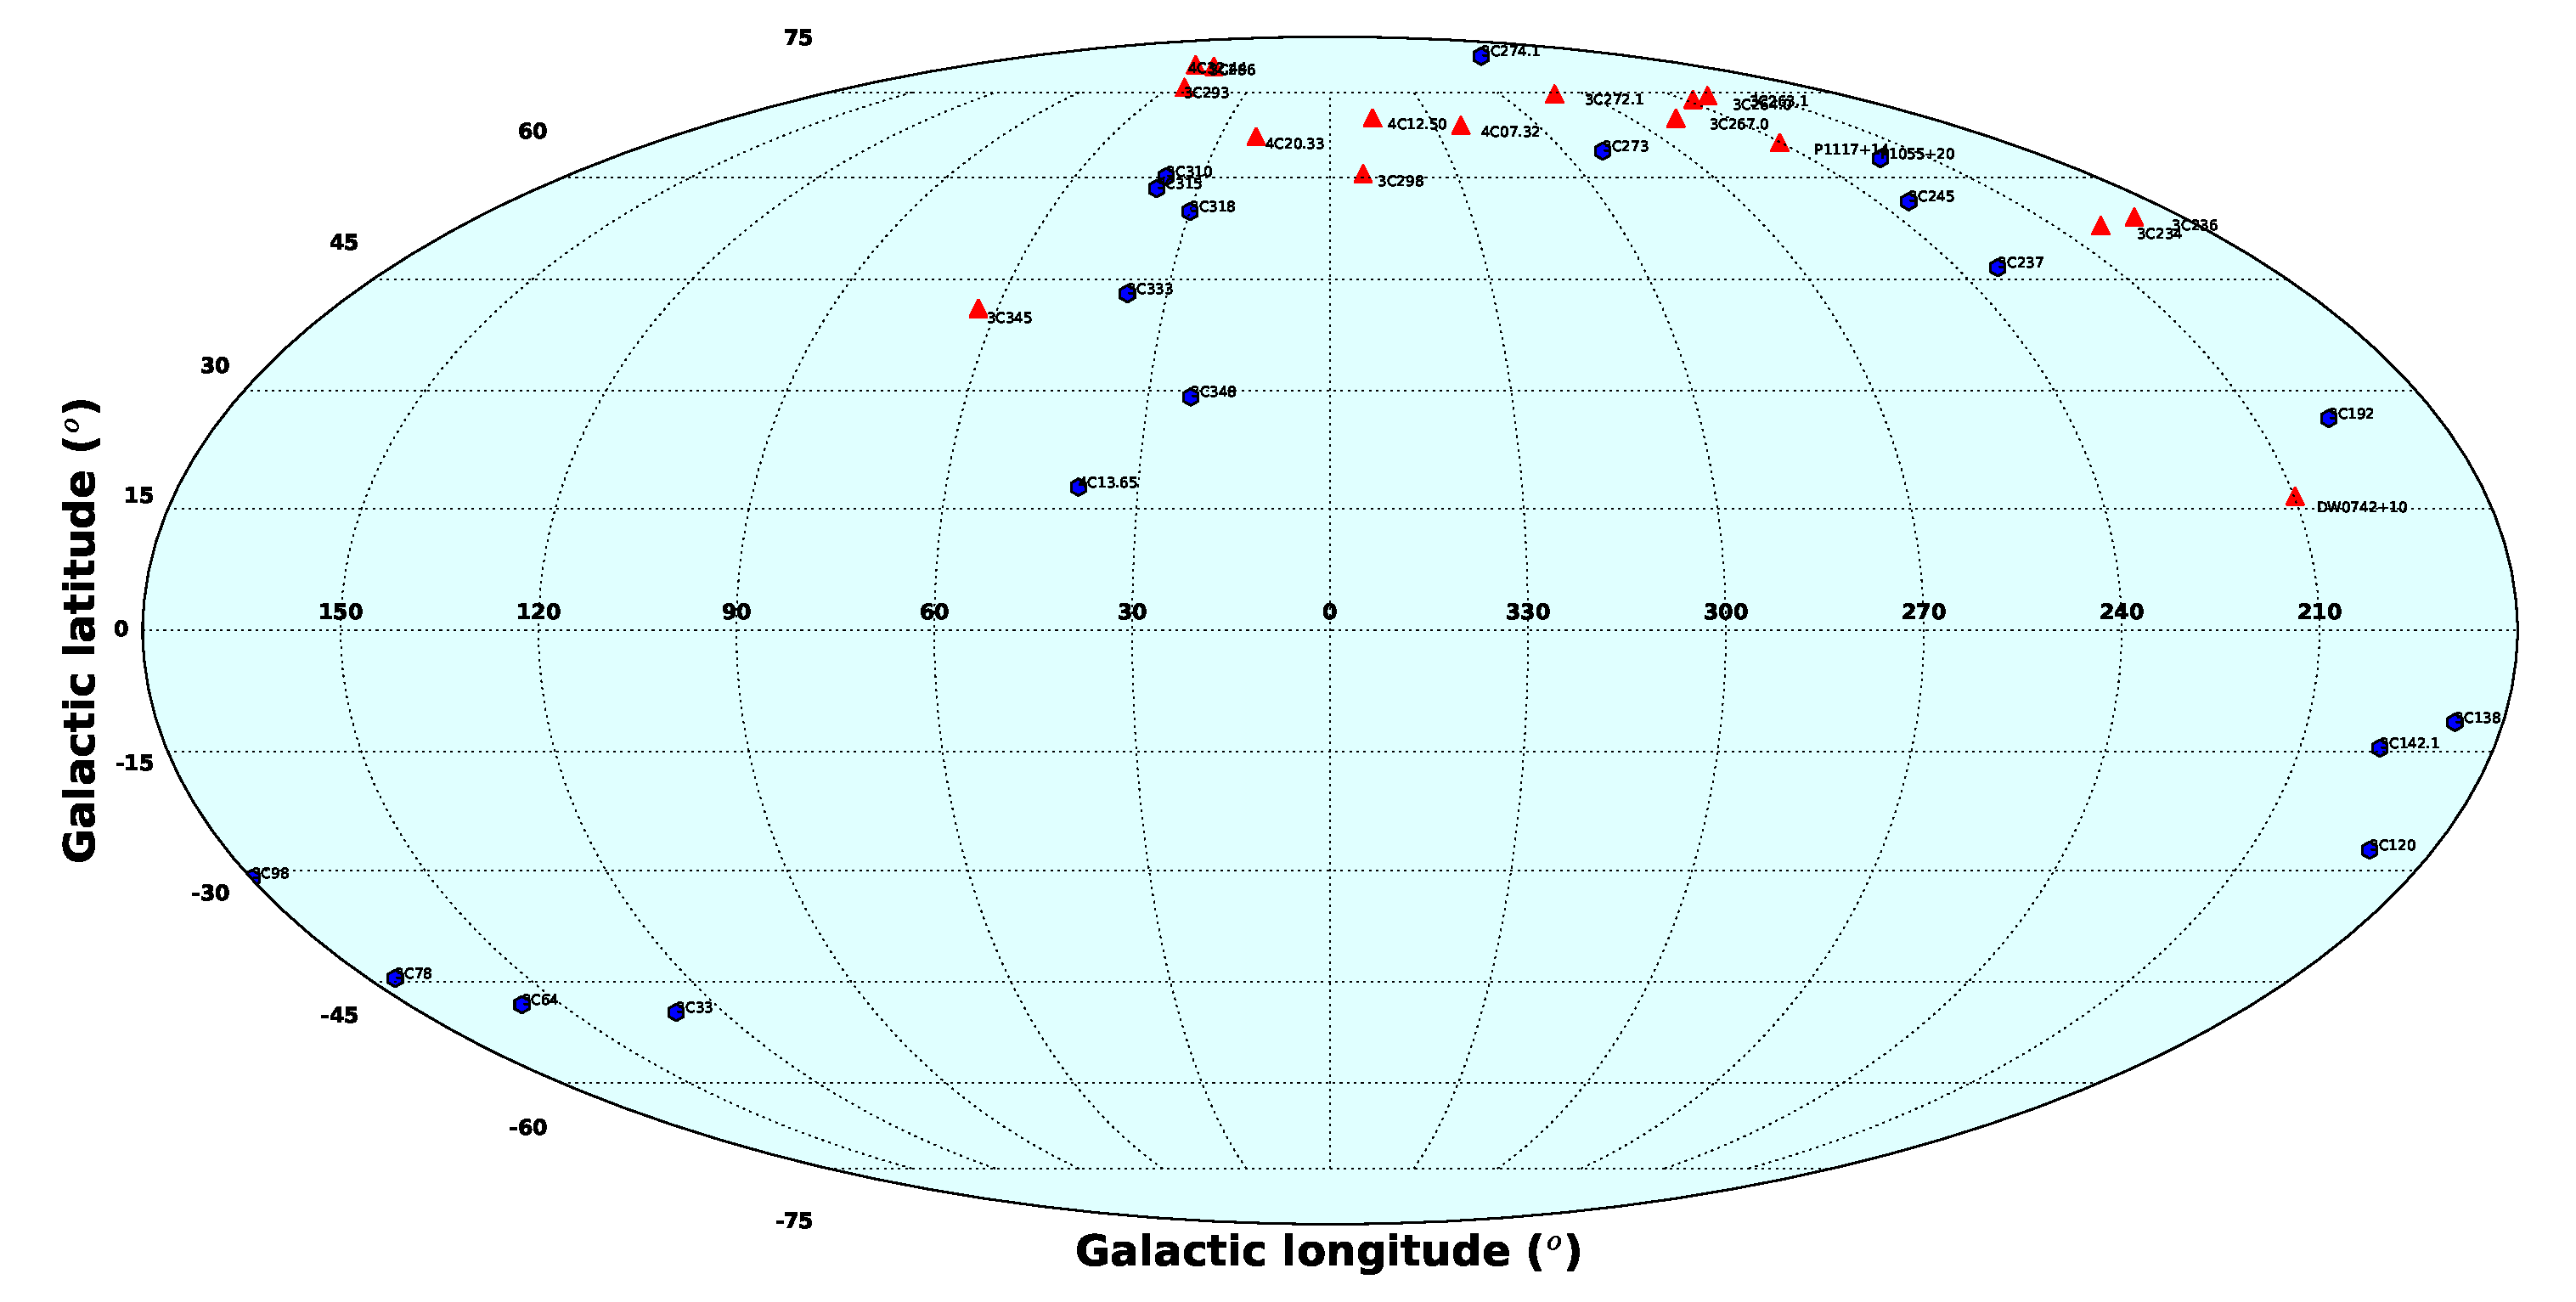
\includegraphics[width=\textwidth]{fig/src_locations.eps}
  \caption{Locations of all 93 sightlines considered in this study, overlaid on the map of dust optical depth \t353. Red symbols show the 35 sightlines designated as purely atomic; 19 observed in CO and OH with no detection (circles) and 16 low-\NHI\ (\NHI $<$3$\times$10$^{20}$cm$^{-2}$) sightlines (stars), assumed to be too diffuse for molecular gas. Black diamonds are sightlines observed in \hi\ only, which do not fall into the low-\NHI category. Blue triangles show molecular sightlines with at least one component detected in CO, and the purple triangle shows the single position detected in OH only (towards 3C132). The ``X'' marker labels the center of Milky Way.}
  \label{fig:src_locations}
\end{figure*}

We also show in Figure \ref{fig:ratio_vs_nhithin} the correlation between \NHI\ and \NHIthin\ towards all 93 positions. The ratio $f$=\NHI/\NHIthin\ increases linearly as a function log(\NHIthin/10$^{20}$) with a slope of (0.19$\pm$0.02) and an intercept of (0.89$\pm$0.02). This linear trend is consistent with those presented by \citet{Lee2015} (for the case of Persus molecular cloud), \citet{Heiles2003a} and \citet{Liszt2014}. 

% (slope: 0.32$\pm$0.06, offset: 0.81$\pm$0.05) for the case of Persus molecular cloud and HT03 (slope: 0.26$\pm$0.08, offset: 0.91$\pm$0.04 shown in Figure 13 in \citealt{Lee2015}). 
% These may suggest a general relation between \NHI\ and \NHIthin\ through out the Milky Way due to the large ranges for both Galactic latitude and longitude of the observed sightlines. If this is the case, optically thin \hi\ column density \NHIthin\ might be considered as the proxy for the total \hi\ column density \NHI. 

\begin{figure}
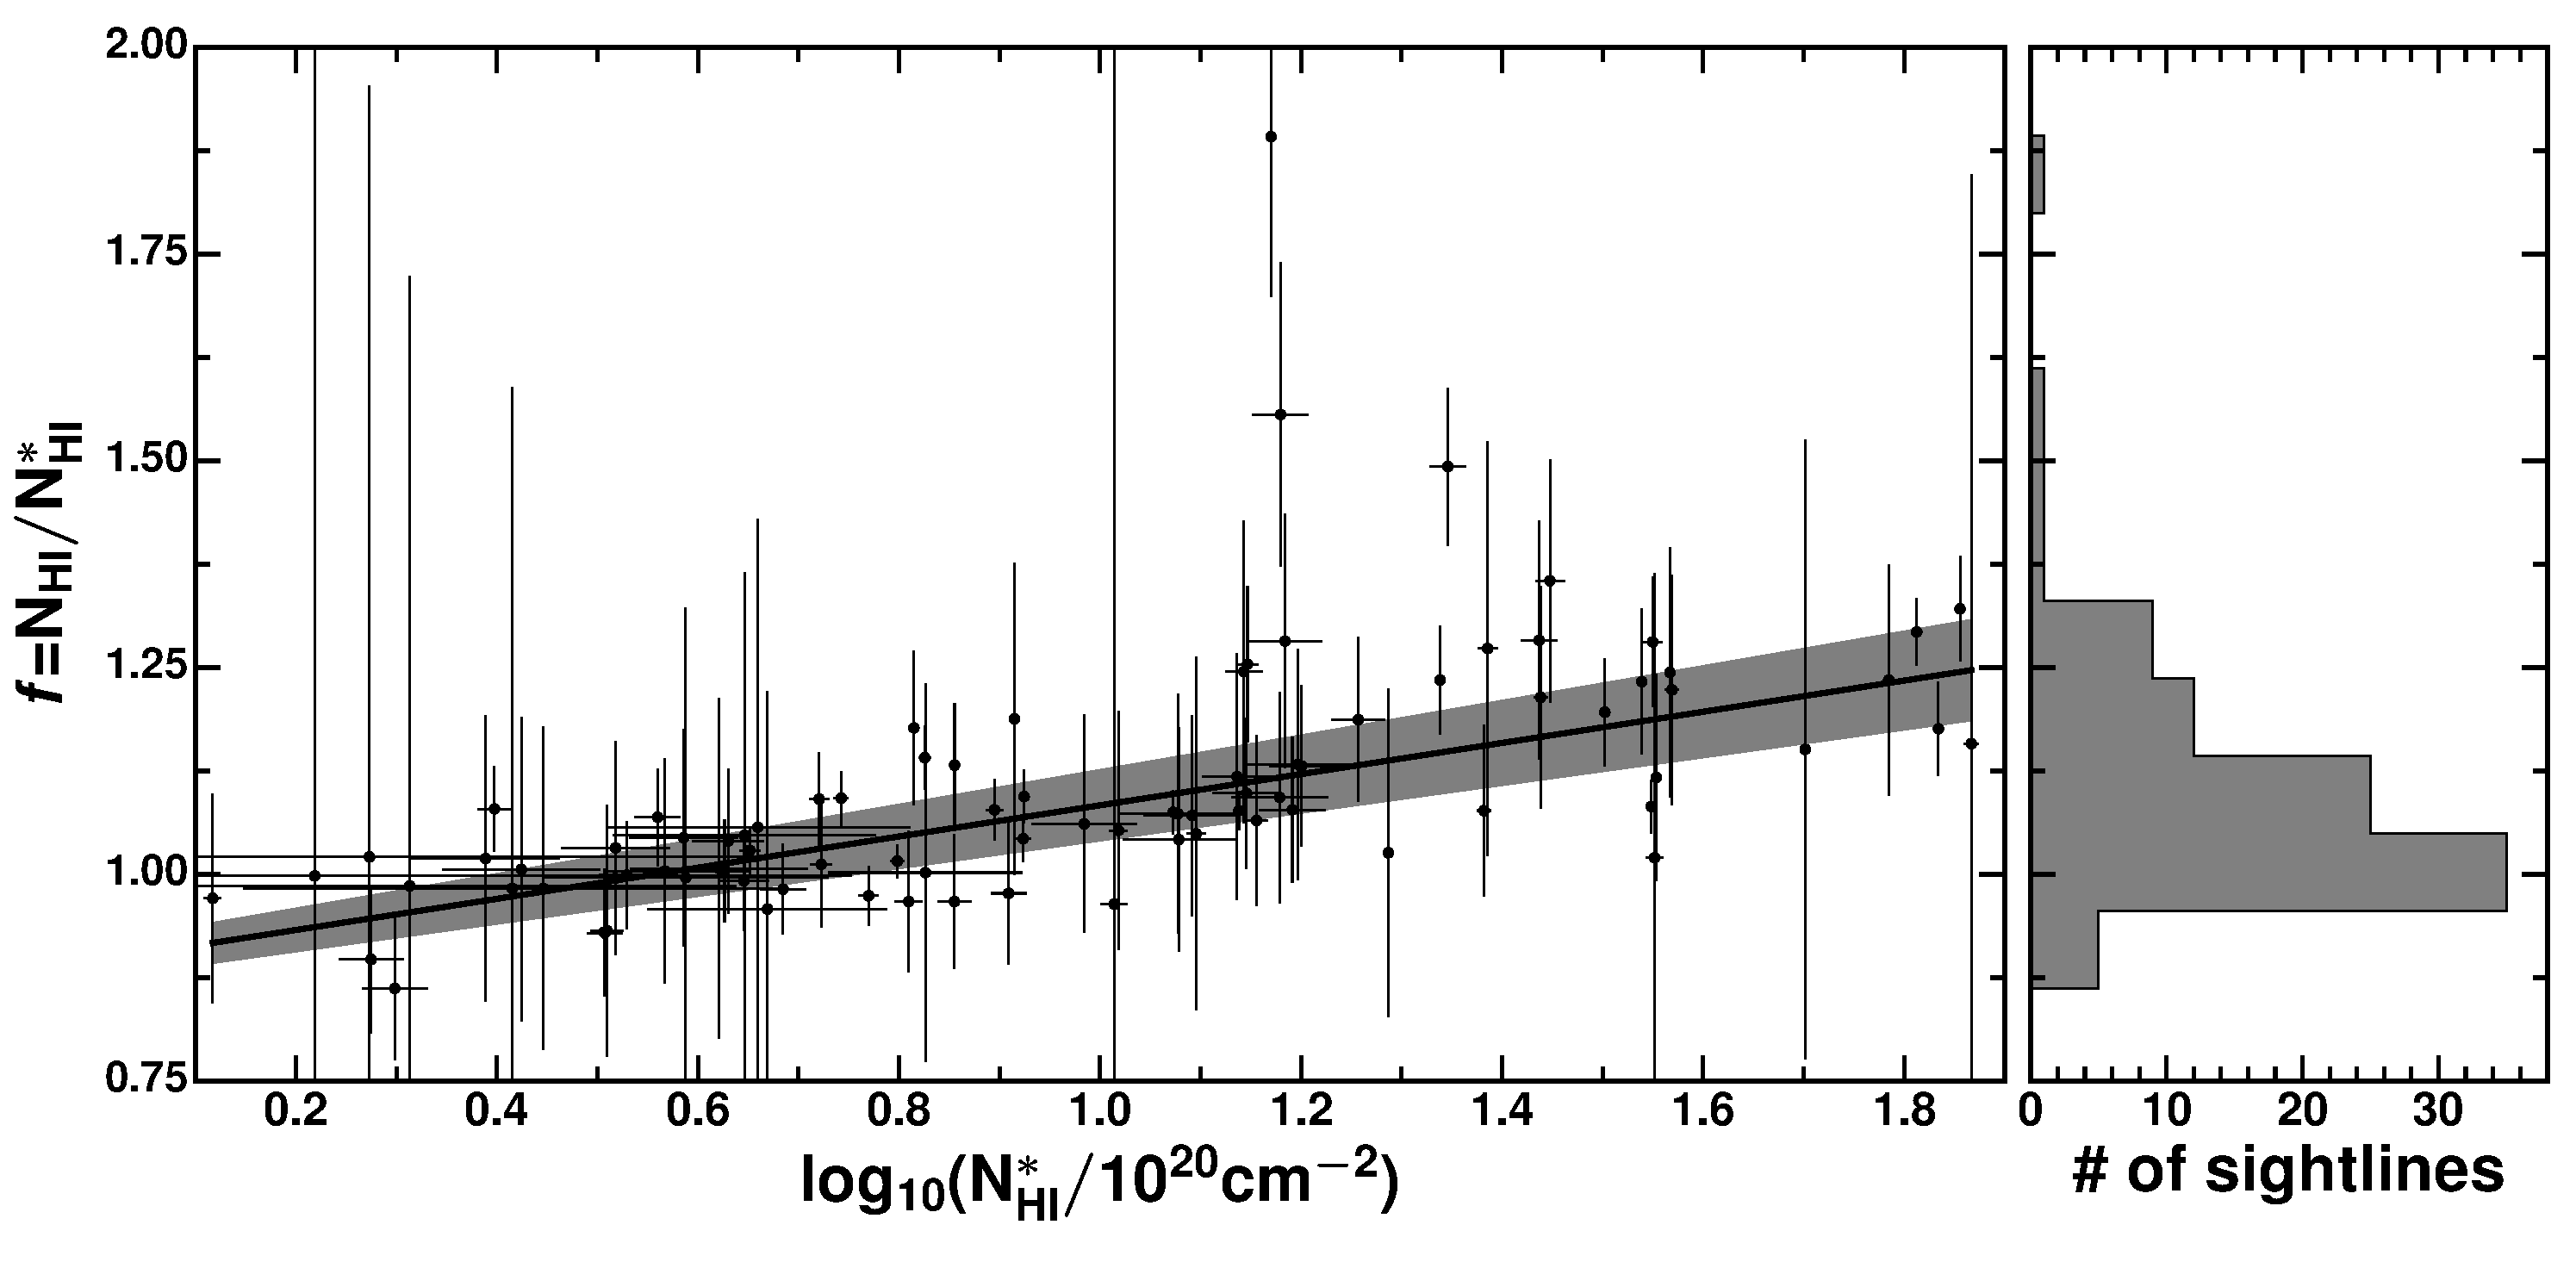
\includegraphics[width=1.0\linewidth]{fig/ratio_vs_nhithin.eps}
\caption{Left: The ratio $f$=\NHI/\NHIthin\ as a function of $log_{10}$(\NHIthin/10$^{20}$). The black solid line displays the linear fit to all 93 data points: $f$=$(0.19\pm0.02)log_{10}$(\NHIthin$/10^{20})$ + $(0.89\pm0.02)$. Right: Distribution of $f$=\NHI/\NHIthin.}
\label{fig:ratio_vs_nhithin}
\end{figure}

\subsection{CO}
\label{subsec:CO}
As described in \citet{Li2017}, a CO follow-up survey was conducted towards the 47 of the MS sightlines observed in OH. The J=1--0 transitions of \co, \13co, and \c18o\ were observed with the Delingha 13.7m telescope in China. \co(J=2--1) data for 45 sources and J=3--2 data for 8 sources with strong \co\ emission were taken with the 10.4m Caltech Submillimeter Observatory (CSO) on Mauna Kea. In this work we use CO data solely to identify and exclude from some parts of the analysis positions with detected CO-bright molecular gas -- {\color{blue} comprising 26 of the 48 observed positions}. These positions are identified in Figure \ref{fig:src_locations}. %The astronomical software package Gildas/CLASS\footnote{$http://www.iram.fr/IRAMFR/GILDAS/$} was used for reducing spectroscopic CO data obtained from single-dish telescopes. \par
%    \sout{[Due to the large uncertainty of X-factor converting CO integral intensity into \h2\ column density, we are ONLY interested in 26 sight-lines where CO emission lines are NOT detected. JO NOTE: Note to remind you to justify this decision in the context of the science we wish to do (which we will have laid out already in the intro probably.)]}
    
%\subsection{Planck/IRAS data for\\ thermal dust emission and color excess}
\subsection{Dust}
\label{subsec:data_planck_iras}
To trace the total gas column density \NH\ we use publicly-available all-sky maps of the 353 GHz dust optical depth (\t353) and radiance \rad\ from the Planck satellite. The \t353\ map was obtained by a modified black-body (MBB) fit to the first 15 months of 353, 545, and 857 GHz data, together with IRAS 100 micron data. For details, see PLC2014a. Both datasets have angular resolutions of 5 arcmin. In this work we use the R1.20 data release in Healpix\footnote{$http://healpix.sourceforge.net$} format (\citealt{Gorski2005}). %\sout{JO NOTE: I thought Marc-Antoine said not to use the Planck \ebv\ because it was essentially just a linear rescaling of another quantity (tau? R? I forget!)]}
As an alternative proxy for \NH, we also employ the all-sky \ebv\ map of \citet{Schlafly2011}, which used the spectral colors of stars in the Sloan Digital Sky Survey. 

%\section{Derivation of Optical Depth, Excitation Temperature and Column Density for OH(1665) and OH(1667)}
\section{OH Data Analysis}
\label{sec:derive_tex}

The Millennium Survey OH data consists of on-source and off-source ``expected'' spectra for every observed position in each of the OH lines (for further details see HT03). In our companion paper \citet{Li2017}, we use the method of HT03 to derive OH optical depths, excitation temperatures and column densities. Namely, we assume a two-phase medium and obtain solutions for $T_\mathrm{ex}$ and $\tau$ via Gaussian fitting (to both the on-source and off-source spectra) that explicitly includes the appropriate treatment of the radiative transfer. In the present work we use a simpler channel-by-channel method for the derivation of $T_\mathrm{ex}$, as described below. 

The radiative transfer equations for the on-source and off-source (expected) spectra %for ON/OFF source measurements 
may be written as:
\begin{equation}
T_\mathrm{B}^\mathrm{ON}(v) =(T_\mathrm{bg}+T_\mathrm{c})e^{-\tau_{v}} + T_\mathrm{ex}(1-e^{-\tau_{v}}) + T_\mathrm{rx}
\label{eq_ton}
\end{equation}
\begin{equation}
T_\mathrm{B}^\mathrm{OFF}(v)=T_\mathrm{bg}e^{-\tau_{v}} + T_\mathrm{ex}(1-e^{-\tau_{v}}) + T_\mathrm{rx}
\label{eq_toff} 
\end{equation}

\noindent Here $T_\mathrm{B}^\mathrm{OFF} (v)$ and $T_\mathrm{B}^\mathrm{ON} (v)$ are the main-beam temperatures of the off-source spectrum and on-source spectrum, respectively. $T_\mathrm{ex}$ is the excitation temperature, $\tau_{v}$ is the optical depth, $T_\mathrm{rx}$ is the receiver temperature ($\sim25$ K), and $T_\mathrm{c}$ is the main-beam temperature of the continuum source, which is assumed to be unresolved. %smaller than the main beam of the telescope. 
$T_\mathrm{bg}$ is the continuum background brightness temperature including the 2.7 K isotropic radiation from CMB and the Galactic synchrotron background at the source position. For consistency with HT03 and \citet{Li2017}, we estimate the synchrotron contribution at 1665.402 MHz and 1667.359 MHz from the 408 MHz continuum map of \citet{Haslam1982}, by adopting a temperature spectral index of 2.8, such that
\begin{equation}
T_\mathrm{bg} = 2.7 + T_\mathrm{bg,408}(\nu_\mathrm{OH}/408)^{2.8},
\label{eq4c} 
\end{equation}
\noindent resulting in typical values of around 3.5 K. The  background continuum contribution from Galactic HII regions may be safely ignored, since the continuum sources we observed are either at high Galactic latitudes or Galactic Anti-Center longitudes. %We assume $T_\mathrm{rx}\sim 25$ K. % in Stokes I parameter (or $\sim25$ K in brightness temperature). 
Thus, in line-free portions of the off-source spectra:
\begin{equation}
T_\mathrm{B}^{OFF}(v)= T_\mathrm{bg} + T_\mathrm{rx}.
\label{eq_toff_offline}
\end{equation}
In the absence of information about the true gas distribution, we assume that OH clouds cover fully both the continuum source and the main beam of the telescope. %The beam efficiency is of Arecibo telescope at 1666MHz is $\sim0.48$, \sout{which is a reasonable assumption for Arecibo} for which $\sim90\%$ of the power is contained within the main beam and inner sidelobe. Therefore, we can assume that the antenna temperature equals the brightness temperature of the OH lines ????.
%In this work we use a simple method solving the two Transfer 
We may therefore solve equations (\ref{eq_ton}) and (\ref{eq_toff}) to derive $T_\mathrm{ex}$ and $\tau_{v}$ for each of the OH lines on a channel-by-channel basis:
\begin{equation}
e^{-\tau_{v}} = \frac{T_\mathrm{B}^\mathrm{ON}(v) - T_\mathrm{B}^\mathrm{OFF}(v)}{T_\mathrm{c}},
\label{eq_etau} 
\end{equation}
\begin{equation}
T_\mathrm{ex} = \frac{T_\mathrm{B}^\mathrm{OFF}(v)-T_\mathrm{bg}e^{-\tau_{v}} - T_\mathrm{rx}}{1-e^{-\tau_{v}}}.
\label{eq_tex}
\end{equation}
\noindent %The procedure is described as follows: \par
%1. Compute the opacity spectrum $e^{-\tau_{v}}$ (as well as optical depth spectrum $\tau_{v}$ and its RMS $\sigma_{\tau_{v}}$) by using equation \ref{eq_etau}. \par
We fit each OH opacity spectrum (given by Equation \ref{eq_etau}) with a set of Gaussian profiles %to estimate the physical properties of OH clouds along the line-of-sight, each component is assumed to correspond to a single OH clump: \sout{[JO NOTE: reword to make it clear that Gaussian fits only used to later identify positions of lines.tx]}
%\begin{equation}
%\tau(v) = \sum\limits_{n=0}^{N-1} \tau_{0,n}e^{-[(v-v_{0,n})/\delta v_{n}]^2}. 
%\label{tau_ngauss} 
%\end{equation}
%\noindent This least-squares fit gives 
to obtain the peak optical depth ($\tau_{0,n}$), central velocity ($v_{0,n}$) and FWHM ($\Delta v_{n}$) of each component, $n$. %These fits are used only to identify the positions and the widths of the lines. 
Equation (\ref{eq_tex}) is then used to calculate excitation temperature spectra. Examples of $e^{-\tau_{v}}$, $T_\mathrm{B}^\mathrm{OFF}$, and $T_\mathrm{ex}$ spectra are shown in Figure \ref{fig:example_p042820}, together with their associated Gaussian fits. It can be seen that the $T_\mathrm{ex}$ spectra are approximately flat within the FWHM of each Gaussian component. %Hence, we choose only the range within the width $\delta v_{n}$ from $(v_{0,n}-\delta v_{n}/2)$ to $(v_{0,n}-\delta v_{n}/2)$ to 
We therefore compute an excitation temperature for each component from the mean $T_\mathrm{ex}$ in the range $v_{0,n} \pm \Delta v/2$. %For the case of 3C123, we adopted the value of T$_{bg}$ to be 25.0 K (reason why??).

Figure \ref{fig:tex_tau_compare} compares the peak $\tau$ and \Tex\ values obtained from our method with those of \citet{Li2017}, demonstrating that the two methods return very consistent results. % using the Gaussian decomposition method. We agree with their conclusions namely the optical depths for the OH main lines satisfy the optically-thin assumption and, in general, the two main lines are not in LTE. 
Minor differences arise only for the most complex sightlines through the Galactic Plane (G197.0+1.1, T0629+10) where the spectra are not simple to analyze; however, even these points are mostly consistent to within the errors. 
 %, and discussed further below. The comparisons of $\tau$ and \Tex\ obtained from the 2 methods are shown in Figure \ref{fig:tex_tau_compare}. 

\par
We compute total OH column densities, $N_\mathrm{OH}$, independently from both the 1667 and 1665 MHz lines via: %components independently using the following equations:
%\begin{equation}
%N_{\mathrm{OH}(1667)}=\frac{8\pi kT_{ex,1667}{{\nu}^2_{1667}}}{A_{1667}c^{3}h}\frac{16}{5}\int\tau_{1667}dv\ (cm^{-2})
%\label{eq_noh67}
%\end{equation}
%\begin{equation}
%N_{\mathrm{OH}(1665)}=\frac{8\pi kT_{ex,1665}{{\nu}^2_{1665}}}{A_{1665}c^{3}h}\frac{16}{3}\int\tau_{1665}dv \ (cm^{-2})
%\label{eq_noh65}
%\end{equation}

\begin{equation}
\frac{N_{\mathrm{OH,1667}}}{[10^{14}~\mathrm{cm}^{-2}]}=2.39 \cdot \tau_{1667} \cdot \frac{T_\mathrm{ex,1667}}{[K]} \cdot \frac{\Delta v_{1667}}{[\mathrm{km~s}^{-2}]},
\label{eq_noh67rd}
\end{equation}
\begin{equation}
\frac{N_{\mathrm{OH,1665}}}{[10^{14}~\mathrm{cm}^{-2}]}=4.30 \cdot \tau_{1665} \cdot \frac{T_{\mathrm{ex},1665}}{[K]} \cdot \frac{\Delta v_{1665}}{[\mathrm{km~s}^{-2}]},
\label{eq_noh65rd}
\end{equation}

\noindent where the constants include Einstein A-coefficients of $A_{1667}=7.778\times 10^{-11} s^{-1}$ and $A_{1665}=7.177\times 10^{-11} s^{-1}$ for the OH main lines (\citealt{Destombes1977}). All values of $\tau$, $T_\mathrm{ex}$ and $N_\mathrm{OH}$ are tabulated in Table \ref{table:OH-parameters}. %Substituting the constants into the above equations, they can be written as:

\begin{figure}
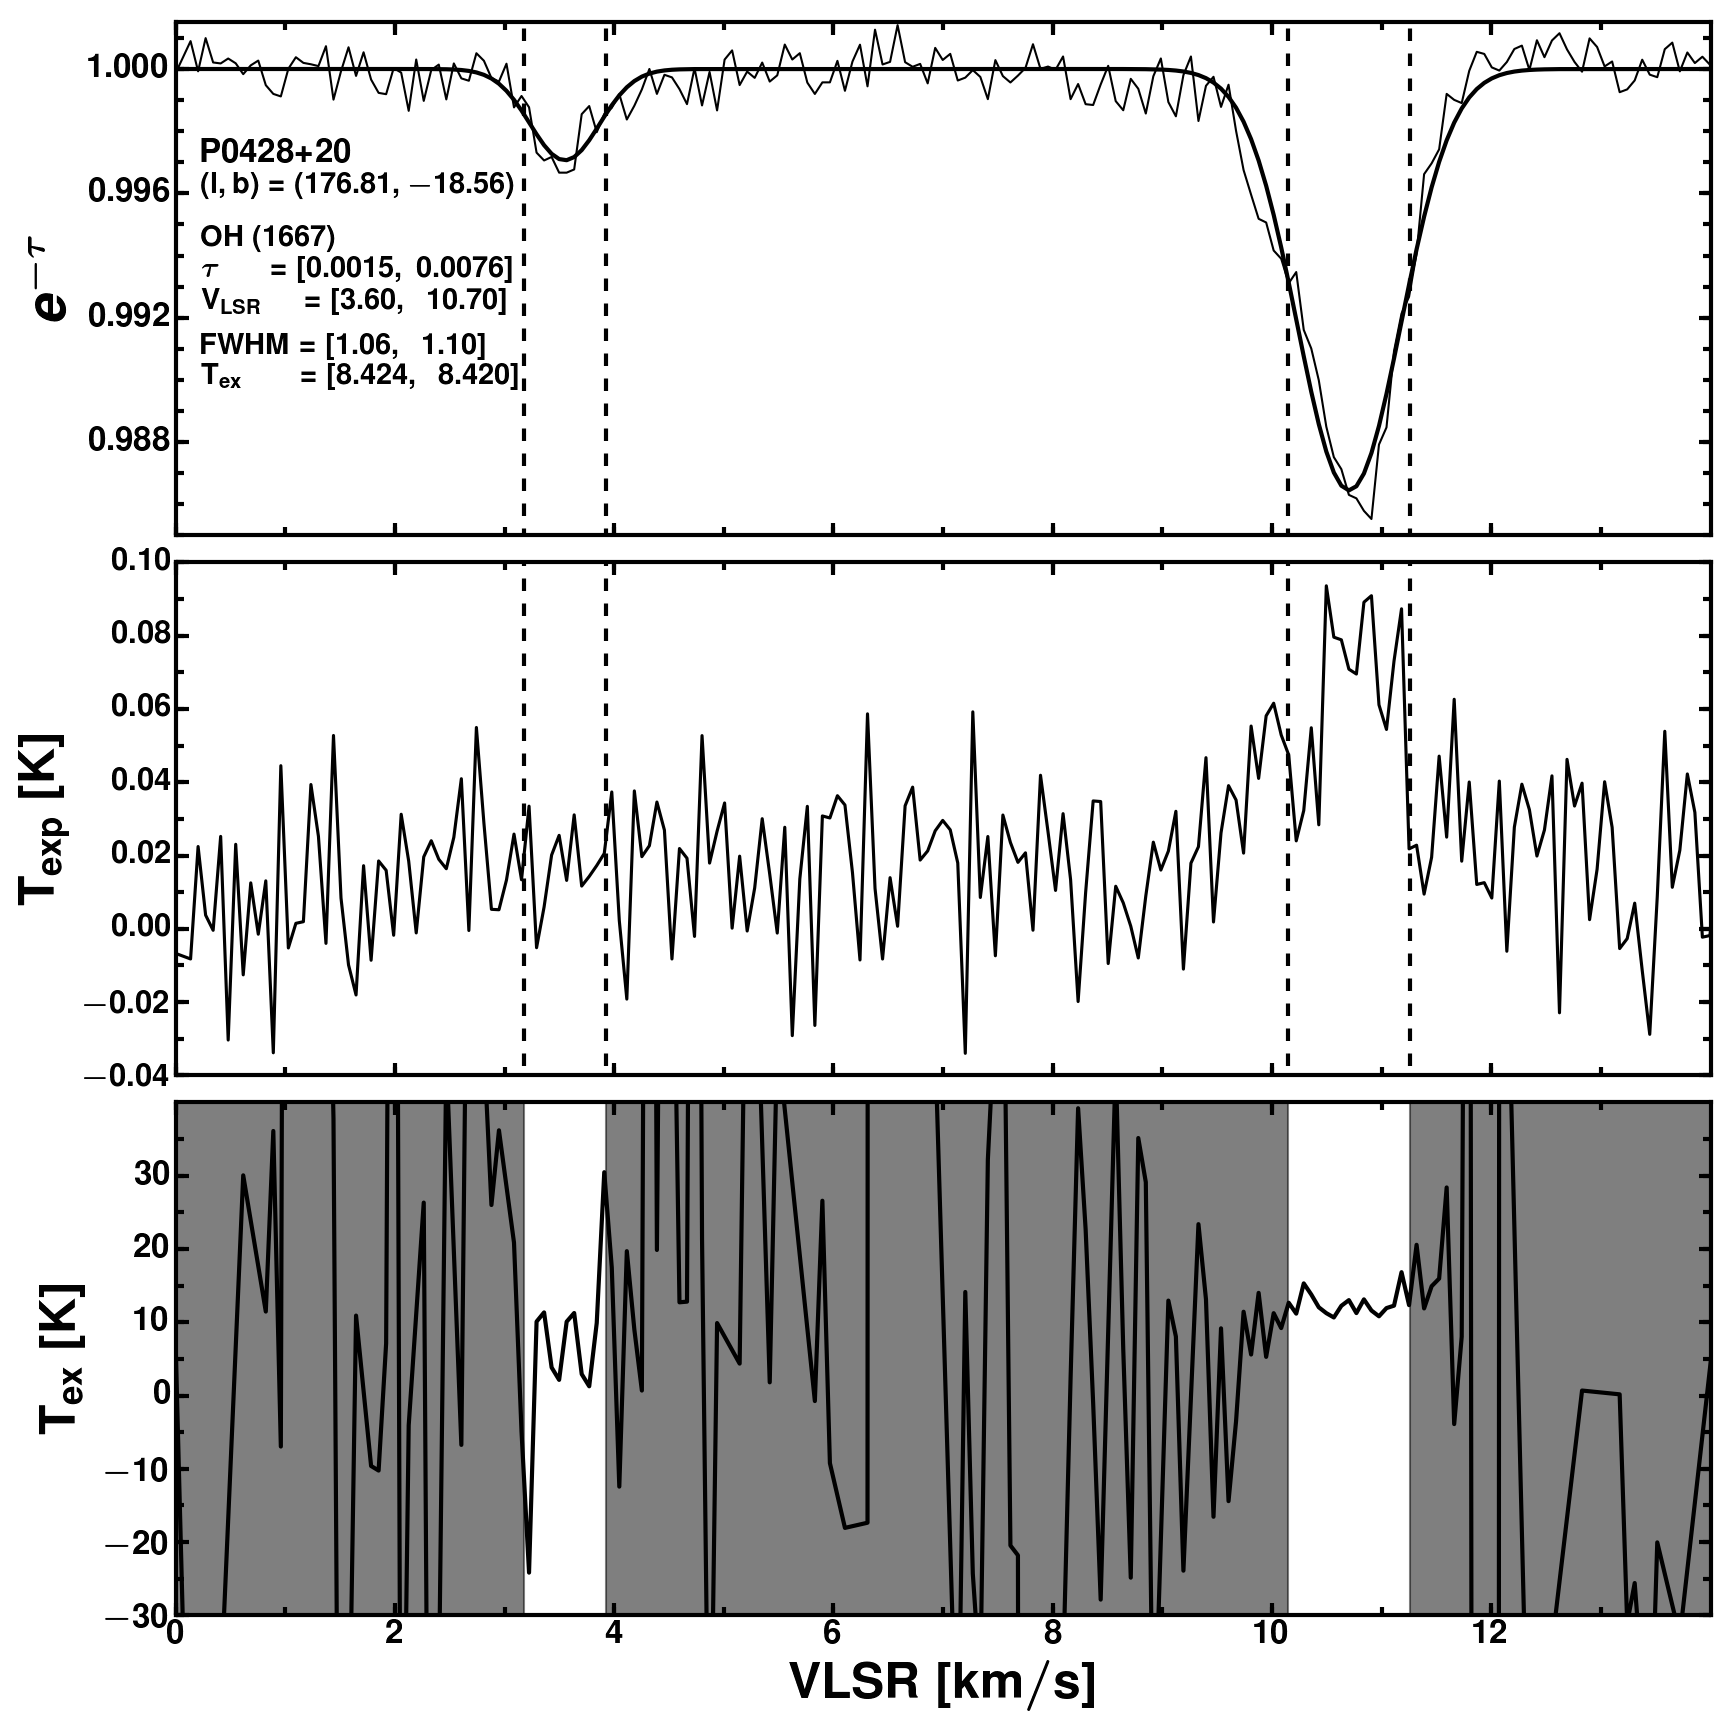
\includegraphics[width=1.0\linewidth]{fig/tex_spec_P0428+20.eps}
\caption{Example of OH 1667 MHz $e^{-\tau_{v}}$ (top), expected $T_\mathrm{B}^\mathrm{OFF}$ (middle), and $T_\mathrm{ex}$ (bottom) spectra for the source P0428+20. The FWHM of the Gaussian fits to the absorption profile are used to define the range over which $T_\mathrm{ex}$ is computed for each component, shown as white regions in the bottom panel.}
%Illustration of derived parameters from the fit to the absorption profile (upper panel), the expected emission (middle panel) profile and \Tex\ spectrum (lower panel) for the source P0428+20. The vertical dashed-lines display the FWHM of Gaussian components.}
\label{fig:example_p042820}
\end{figure}



\begin{figure}
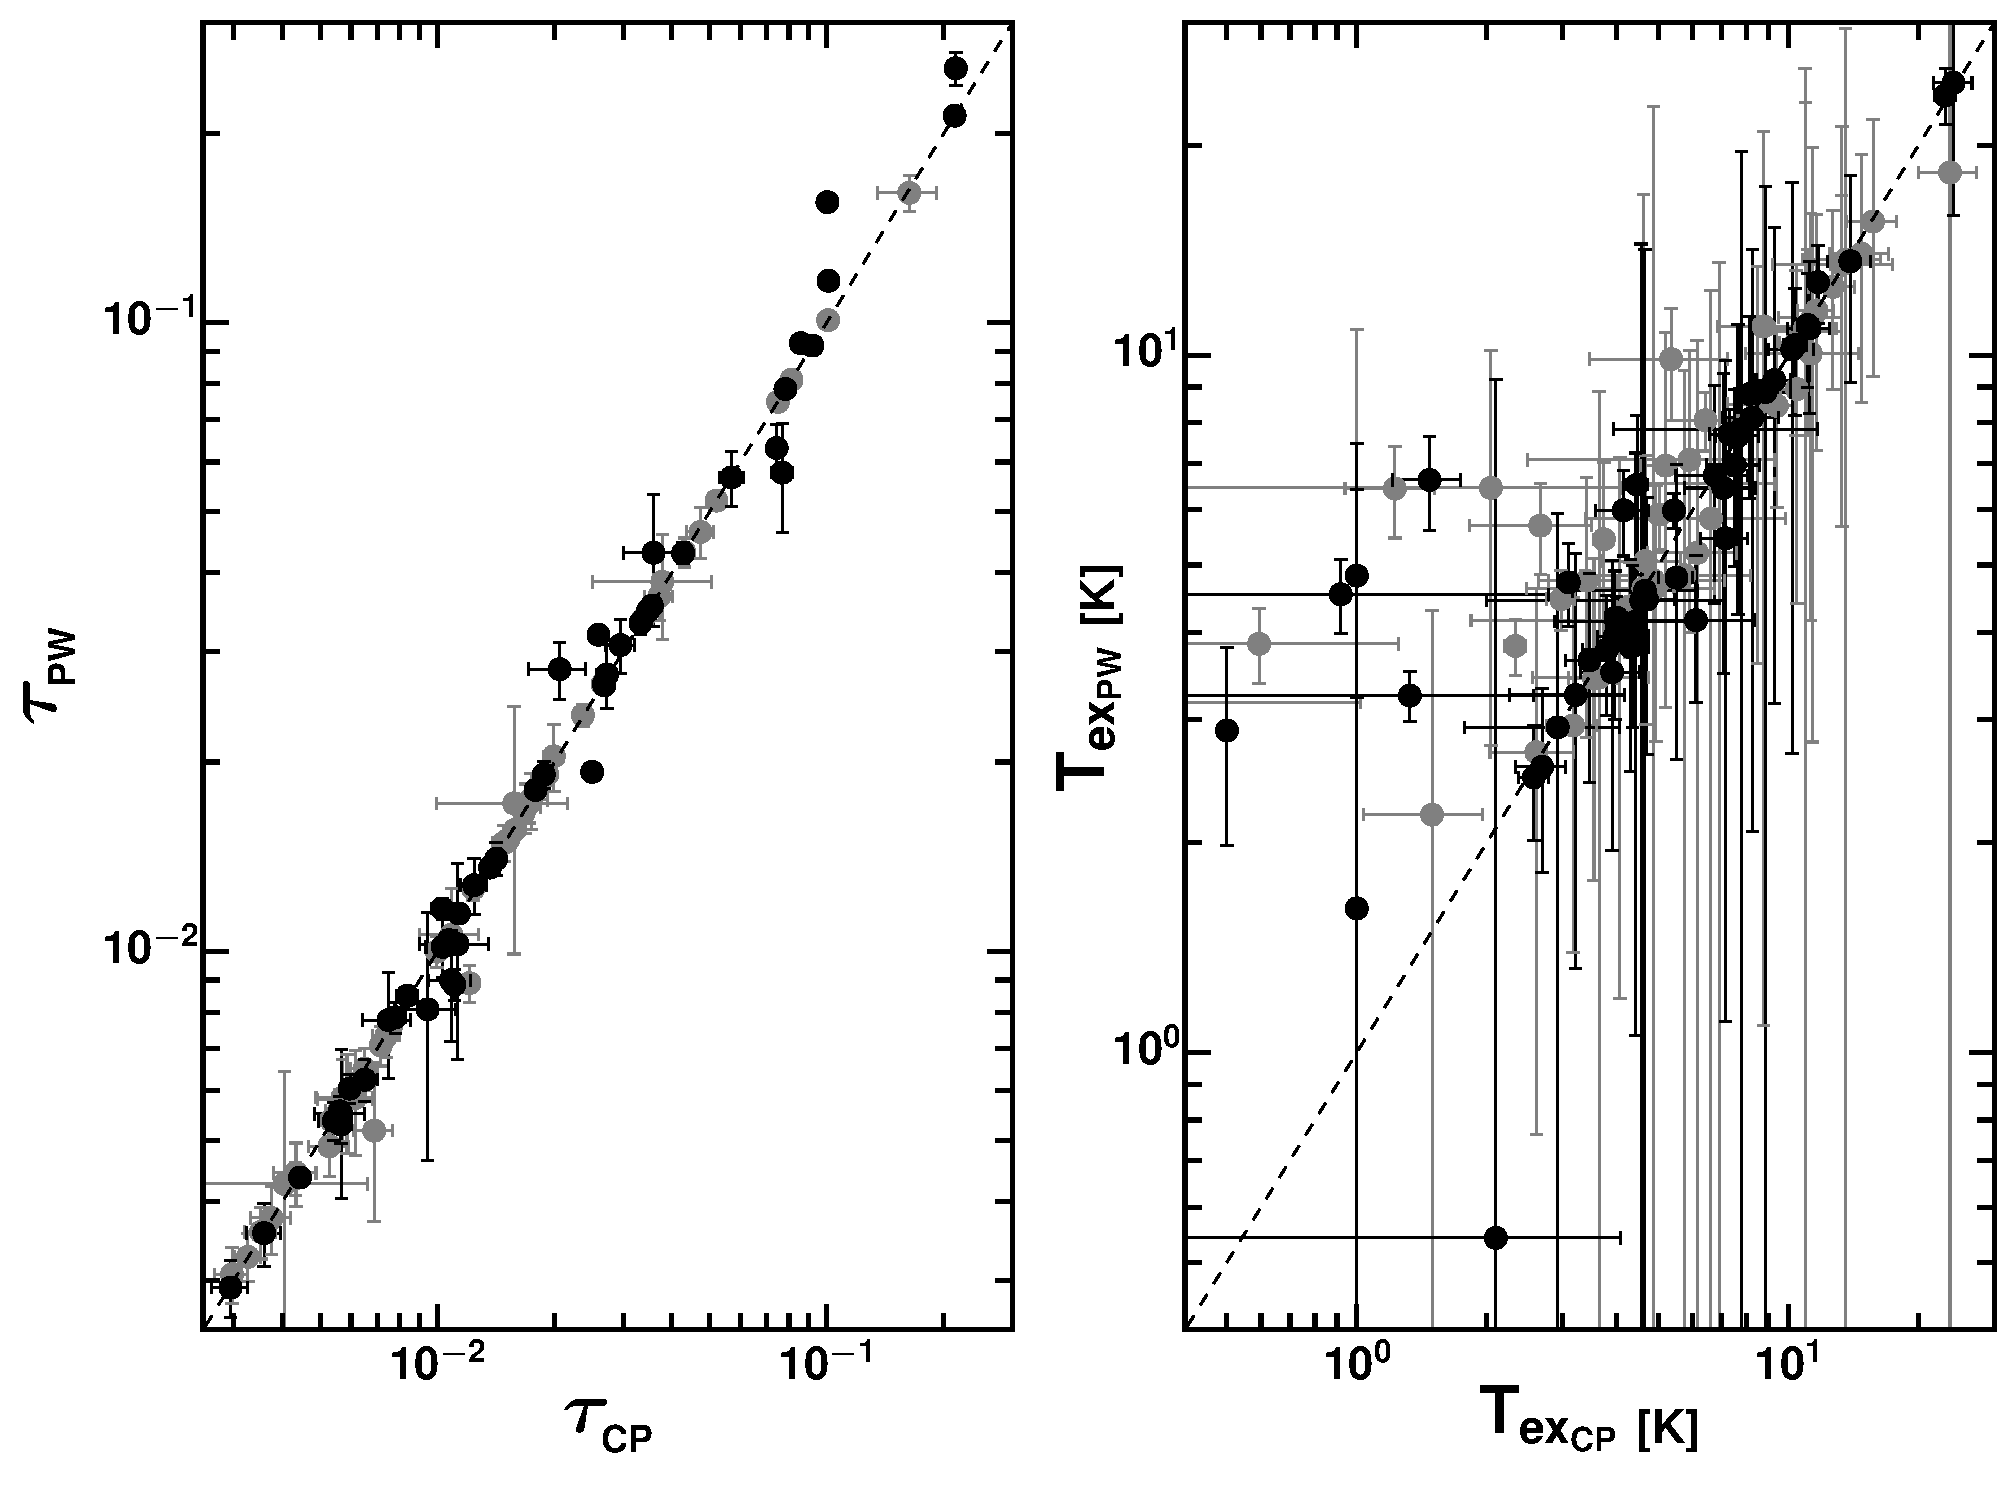
\includegraphics[width=1.0\linewidth]{fig/tex_tau_compare.eps}
\caption{Comparison between derived values of the peak optical depth $\tau_0$ (left panel), and \Tex\ (right panel) for both OH mainlines, 1667 MHz (black) and 1665 MHz (gray), as obtained from our companion paper by \citet{Li2017} (subscript CP) and the present work (subscript PW). The dashed lines mark where the two values are equal.}
\label{fig:tex_tau_compare}
\end{figure}

\begin{figure*}
 \center
  \includegraphics[width=\textwidth]{fig/src_examples.eps}
  \caption{Examples of 4 sighlines towards radio sources in 4 different dust maps (3$\times$3 degrees in Galactic coordinates) adopted from Planck collaboration 2014 ($\tau_{353}$, radiance and dust temperature, Nside = 1024) and \citealt{Schlafly2011} (\ebv, Nside = 512). The `X' markers at centers show the locations of the sources. The contours represent the integrated intensity W$_{CO(1-0)}$ from \citealt{Dame2001}.}
  \label{fig:src_examples}
\end{figure*}

\section{Dust-Based Proxies for Total neutral gas\\ column density}
\label{sec:proxies-for-nh}
In this section we will investigate the correlations between dust properties and the total gas column density \NH. Specifically, we consider dust optical depth at 353 GHz, \t353, dust radiance, \rad, reddening, \ebv, with datasets sourced as described in Section \ref{subsec:data_planck_iras}. When these quantities are used as proxies for \NH, the underlying assumption is that a single linear relationship holds between the measured quantity and \NH. In this work, our sample of \hi\ emission/absorption pairs provides accurate (opacity-corrected) \hi\ column densities, while complementary OH and CO data allow us to identify, and optionally exclude, sightlines with molecular gas (dark or not). 

In the following, we consider the subsample of 34 purely atomic sightlines, where either CO and OH are observed and not detected (16 sightlines), or where CO is not observed and OH is not detected (18 sightlines). Here we set the detection limit for OH 1667MHz line at 10$^{13}$cm$^{-2}$ according to \citet{Li2017}.
Thus, we are confident to assume that there is only neutral hydrogen along these 34 sightlines, most of them (33 sightlines) are outside the Galactic plane $|$b$|$$>$10$^{o}$. Figure \ref{fig:src_examples} shows the examples of 4 sightlines in the maps of \t353, \ebv, dust radiance and dust temperature. %\sout{[JO NOTE: Stress this is an excellent assumption]}.

We are therefore able to compare the performance of the various proxies along a sample of purely atomic sightlines within a moderate \NHI\ range, which includes dust optical depth \t353, dust radiance \rad, dust reddening \ebv\ and investigate the origin of the departures from linearity seen by PLC2014a in the low-to-moderate range (1$-$122)$\times10^{20}$cm$^{-2}$.

In all following subsections, \NH\ is therefore assumed to be equal to \NHI, the opacity-corrected H{\sc i} column density, derived along sightlines with no molecular gas.

\subsection{ \NH\ from dust optical depth \t353}
\label{subsec:nh-from-t353}
We adopt the all-sky map of dust optical depth \t353 computed by PLC2014a. This was derived from a modified black body (MBB) empirical fit to IRAS and Planck maps at 3000, 857, 545 and 353 GHz, described by the expression %\sout{\color{red}[JO (16/6/17): make it clear that its not us who did this work]}:

\begin{equation}
I_{\nu} = \tau_{353}B_{\nu}(T_\mathrm{obs})\left(\frac{\nu}{353}\right)^{\beta_\mathrm{obs}}
\label{eq_mbbfit}
\end{equation}

\noindent Here, optical depth \t353, dust temperature $T_\mathrm{obs}$ and spectral index $\beta_\mathrm{obs}$ are the three free parameters, and $B_{\nu}(T_\mathrm{obs})$ is the Planck function for dust at temperature $T_\mathrm{obs}$ which is, in this model, considered to be uniform along each sightline (see PLC2014a for more details).
%In the optically thin limit (an accurate assumption), t
The relation between dust optical depth \t353 and total gas column density \NH\ can then be written as:

\begin{equation}
\tau_{353} = \frac{I_{353}}{B_{353}(T_\mathrm{obs})} = \kappa_{0}r\mu m_{H}N_{H} = \sigma_{353}N_{H}
\label{eq_t353_nh}
\end{equation}

\noindent where \s353\ is the dust opacity, $\kappa_{0}$ is the dust emissivity cross-section per unit mass (cm$^{2}$ g$^{-1}$), $r$ is the dust-to-gas mass ratio, $\mu$ is the mean molecular weight and $m_{H}$ is the mass of a hydrogen atom.

Figure \ref{fig:tau_vs_nhi} shows the correlation between  \NH\ and \t353. A tight linear trend can be seen with a Pearson coefficient of 0.95. The value of \s353\ from the ODR linear fit is $(7.2\pm 0.3){\times}10^{-27}$ cm$^{2}$ H$^{-1}$, consistent with that obtained by PLC2014a, $(6.6\pm 1.7){\times}10^{-27}$ cm$^{2}$ H$^{-1}$. Note that here we have quoted the PLC2014a measurement made towards low \NHI\ positions, since the lack of any \hi\ opacity correction in that work makes this value the most reliable. However, our fit is consistent with all of \s353\ values presented in that work, to within the quoted uncertainties. %\sout{[[JO NOTE: Will need some explanation on the two values from the Planck paper, what they mean, and why the black one is thought to be the best one. Can/should we consider fitting just the low column density points (as Marc-Antoine did to get the black line) and seeing what we get?]]}. 

\begin{figure}[h]
\centering
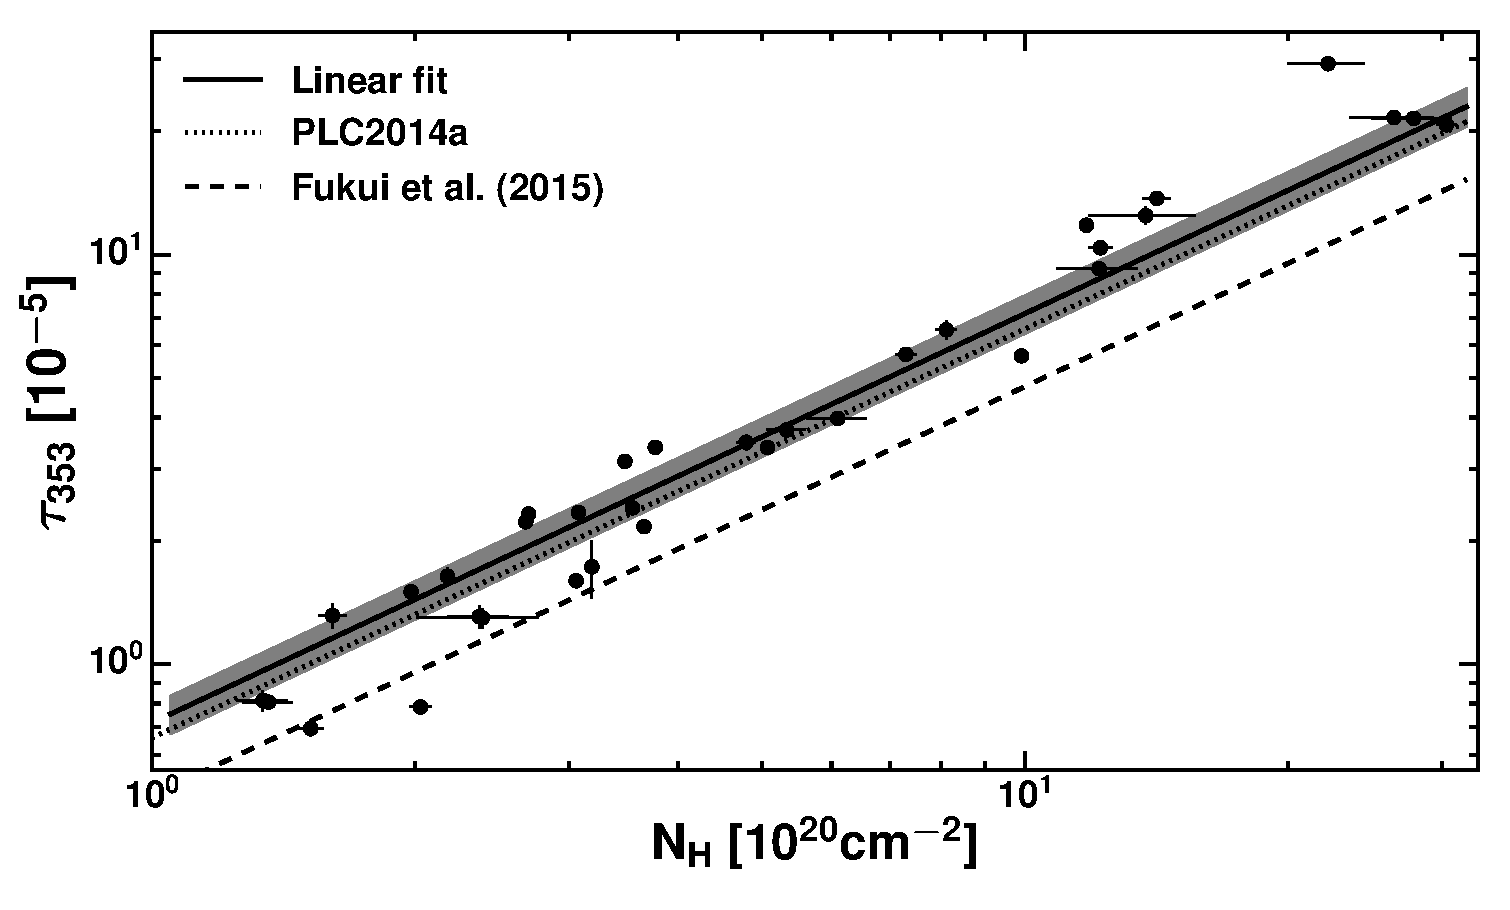
\includegraphics[width=1.0\linewidth]{fig/tau_vs_nh.eps}
\caption{\t353\ vs \NH\ along the 34 purely atomic sightlines described in the text. The thick solid line shows the linear fit to the data, the dotted-line shows the conversion factor from PLC2014a, and the dash line shows the conversion factor derived by \citet{Fukui2015}.}
\label{fig:tau_vs_nhi}
\end{figure}

A systematic deviation of data points above the fit line is seen at higher column densities, indicating an excess of \t353\ over the linear relation with \NH. Since we have accounted for all gas along these sightlines, the implication is that such deviations cannot be explained by the presence of unaccounted Dark Gas, and must instead have an alternative origin. We will discuss this further below.

The dust opacity \s353\ derived by \citet{Fukui2015} is plotted as a dash line. These authors derived a smaller value than in the present work (by a factor of $\sim$0.7), by restricting their fit to only the warmest dust temperatures, under the assumption that these most reliably select for genuinely optically thin \hi. %under the assumption that optically thick \hi can be recovered based on dust temperatures (??? or something ???). 
They then %applied their value on large-scales, and 
combined their derived values of \NH\ with a simple single-component model for the atomic medium, to suggest that significantly more optically thick \hi\ (CNM) exists than is usually assumed. However, their \s353\ is significantly different to the value we derive here based on ``true'', opacity-corrected \hi\ column densities, and by extension, applying it to \t353 at our source positions significantly overestimates \NHI. Our results therefore appear inconsistent with their picture that the dark ISM in the Milky Way is dominated by the optically thick \hi.

\subsection{ \NH\ from dust radiance \rad}
\label{subsec:nh-from-radiance}
Dust radiance (also known as dust integrated intensity) is may be defined as:

\begin{equation}
\begin{split}
\mathcal{R} = \int_{\nu}^{} I_{\nu}~d\nu = \int_{\nu}^{} \tau_{353}B_{\nu}(T_\mathrm{obs})\left(\frac{\nu}{353}\right)^{\beta_\mathrm{obs}}~d\nu\\
= G_{0}\sigma_{a}r\mu m_{H} N_{H}
\end{split}
\label{eq_r_nh}
\end{equation}
\noindent where $G_{0}$ is the intensity of the ambient radiation field, $\sigma_{a}$ is the grain absorption cross-section. These two quantities do not vary significantly in the diffuse ISM at high Galactic latitude.

\begin{figure}
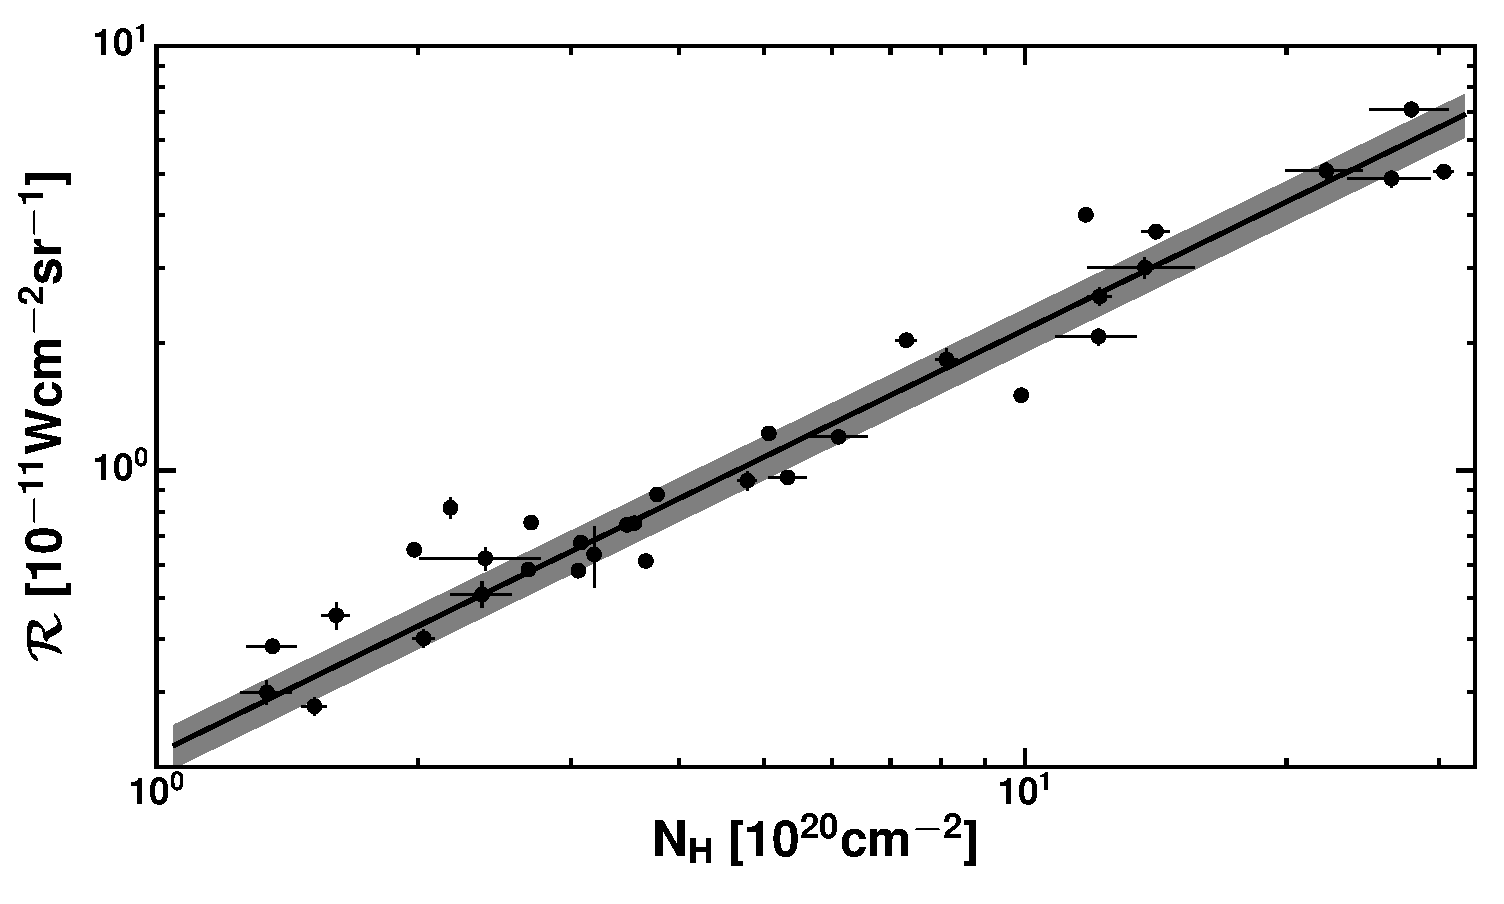
\includegraphics[width=1.0\linewidth]{fig/r_vs_nh.eps}
\caption{Dust radiance \rad\ as the function of total gas column density \NH\ along 34 atomic sightlines.}
\label{fig:r_vs_nh}
\end{figure}

Figure \ref{fig:r_vs_nh} plots \rad\ as a function of \NH. An ODR linear fit was performed, resulting in a slope of \NH/\rad=(4.65$\pm$0.17)$\times$10$^{31}$$W^{-1}sr$. {\color{magenta} This is 1.24 times higher than} the value of (3.75$\pm$0.08)$\times$10$^{31}$$W^{-1}sr$ obtained by PLC2014a. The Pearson coefficient is 0.96 -- slightly higher than for \t353. 

\subsection{ \NH\ from dust reddening \ebv}
\label{subsec:nh-from-ebv}
Reddening caused by the absorption and scattering of light by dust % and other matter in the interstellar medium 
is defined as:

\begin{equation}
\begin{split}
E(B{-}V) = \frac{A_{V}}{R_{V}} = \frac{ \sigma_{a} }{ R_{V} } r \mu  m_{H} N_{H}
\end{split}
\end{equation}

\noindent where \av\ is the dust extinction, $R_V$ is an empirical coefficient correlated with the average grain size, %of the dust grains causing the extinction, 
and all other symbols are defined as before. In the Milky Way, $R_{V}$ is typically {\color{magenta} assumed to be} 3.1 \citep{Schultz1975}, but it may vary between 2.5 and 6.0 along different sightlines \citep{Goodman1995,Draine2003}.

In the literature, the ratio \NH/\ebv\ determined by \citet{Bohlin1978} is widely used to estimate gas column density. These authors found %the average value of the ratio 
$\langle$\NH/\ebv$\rangle$=5.8$\times$10$^{21}$cm$^{-2}$mag$^{-1}$ %(or $\langle$ \ebv/\NH $\rangle$ = $1.72\times 10^{-22}$ mag cm$^{2}$) 
based on $L_{\alpha}$ and H$_2$ line absorption measurements from Copernicus satellite survey data toward 100 stars \citep[see also][]{savage1977}. This value has been replicated over the years via similar methodology \citep[e.g.][]{shull85, diplas1997, rachford2009}. However, alternative estimates exist. PLC2014a derived \ebv\ towards 53,399 quasars in the Sloan Digital Sky Survey (SDSS), which they combined with Radiance-based estimates of \NH\ to derive $\langle$\NH/\ebv$\rangle$=$6.8$--7.0$\times$10$^{21}$cm$^{-2}$mag$^{-1}$. \citet{Liszt2014} finds $\langle$\NH/\ebv$\rangle$=8.3$\times$10$^{21}$ cm$^{-2}$ mag$^{-1}$ for $|b|$$>$20$^{\circ}$, once diffuse H$_2$ is accounted for, based on the \ebv\ maps of \citet{schlegel1998}. %in the area of 8400 deg$^{2}$ mostly in the northern Galactic hemisphere. 
%They found the ratio \ebv/\NH=(1.42$-$1.46)$\times$10$^{-22}$ mag cm$^{2}$, a factor 0.82-0.85 lower than measured by \citealt{Bohlin1978}. 

Here we use the all-sky map of \ebv\ from \cite{Schlafly2011} to estimate the ratio \NH/\ebv\ for our sample of purely atomic sightlines mostly at $|b|$$>$10$^{\circ}$ \sout{\color{magenta} [b range?]}. From Figure \ref{fig:ebv_vs_nh} it can be seen that \ebv\ and \NH\ are very strongly linearly correlated, with a Pearson coefficient of 0.986. %\sout{\ebv\ does not widely deviate from a linear correlation with \NH\ because} 
{\color{magenta} This tight correlation may reflect that fact that, similarly to dust radiance, \ebv\ depends on the absorption cross-section of dust grains, $\sigma_{a}$, rather than the dust emissivity cross-section, $\kappa_0$. While both quantities may vary with grain evolution, $\sigma_{a}$ is generally the more stable of the two.}The obtained ratio is \NH/\ebv=(11.1$\pm$0.4)$\times$10$^{21}$cm$^{-2}$mag$^{-1}$, a factor 1.9 higher than the ratio from \citet{Bohlin1978} and 1.6 times higher than that of PLC2014a. {\color{magenta} However it is broadly consistent, to within the uncertainties, with that of \citet{Liszt2014}. \textbf{[Here add some comment on the similarities and differences between our sample and his.]}} %\sout{[JO NOTE: Use same convention as above - i.e. 0.63 times Bohlin's value etc. As for the interpretation and wider discussion here, I think we need to know more about why Bohlin's treatment might be expected to differ from ours, and factors like (e.g.) whether we might expect limitations arising from our limited column density range. Some discussion and reading needed.


\begin{figure}
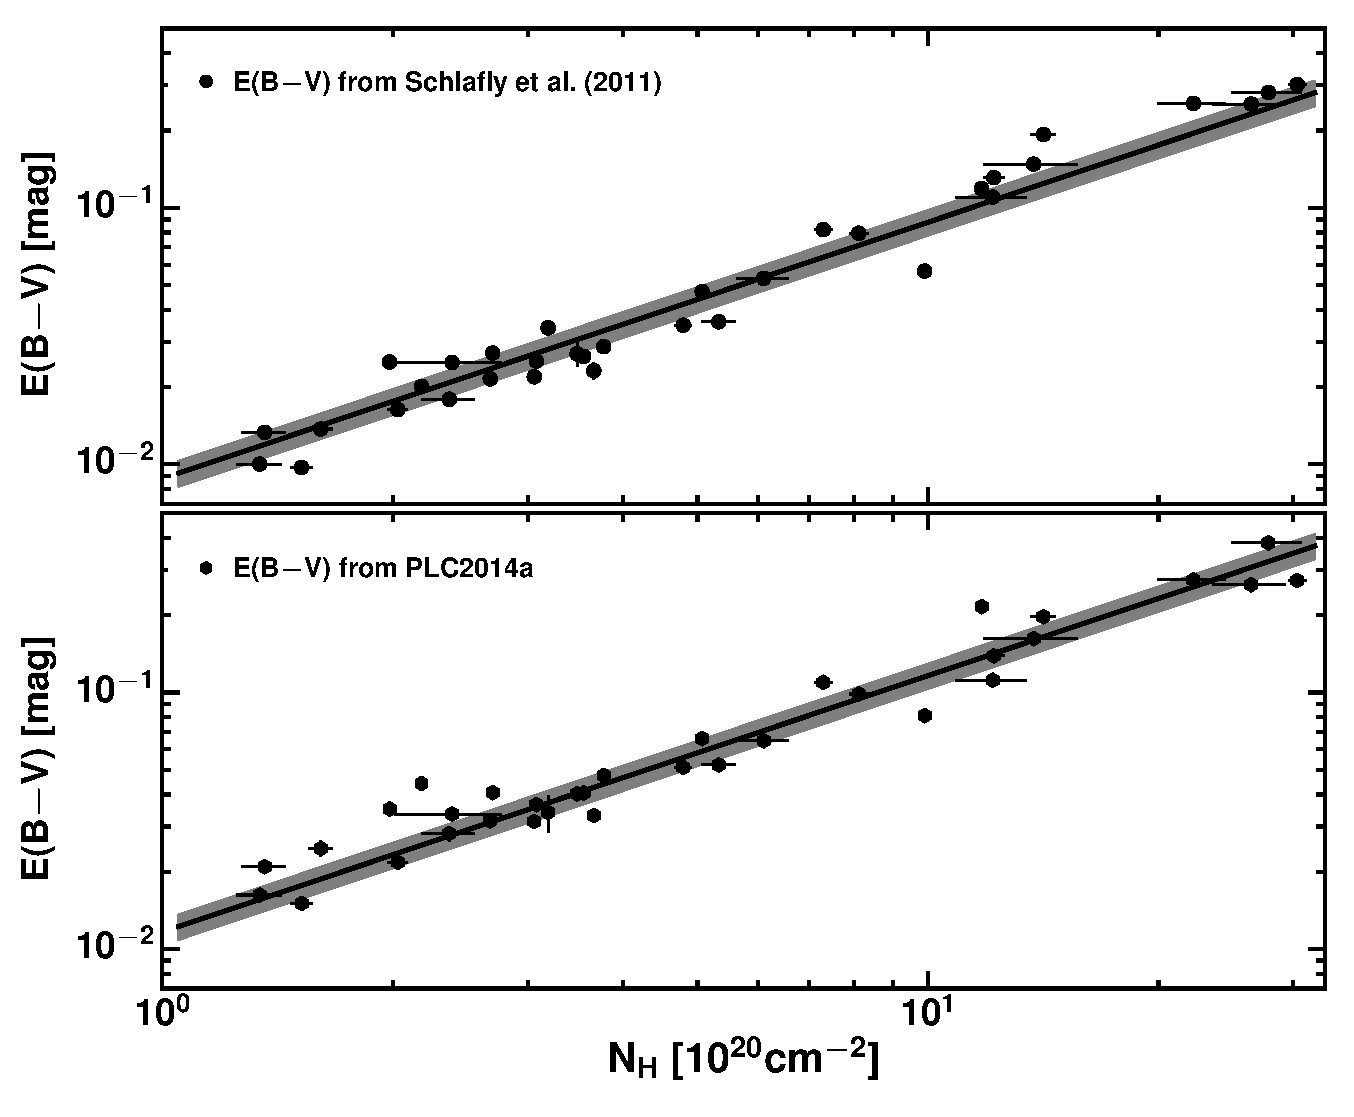
\includegraphics[width=1.0\linewidth]{fig/ebv_vs_nh.eps}
\caption{Correlation between \NH\ and dust reddening \ebv\ from \citealt{Schlafly2011} (upper panel) as well as from PLC2014a (lower panel) along 35 atomic sightlines (19 sightlines without CO and OH detection and 16 sightlines with low \NHI).}
\label{fig:ebv_vs_nh}
\end{figure}

For completeness, we also perform the same analysis using the \ebv$_\mathrm{xgal}$ map presented by PLC2014a (Release 1.2), which is a scaled version of their map of \rad. The results are plotted in the lower panel of Figure \ref{fig:ebv_vs_nh}. Here, the derived \NH/\ebv\ ratio is (8.6$\pm$0.3)$\times$10$^{21}$cm$^{-2}$mag$^{-1}$ \textbf{\color{magenta}[Uncertainties?]}. {\color{magenta} Similarly to our scaling of \NH\ and \rad,} this corresponds to a factor of 1.08 times higher than the value of \NH/\ebv=(6.8$-$7.0)$\times$10$^{21}$cm$^{-2}$mag$^{-1}$ obtained by PLC2014a, but is consistent to within the errors. \textbf{\color{magenta}[Check whether it really is!]}
%OK... so. They derive E(B-V) from quasars and do a scatter plot vs R to get how to scale to that. Then they can just apply their R vs NH scaling to get E(B-V)/NH. So they're using NH from R. We're using scaled-R vs our NH. So shouldn't we be consistent with them as we were for R? 

\subsection{ Evolution of dust grains from \s353}
\label{subsec:evolution-of-dust}
Many efforts have been undertaken using the correlation between \t353 and \NH, particularly with regards to the search for Dark Gas \citep[e.g.][]{PLC2011, Fukui2014, Fukui2015, Reach2015}. It is clear that \t353 and \NH\ are {\color{magenta} in general} linearly correlated only if \s353 is a constant. {\color{magenta} However, it is widely recognised that \s353 is sensitive to grain evolution, and significant variations in the ratio \NH/\t353 have been observed, particularly when transitioning to the high-density, molecular regime \citep[e.g.][]{PLC2014, PLC2015, Okamoto2017, Remy2017}.} The origin of observed variations in \s353 may relate to a change in dust properties via $\kappa_{0}$, but may also include a contribution due to the presence of Dark Gas, {\color{magenta} if this is unaccounted for in the estimated \NH}. PLC2014a measured the variation in \s353 with \NH\ {\color{magenta} at 30$'$ resolution over the entire sky, where their \NH\ is derived from (\NHIthin\ + $X_\mathrm{CO}W_\mathrm{CO}$).} We reproduce their data in Figure \ref{fig:s353_vs_nh}. It can be seen that \s353 is roughly flat and at a minimum in a narrow, low-column density range \NH=(1$-$3)$\times$10$^{20}$cm$^{-2}$, then increases linearly until \NH=15$\times$10$^{20}$cm$^{-2}$, by which time it is almost a factor of 2 higher. {\color{magenta} After this point, it remains approximately constant for the canonical value of \xco=$2.0\times10^{20}$cm$^{-2}$K$^{-1}$km$^{-1}$s. The pertinent issue for Dark Gas studies is disentangling how much of this apparent change in \s353 is due to changing grain properties, and how much is due to the contribution of unseen material (whether it be opaque \hi\ or diffuse H$_2$).}
Fortunately, the column density range probed by our purely atomic sightlines, \NH=(1$\sim$30)$\times$10$^{20}$cm$^{-2}$ ($A_V\sim$??--??) well samples the range where \s353 undergoes its first linear increase. This allows us to explore its origin, {\color{magenta} at least in the atomic regime}.% the dark gas hypothesis versus the dust properties one. %\sout{[JO NOTE: Probably good to describe here efforts that have been undertaken using this relationship, particularly with regards to the search for ``dark gas''. This is a good place to contrast Fukui's treatment with others, and mention something about the range of sigma values, and the change in sigma with \hi column that was observed by Marc-Antoine. State that the origin of variations in sigma may be dust properties (Marc-Antoine could advise on an appropriately sophisticated explanation), but may also include a dark gas contribution. State that our column density range overlaps with the place where deviations begin to be seen, hence we are in a position to test the dark gas hypothesis vs the dust properties one.]}

\sout{To understand the reason why we have the fluctuation of data points out of the linear trend, especially, the systematic offset above the best fit line at higher column densities %\sout{[JO NOTE: ``scattering'' may not be the best word. You mean the systematic offset above the best fit line at higher columns, right?]} 
as seen in Figure \ref{fig:tau_vs_nhi}, we also} 
We compute dust opacity \s353\ for each of our sightlines using Planck \t353\ data and our opacity-corrected \hi\ column densities. %\textbf{\color{red}[JO (16/6/17): This is sort of repetitious now - we have already discussed the offset above, and indeed expect to see it. And it would probably be trivial to mention the numerical value of our $\sigma_{353}$ when we initially present the linear correlation above. Therefore I think some minor reorganisation is required]}. 
Figure \ref{fig:s353_vs_nh} shows \s353\ as a function of \NH\, superimposed on the results from PLC2014a. It can be seen that we observe a similar rise in \s353 in the column density range of (5$\sim$30)$\times$10$^{20}$cm$^{-2}$.

\begin{figure}
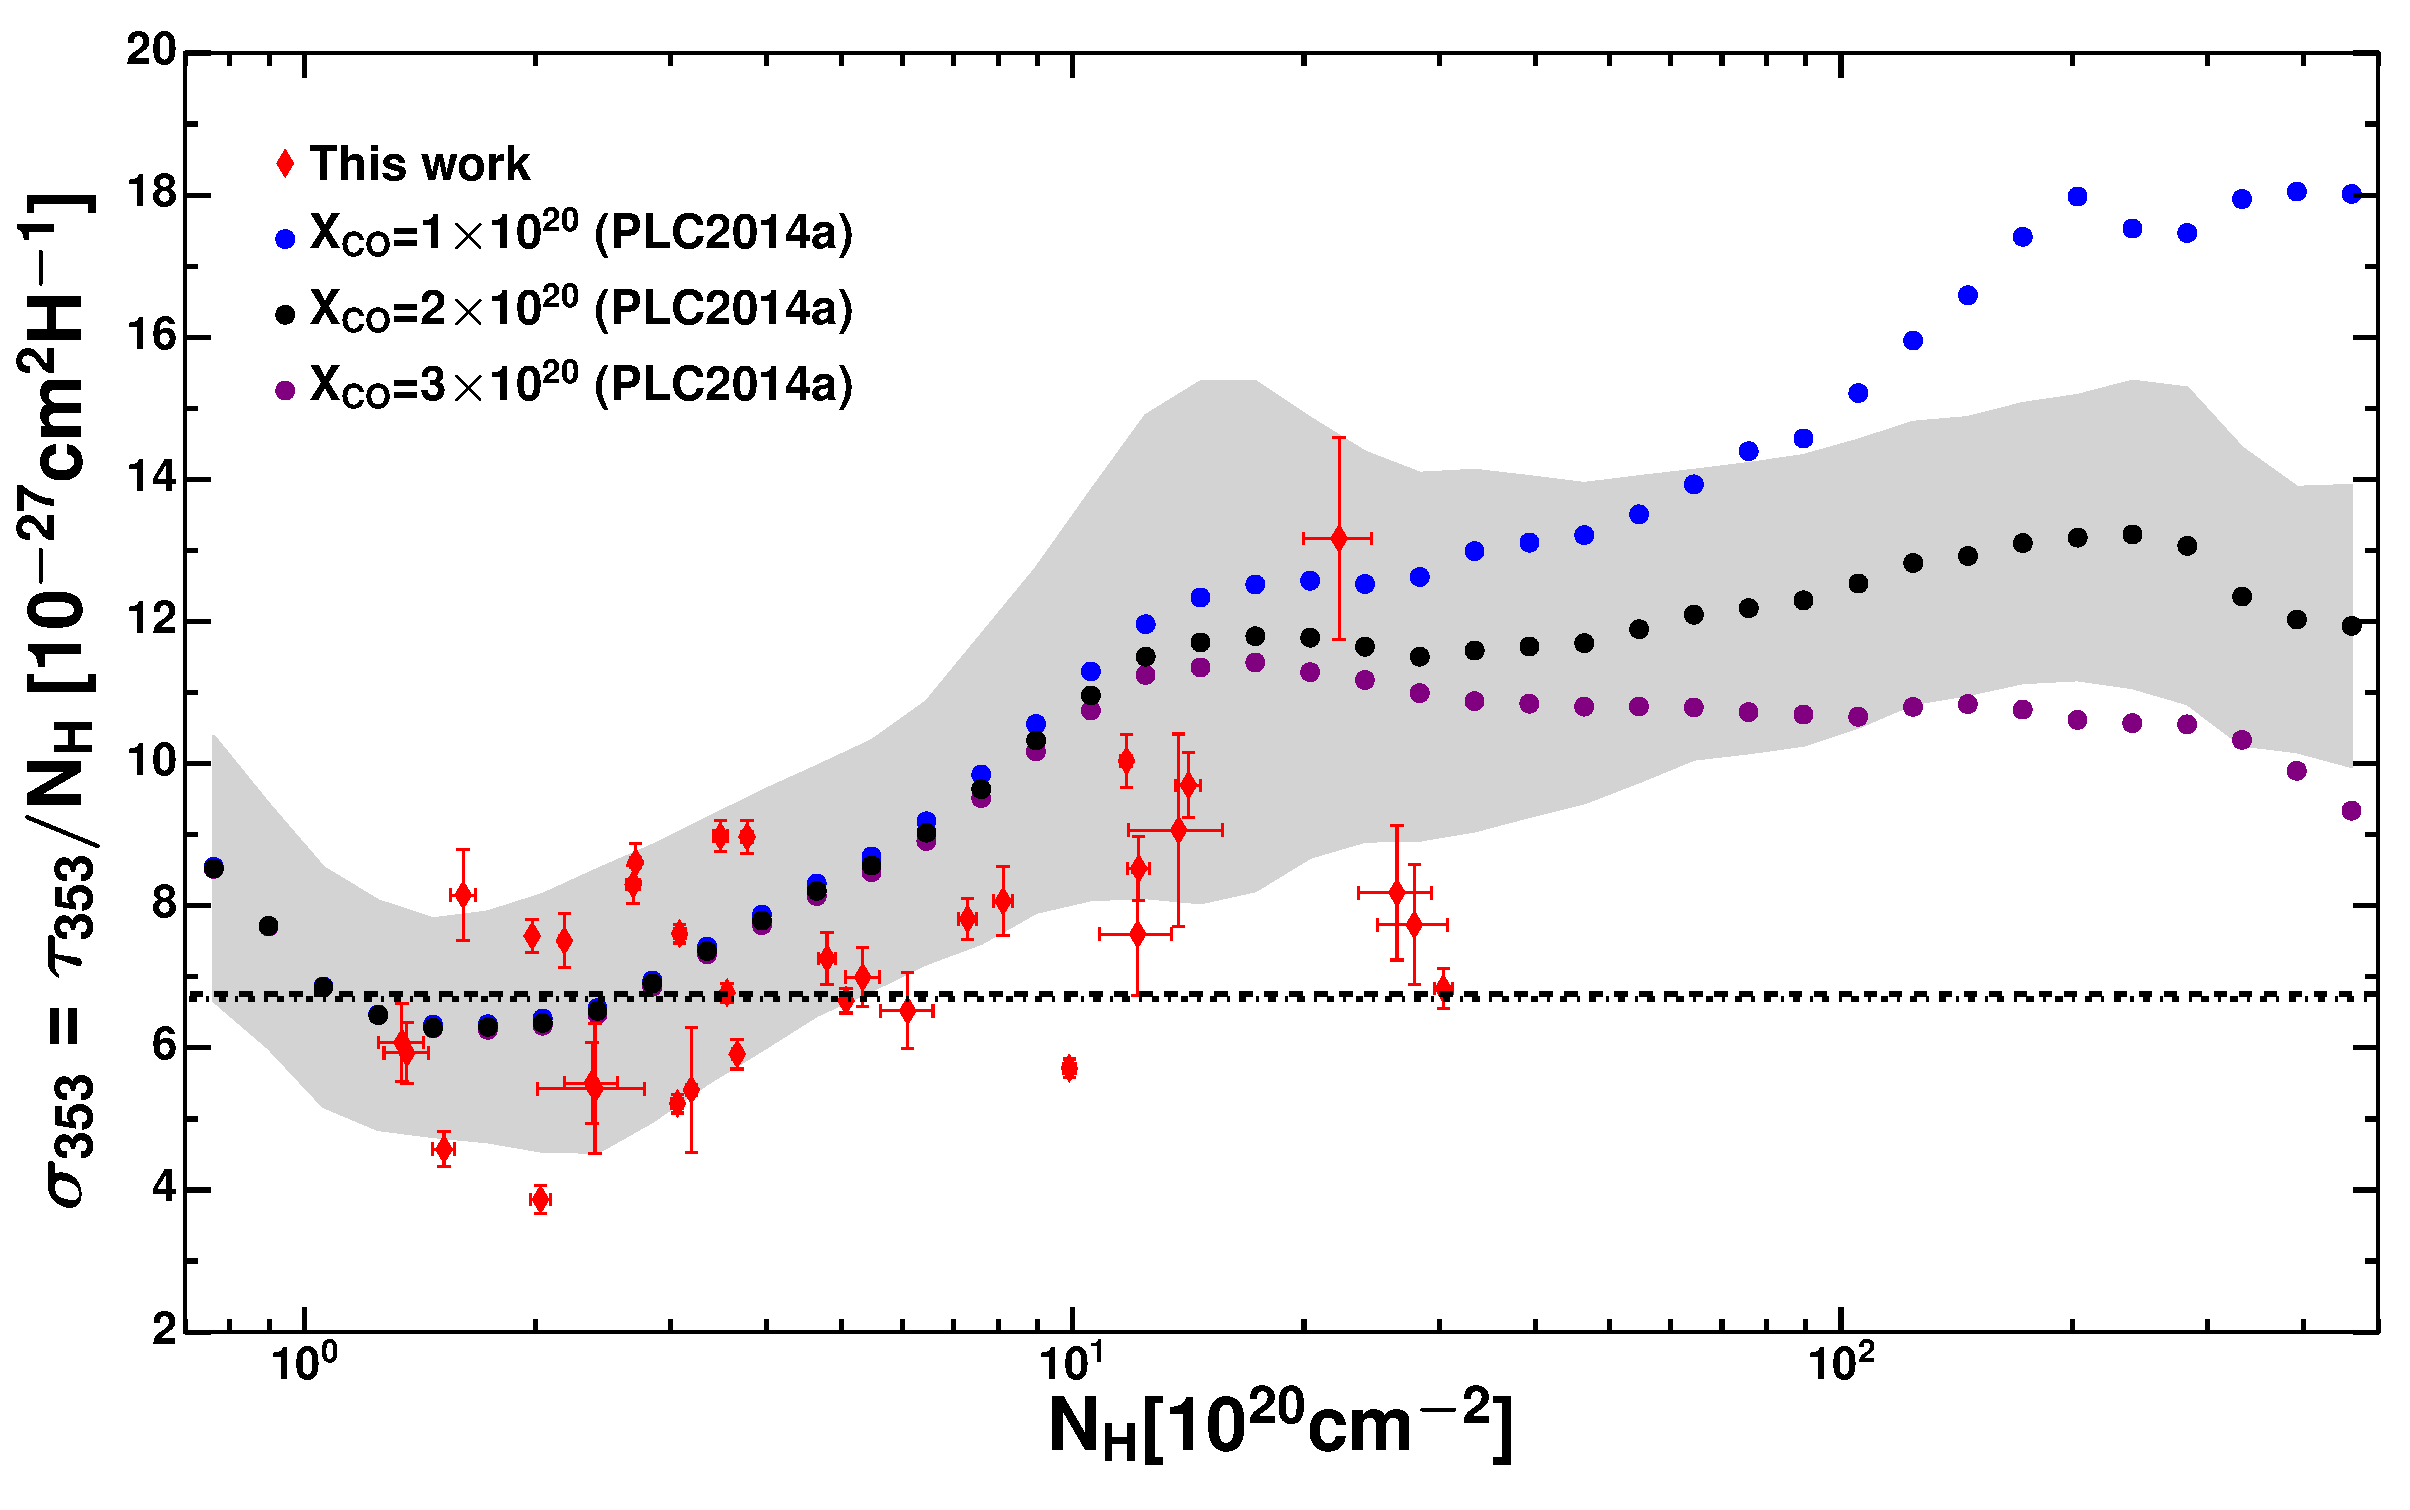
\includegraphics[width=1.0\linewidth]{fig/sig353_vs_nh.eps}
\caption{Dust opacity \s353 versus total column density \NH\ (red) along 35 atomic sightlines. \s353 at 30$'$ resolution from PLC2014a within the same \NHI\ range is superimposed, blue for CO X-factor \xco=1.0$\times$$10^{20}$, black for \xco=2.0$\times$$10^{20}$ and violet for \xco=3.0$\times$$10^{20}$. Dot-dashed horizontal line represents the average value of dust opacity $<$\s353$>$ found in low \NHI\ mask, (1$-$4)$\times$10$^{20}$cm$^{-2}$, dashed line for $<$\s353$>$ from PLC2014a.}
\label{fig:s353_vs_nh}
\end{figure}

{\color{magenta} Since our sample of purely atomic sightlines by definition includes no Dark Gas, the observed increase in \s353 must arise due to changes in dust properties.} From equation \ref{eq_t353_nh}, {\color{magenta} we see that \s353 is a function of} $\kappa_{0}$, the dust emissivity cross-section, which depends on the composition and structure of dust grains. Because $\kappa_{0}$ is the ratio of the extinction cross-section over the dust mass \textbf{\color{magenta} [``grain mass''??]}, %it depends on size of large grains. $\kappa_{0}$ of a dust grain 
it is inversely proportional to grain size. %the bigger grain would have smaller $\kappa_{0}$. 
But \cite{Kohler2012} claim that during the coagulation of particles into fluffy dust grain (or ``Grain-grain coagulation into fluffy aggregates''), $\kappa_{0}$ apparently increases by a factor of 2--3 for silicate grains with the size range relevant of the ISM \textbf{\color{magenta} [Over what change in density?]}. Thus, the rise in \s353 seen in Figure \ref{fig:s353_vs_nh} in both our data and PLC2014 %are due to the 
is well explained by an increase in the emission cross-section $\kappa_{0}$. \textbf{\color{magenta} [Jo note: Need to review this text so that it doesn't sound like we're just relying on this one result and its factor of 2--3 finding. There should be a larger body of literature backing us up.]}
The other factors are either constants or slightly change. \textbf{\color{magenta} [Expand briefly here on why $r$ won't change much.]}%\textbf{\color{magenta} [Do you mean m$_H$, $\mu$ and $r$? Presumably $r$ is the only one of these that can change? Should probably state this explicitly. e.g. ``The other variable, $r$, the dust-to-gas mass ratio, is generally assumed to show minimal variation outside of dense molecular regions.''. I added this last comment about molecular clouds based on Tricco et. al. (2017), which I just found via Google. But honestly, I don't really know if the statement is true...]} 
%{\em The total gas column densities are indeed the true column densities of \hi\ along atomic sightlines.} 
%Thus, we can explain that the \textbf{scattering/fluctuations ???} seen in Figure \ref{fig:tau_vs_nhi} are due to the variation of the emission cross-section $\kappa_{0}$ %[because $\kappa_{0}$ is the division of extinction cross-section over the dust mass, it depends on size of large grains. $\kappa_{0}$ of a dust grain is inversely proportional to its size, the bigger grain would have smaller $\kappa_{0}$. But \cite{Kohler2012} claim that during the coagulation of particles into fluffy dust grain (or "Grain-grain coagulation into fluffy aggregates"), $\kappa_{0}$ apparently increases by a factor of 2-3 for silicate grains with the size range relevant of the ISM]. 

The rise seen in Figure \ref{fig:s353_vs_nh} is \sout{explained by} {\color{magenta}thus interpreted as the effect of} dust evolution from a lower column density to higher column density regime. \textbf{\color{magenta} [This paragraph should maybe comment on things like: the fact that we are seeing this evolution for purely atomic sightlines, that we don't have a perfect proxy for true gas density since we're generally collapsing a number of gas components along the line of sight... etc. Ideally we should be able to argue that the proposed rise in $\kappa_0$ is consistent with WNM to CNM transition (as opposed to CNM to H$_2$). Once the figure has been replotted with the updated sample and new NHI values, we should perhaps speculate on why all (?) our points lie below the Planck trend? Something to do with the fact that we're tending to sample smaller n$_H$ since we're only looking at atomic gas? Planck sample would have had molecular gas in these bins too, presumably with a higher $\kappa_0$ etc?]}
%This rising of \s353\ is truly existing and is not caused by any unaccounted dark gas.

%  \sout{Denser gas leads to higher dust density, dust grains collide to each other more frequently, small dust grains stick onto the surface of bigger dust grain through coagulation, hence the total surface area of the final dust grain increases. Since the dust emission in sub-mm range originates mostly from bigger dust grains in thermal equilibrium with the ambient radiation field; moreover, the emission capability of any object depends on its total area and controversially its absorption capability is proportional to the projected area perpendicular to the direction of coming-radiations, larger surface area enhances the emission cross-section $\kappa_{0}$ of dust grain.} 

\subsection{ Possible presence of ``dark gas''}
\label{subsec:possible-dark-gas}

Follow the PLC2014a, we also plot in Figure \ref{fig:lh_vs_nh} the dust specific luminosity \LH=4$\pi$\rad/\NH\ as the function of \NH. Both data sets show that \LH\ decreases/drops where \NH$<$1.2$\times$10$^{20}$cm$^{-2}$ and keeps roughly constant at a minimum in small range 1.2$\times$$10^{20}$$<$\NH$<$3$\times$10$^{20}$cm$^{-2}$. However, while they see the rise of \LH\ from $\sim$3.2$\times$10$^{-31}$ to $\sim$4.5$\times$10$^{-31}$WH$^{-1}$ in column density range (3$-$15)$\times$10$^{20}$cm$^{-2}$ then the drop of \LH\ from 5$\times$10$^{-31}$ to 3$\times$10$^{-31}$WH$^{-1}$ in the range \NH=(15$-$50)$\times$10$^{20}$cm$^{-2}$, we notice that it is still constant (red data points). Because we consider sightlines containing only \hi, this means (/meaning) that their shape of the deviation of \LH\ within gas column densities from (3$-$50)$\times$10$^{20}$cm$^{-2}$ can be explained by (1) the presence of ``dark gas'' or (2) the change in G$_{0}$. \sout{\color{red}[JO NOTE: I removed my incomplete text here. Just a note that this explanation needs to be crystal clear and also well backed up by whatever text has preceded this part of the paper.]}

\begin{figure}
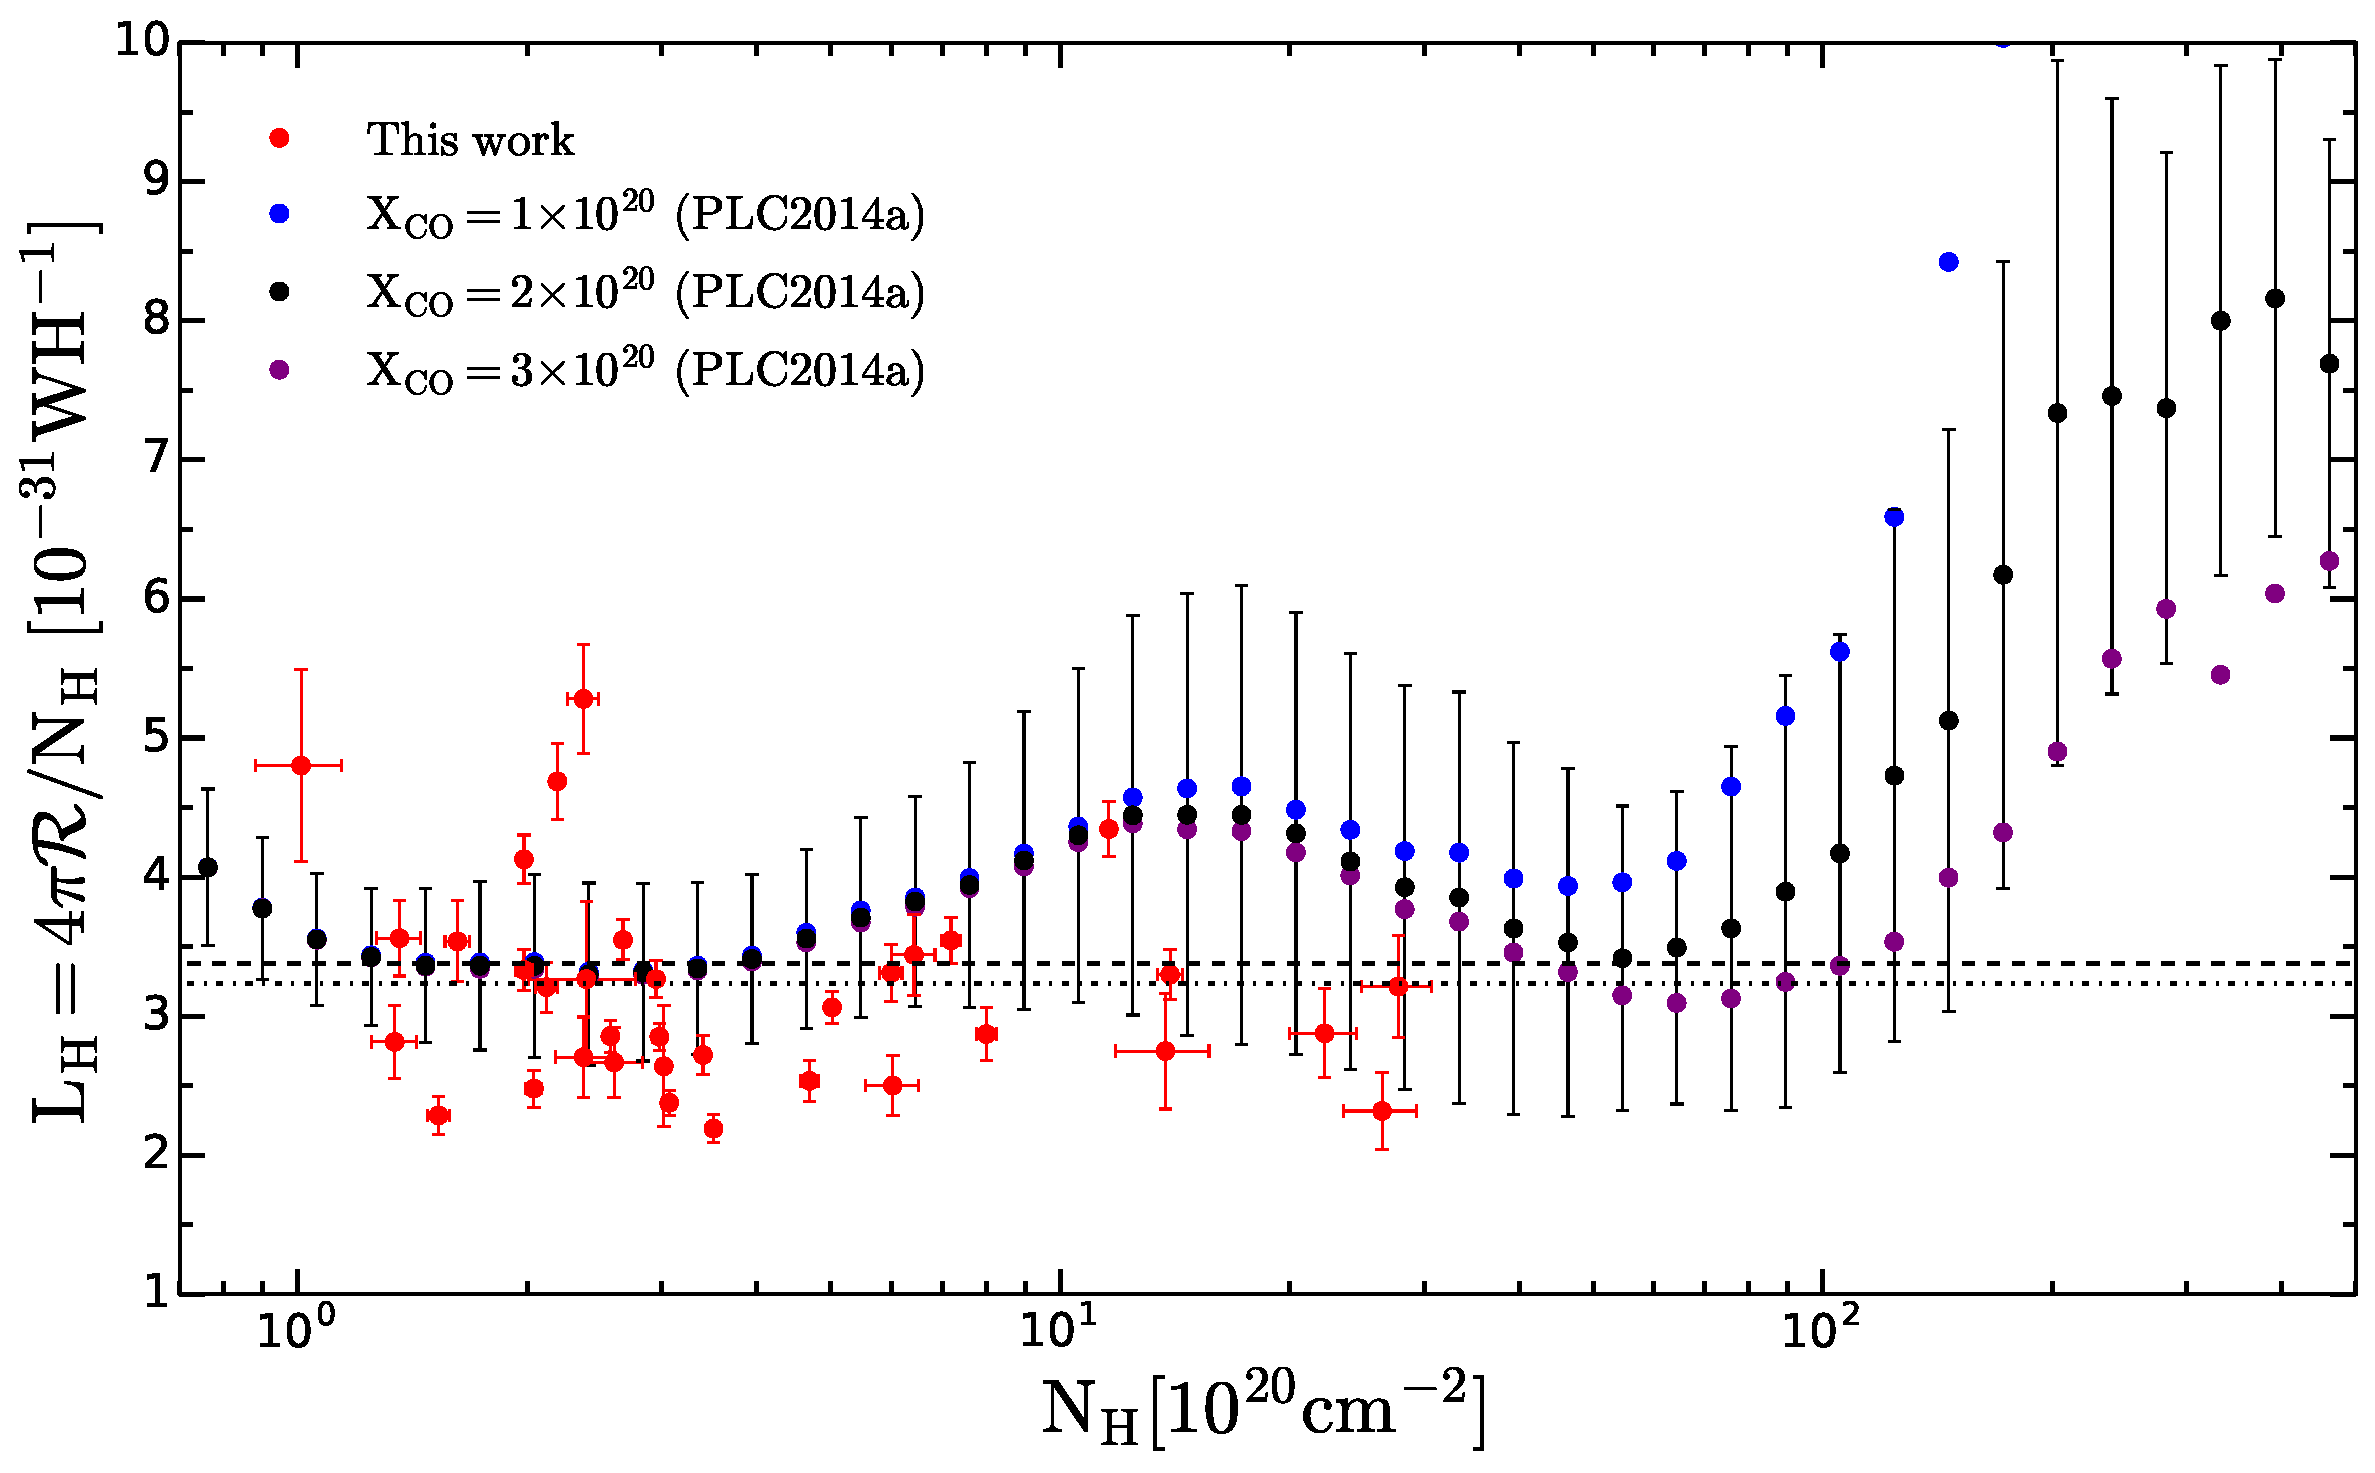
\includegraphics[width=1.0\linewidth]{fig/LH_vs_nh.eps}
\caption{\LH\ vs \NH\ along 35 atomic sightlines. \LH\ computed at 30$'$ resolution from PLC2014a is also superimposed, blue for CO X-factor \xco=1.0$\times$$10^{20}$, black for \xco=2.0$\times$$10^{20}$ and violet for \xco=3.0$\times$$10^{20}$. Dot-dashed horizontal line represents the average value of $<$\LH$>$ found in low \NHI\ mask, (1$-$4$)\times$10$^{20}$cm$^{-2}$, dashed line for $<$\LH$>$ from PLC2014a.}
\label{fig:lh_vs_nh}
\end{figure}

But it is worth noting that the ``hump'' shape in Figure \ref{fig:lh_vs_nh} from PLC2014a data is seen in the range of \NH=(3$-$50)$\times$10$^{20}$cm$^{-2}$, corresponding to the visual extinction \av\ from (0.17$-$2.78) mag and peak at \NH$\sim$15$\times$ 10$^{20}$cm$^{-2}$ (or \av$\sim$0.8 mag). This \av\ range is consistent with the \av\ range where ``dark gas'' can be observed (\citealt{PLC2015}): if \av\ is low, \h2\ is destroyed by UV photo-dissociation and in high \av\ regions, CO can be formed and therefore \h2\ would be traced by CO, the peak is found at \av$\sim$0.8 mag where \h2\ has already formed and achieved self-shielding but CO has not formed. \LH\ then increases massively after the hump because the radiation field intensity, $G_0$, increases due to the effective contribution from star forming regions at high column densities.
% This could indeed be another [NEED TO CHANGE TEXT HERE] convincing evidence for dark gas, and in some extent we can use dust specific luminosity (or dust radiance) to trace the dark gas  in the ISM.

In the case the ``hump'' of \LH\ in  \av=(0.17$-$2.78) mag is due to ``dark gas'': 35 atomic sightlines (red points) contain \hi\ only with $<$\LH$>$$\approx$3.2$\times$10$^{-31}$WH$^{-1}$, as we assume \rad\ and \NH\ linear correlate (\LH\ = constant), this means every single H atom corresponds to an amount of $\sim$3.2$\times$10$^{-31}$W; \LH\ at the peak is $\sim$4.5$\times$10$^{-31}$W meaning that we need $\sim$1.4 H atoms or 40\% more H atoms. Since the ``hump'' is symmetry, the amount of ``dark gas'' is approximately 20\% of measured \hi\ in \av\ range (0.17$-$2.78) mag (CONSISTENT? REFs?  (Grenier et al 2005, Planck collab.
2011 XIX) ).

\cite{PLC2015} used $\gamma$ rays from Fermi LAT as the proxy for \NH\ to study the case of Chamaeleon clouds. They also notice a consistent decrease of \LH\ from 5$\times$10$^{-31}$ to 3$\times$10$^{-31}$WH$^{-1}$ in \NH\ range of (8$-$50)$\times$10$^{20}$cm$^{-2}$. It is clear that the maximum value of \LH\ in this case is slightly shifts to lower \NH. This is probably because they derived total \NH\ from $\gamma$ rays for specific molecular clouds while total \NH\ in PLC2014a is calculated from optically-thin \hi\ and CO data for the all-sky scale.

Since dust grains are in thermal equilibrium with the ambient interstellar radiation field, \rad\ is simply equal to the amount of energy absorbed (or emitted) by dust and it does not either depend on the shape of spectral energy distribution (SED) or the dust cooling efficiency. \sout{I would simplify the following sentence by saying that CIBA is a lesser contaminant in $R$ compared to $\tau_{353}$ and simply refer to the Planck paper.} In addition, \rad\ is less contaminated by the Cosmic Infrared Background Anisotropies (CIBA) compared to \t353 (PLC2014a). \sout{[JO NOTE/state: Probably need either more or less explanation here. i.e. Either define CIBA and explain more of the basics, or omit.]}, the 3 factors in equation \ref{eq_r_nh} dust-to-gas ratio $r$, absorption cross-section $\sigma_{a}$ and radiation field intensity $G_{0}$ do not widely vary. \LH\ fluctuates only in a narrow range ($\sim$2$-$3.5)$\times$10$^{-31}$WH$^{-1}$, thus dust radiance \rad\ is not scattered extensively away from the linear relationship with \NH\ as seen in Figure \ref{fig:r_vs_nh}. \sout{[JO EDIT: Suggest demonstrating this lack of scatter explicitly in a similar plot to Fig 6. Also, commenting on the significance - Radiance is a better proxy than tau? (Consistent with Planck 2014?)]} 

We have so far seen that along 35 atomic sightlines: \ebv\ and \rad\ have tight linear relations with \NH\ in the \av\ range 0.03$\sim$1.5 mag; \t353\ also has a linear relation with \NH\, but begins to deviate towards top end of this \av\ range. Unfortunately, we do not have opportunity to understand how these relations will change when approaching higher \av\, as well as regimes of molecular clouds. Yet we could be sure \t353\ is far from the linear relation with \NH.

As we discussed earlier, \t353\ is a parameter derived from a MBB fit. It is contaminated by the CIBA because it is the quotient of $I_{353}$ and the Planck function $B_{353}(T_{obs})$. \t353 is proportional to \NH\ only if \s353 is constant, but \s353 largely varies in low-to-moderate \NH\ due to the dependence of \t353 on dust emissivity cross-section $\kappa_{0}$. Meanwhile, dust radiance \rad\ seems to be a measurable quantity and it correlates with \NH\ in wider range. This suggests that radiance could be a better proxy for \NH\ than \t353 in low-to-moderate \NH\ range. Indeed, along all 94 sightlines considered in this work, the ratio between \NH\ obtained from \t353 and from radiance increases and reaches the factor of 4 as visual extinction \av\ rises fro 0.03 to 4.8 mag, whereas that ratio from \ebv\ does not seem to exceed the factor of 2 (see Figure \ref{fig:ratios_of_nh}).

\begin{figure}
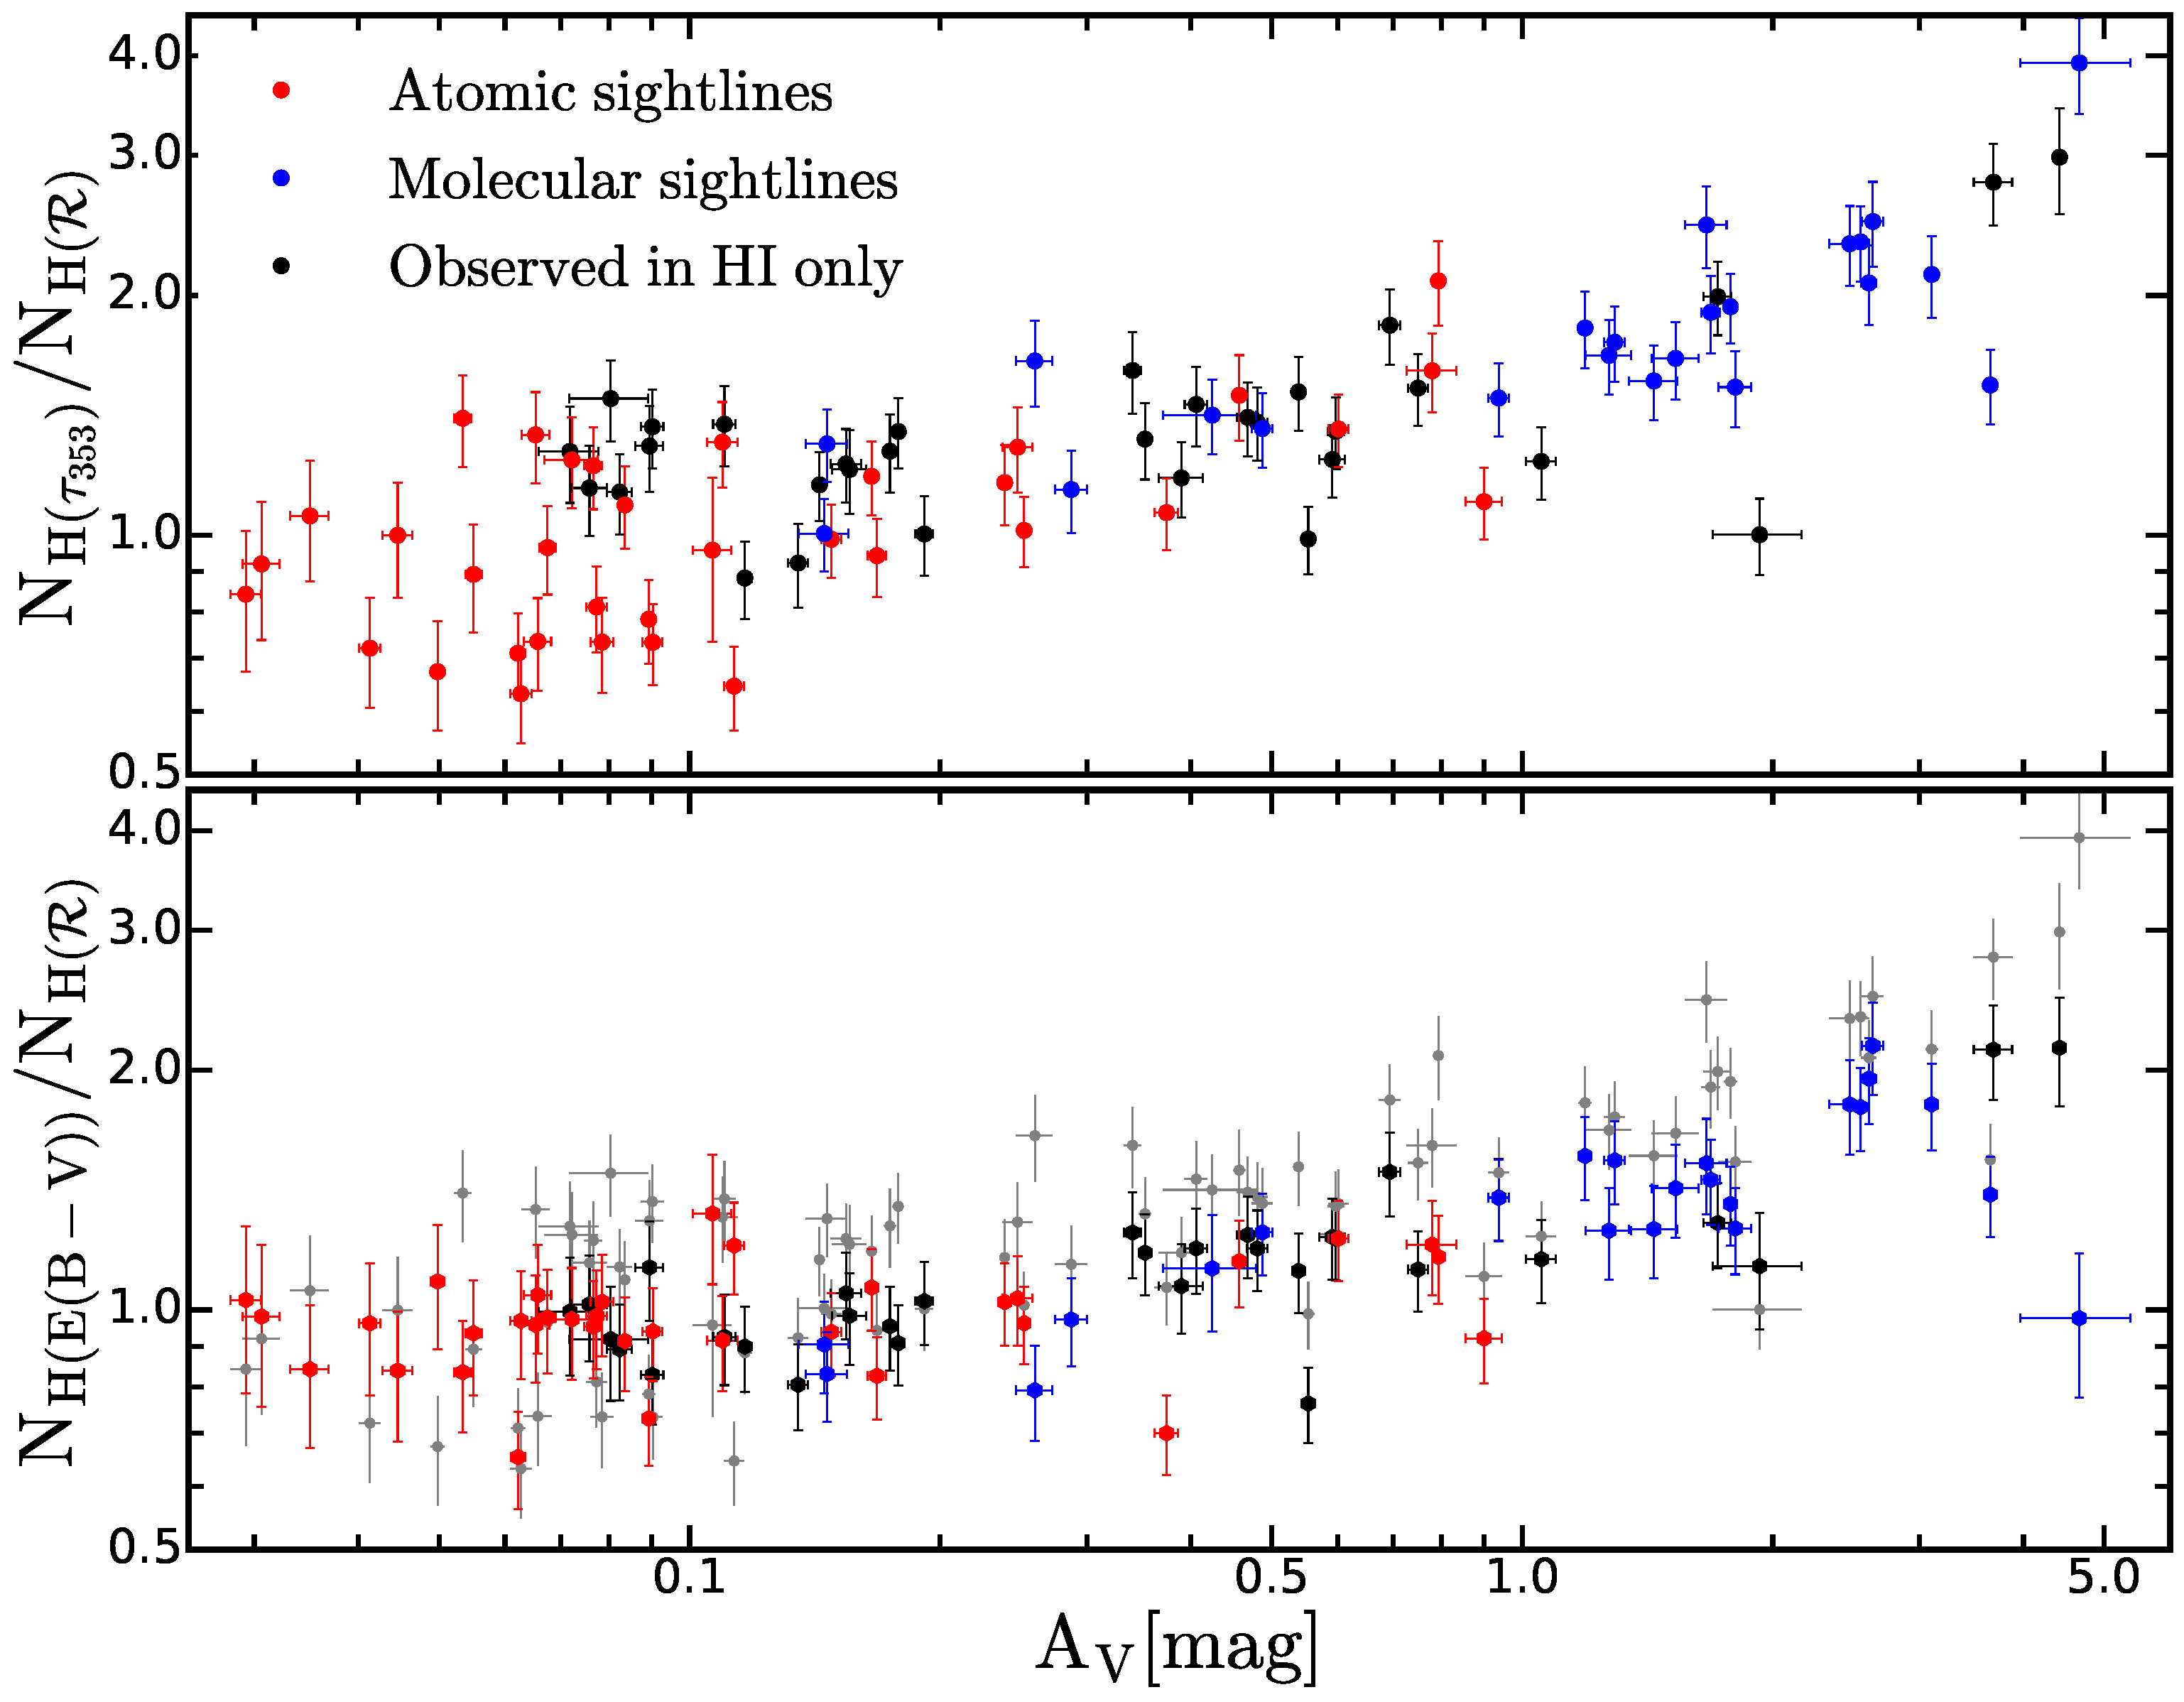
\includegraphics[width=1.0\linewidth]{fig/ratios_of_NH.eps}
\caption{Comparison of \NH\ obtained from \t353, \ebv\ and \rad\ along 94 sightlines: Ratios $N_{H(\tau_{353})}/N_{H(\mathcal{R})}$ (upper) and $N_{H(E(B-V))}/N_{H(\mathcal{R})}$ (lower) as the function of \av. Red for 35 atomic sightlines; blue for molecular sightlines (CO or OH detection); black for sightlines observed in \hi\ only, not observed in either CO or OH. Grey points in lower panel are those from upper panel for comparison purpose.}
\label{fig:ratios_of_nh}
\end{figure}

\section{OH abundance ratio \xoh}
\label{sec:xoh}
The 2.6mm emission line of CO has been used to probe the physical properties of \h2 clouds, but in the regimes where CO is not detectable, other molecular/atomic transitions (e.g OH ground state main lines at 1665 and 1667MHz, CH ground state main line at 3335 MHz, ortho $1_{10}$-$1_{01}$ and para $2_{20}$-$2_{11}$ transitions of C$_{3}$H$_{2}$ at 18.3 and 21.6 GHz, $^3$P$_1$$\rightarrow$$^3$P$_0$ fine structure line of atomic carbon at 492 GHz, etc.) have been considered as potential alternative tracers of \h2. However, it is worth noting that \cite{Cotten2013} claimed CO(1-0) observations at higher sensitivity (greater than the 0.1-0.2 K rms) can trace molecular gas in regions where \av$\sim$0.3 mag. Among these alternatives, the ground-state main lines of OH are the easiest to observe; they are readily detectable in translucent/diffuse molecular clouds (\citealt{Magnani1990}, \citealt{Barriault2010}), OH is considered as a precursor molecule necessary to the formation of CO in diffuse regions (\citealt{Black1977}, \citealt{Barriault2010}), and thus it is expected to be abundant in low CO density/abundance regimes.

To estimate the \h2 column density from OH, we have to determine the OH abundance ratio with respect to \h2, \xoh= \NOH/\NHm. 

Many efforts (models or observations) have been devoted to derive \xoh\ in different environment conditions:

% - Models of translucent and diffuse molecular clouds with \av\ from 0.1 to 1 mag and $T_{K}$ from 50 to 100K by Viala (1986) found that the \xoh\ varied from 3.8$\times$10$^{-9}$ to 9.4$\times$10$^{-9}$. 

- Astrochemical model by \citet{Black1977} shows that \xoh$\sim$$10^{-7}$ for the case of $\zeta$ Ophuichi cloud.

- 19 comprehensive models of diffuse interstellar clouds with \nh\ from 250 to 1000 \cc, $T_{K}$ from 20 to 100K and \av\ from 0.62 to 2.12 mag \citet{vanDishoeck1986} found OH/\h2\ abundances from 1.6$\times$$10^{-8}$ to 2.9$\times$$10^{-7}$.

- OH abundance with respect to \h2\ from chemical models of hot diffuse cloud and moderate diffuse cloud (\citealt{Viala1986}) varies from 7.8$\times$$10^{-9}$ to 8.3$\times$$10^{-8}$ with \av=(0.1$-$1)mag, $T_{K}$=(50$-$100)K, $n$=(50-1000)\cc.

- 6 model calculations (that differ in depletion factors of heavy elements and cosmic ray ionization rate) by \citet{Nercessian1988} towards molecular cloud in front of star HD 29647 in Taurus show that OH/\h2\ ratio extend from 5.3$\times$$10^{-8}$ to 2.5$\times$$10^{-6}$. The best fit was obtained with \av=3.7 mag, \nh=800\cc and a uniform low temperature T=10K.

- From OH observations towards high-latitude clouds using 43m NRAO telescope, \citet{Magnani1988} derived \xoh\ from 4.8$\times$$10^{-7}$ to 4$\times$$10^{-6}$ in the range of \av=(0.4$-$1.1) mag (excitation temperatures of OH mainlines were assumed to be equal, T$_{ex(1665)}$=T$_{ex(1667)}$).

- Andersson \& Wannier (1993) obtained the OH abundance of $\sim$$10^{-7}$ from the model of halo around dark molecular clouds. Weselak et al. (2010) derived OH abundance of (1.05$\pm$0.24)$\times$$10^{-7}$ from OH absorption line observations of 5 translucent sightlines; these results are almost identical to the \xoh\ estimated by Liszt \& Lucas (2002).  

The past studies indicate that the OH abundance ratio in molecular regions varies in a wide range (4$\times$10$^{-9}$ to 1$\times$10$^{-6}$), in this paper we also determine our own OH abundance, we use observations from Arecibo telescope to provide \NOH\ and \NHI; then employ \t353, \rad, \ebv\ (along with our own conversion factors) as surrogates for $N_{H_{2}}$=$\frac{1}{2}(N_{H}{-}N_{HI})$. In this case, we examine only 17 specific sightlines where \NHm$>$0. We assume that the linear correlations (deduced from \t353, \rad, \ebv\ and \NHI\ towards 35 atomic sightlines) still hold in the regions of molecular clouds. In this manner, a direct estimates of the OH/\h2\ abundance ratio can be obtained from 3 different methods, thus allow us to intercompare/check the consistence among the derived OH abundances within a wide range of visual extinction \av\ (0.25$-$4.8 mag). \sout{\color{red}[JO NOTE: Say something about range of environmental conditions we are probing: from diffuse sightlines with no CO, to CO-rich molecular clouds. Or Av from ?? to ??]} Despite the potential for all calibration methods to deviate as moving into different physical regimes, we still find that OH/\h2\ abundance ratio is basically consistent for all methods, \xoh$\sim$10$^{-7}$. This is holding for sightlines with and without CO (e.g 3C132), as per Li et al. 2017 (in preparation).

% \sout{We see so far the strong linear correlations between \t353, $R$, $E(B-V)$ and $N_{H}$ despite of the fluctuation about the linear fit due to the evolution of dust grain properties. In this section, we will use \t353, $R$, $E(B-V)$ (along with our own conversion factors) as the proxies for the total gas columns $N_{H}$ to derive the OH abundance ratio, $X_{OH} = N_{OH}/N_{H_{2}}$ \textbf{[JO NOTE: Perhaps move this paragraph into the start of the next section?]}.}

\sout{JO NOTE: Say why it's important 
for which few literature measurements exist??.}

Nevertheless, there are differences in the 3 methods due to the overestimation of \NH\ derived from \t353 and \ebv\ compared to \NH\ from \rad\ (as indicated in Figure \ref{fig:ratios_of_nh}) along sightlines. The \xoh\ ratios from \t353 and \ebv\ are quite consistent and appear to be constants around 0.5$\times$10$^{-7}$, 1$\times$10$^{-7}$ respectively; whereas the \xoh\ deduced from \rad\ is higher and suggests a possible rapidly-increasing trend ($\sim$1 to 7$\times$10$^{-7}$) as \av\ rises from 0.25 to 2.8 mag. However, its uncertainties are huge, its mean value is \xoh$\sim$2.5$\times$10$^{-7}$. Three data points (3C123, 3C131, 3C133) with large uncertainties at \av=2.5 mag are in the Galactic plane, they seem to locate at the edges of dust clumps (as shown in Figure 16 and Figure 19 in Appendix).

Xu et al. 2016 found that across the boundary of Taurus molecular cloud the \xoh\ decreases from 8 to 1$\times$10$^{-7}$ as \av\ increases from 0.4 to 2.7 mag. This is somewhat consistent(?) with the trend of our \xoh, we take all the gas clumps along sightlines into account, they study a local molecular cloud where \h2\ contributes mostly to visual extinction, and their overabundance of OH in outer cloud region may be driven by the shock wave. 
% (DIFFERENCE. WHY????? The different environment? or the OH PRODUCTION caused by SHOCK WAVE: additional channel of OH production active, possibly due to the shock (e.g., Draine \& Katz 1986a) produced by the colliding streams. When shock waves propagate through the molecular ISM the ambient gas is compressed, heated, and accelerated.
% When temperature is above 300 K, the neutral-neutral reactions become important, which yield the overabundance of OH).

- \sout{Show some cases where no CO but OH. the plot???}

- \sout{Since these results are obtained in a wide ranges of longitude $l$ and latitude $b$ with some sightlines through the Galactic plane, it suggests that OH main lines are excellent tracers of molecular gas in ISM??????}

\begin{figure}
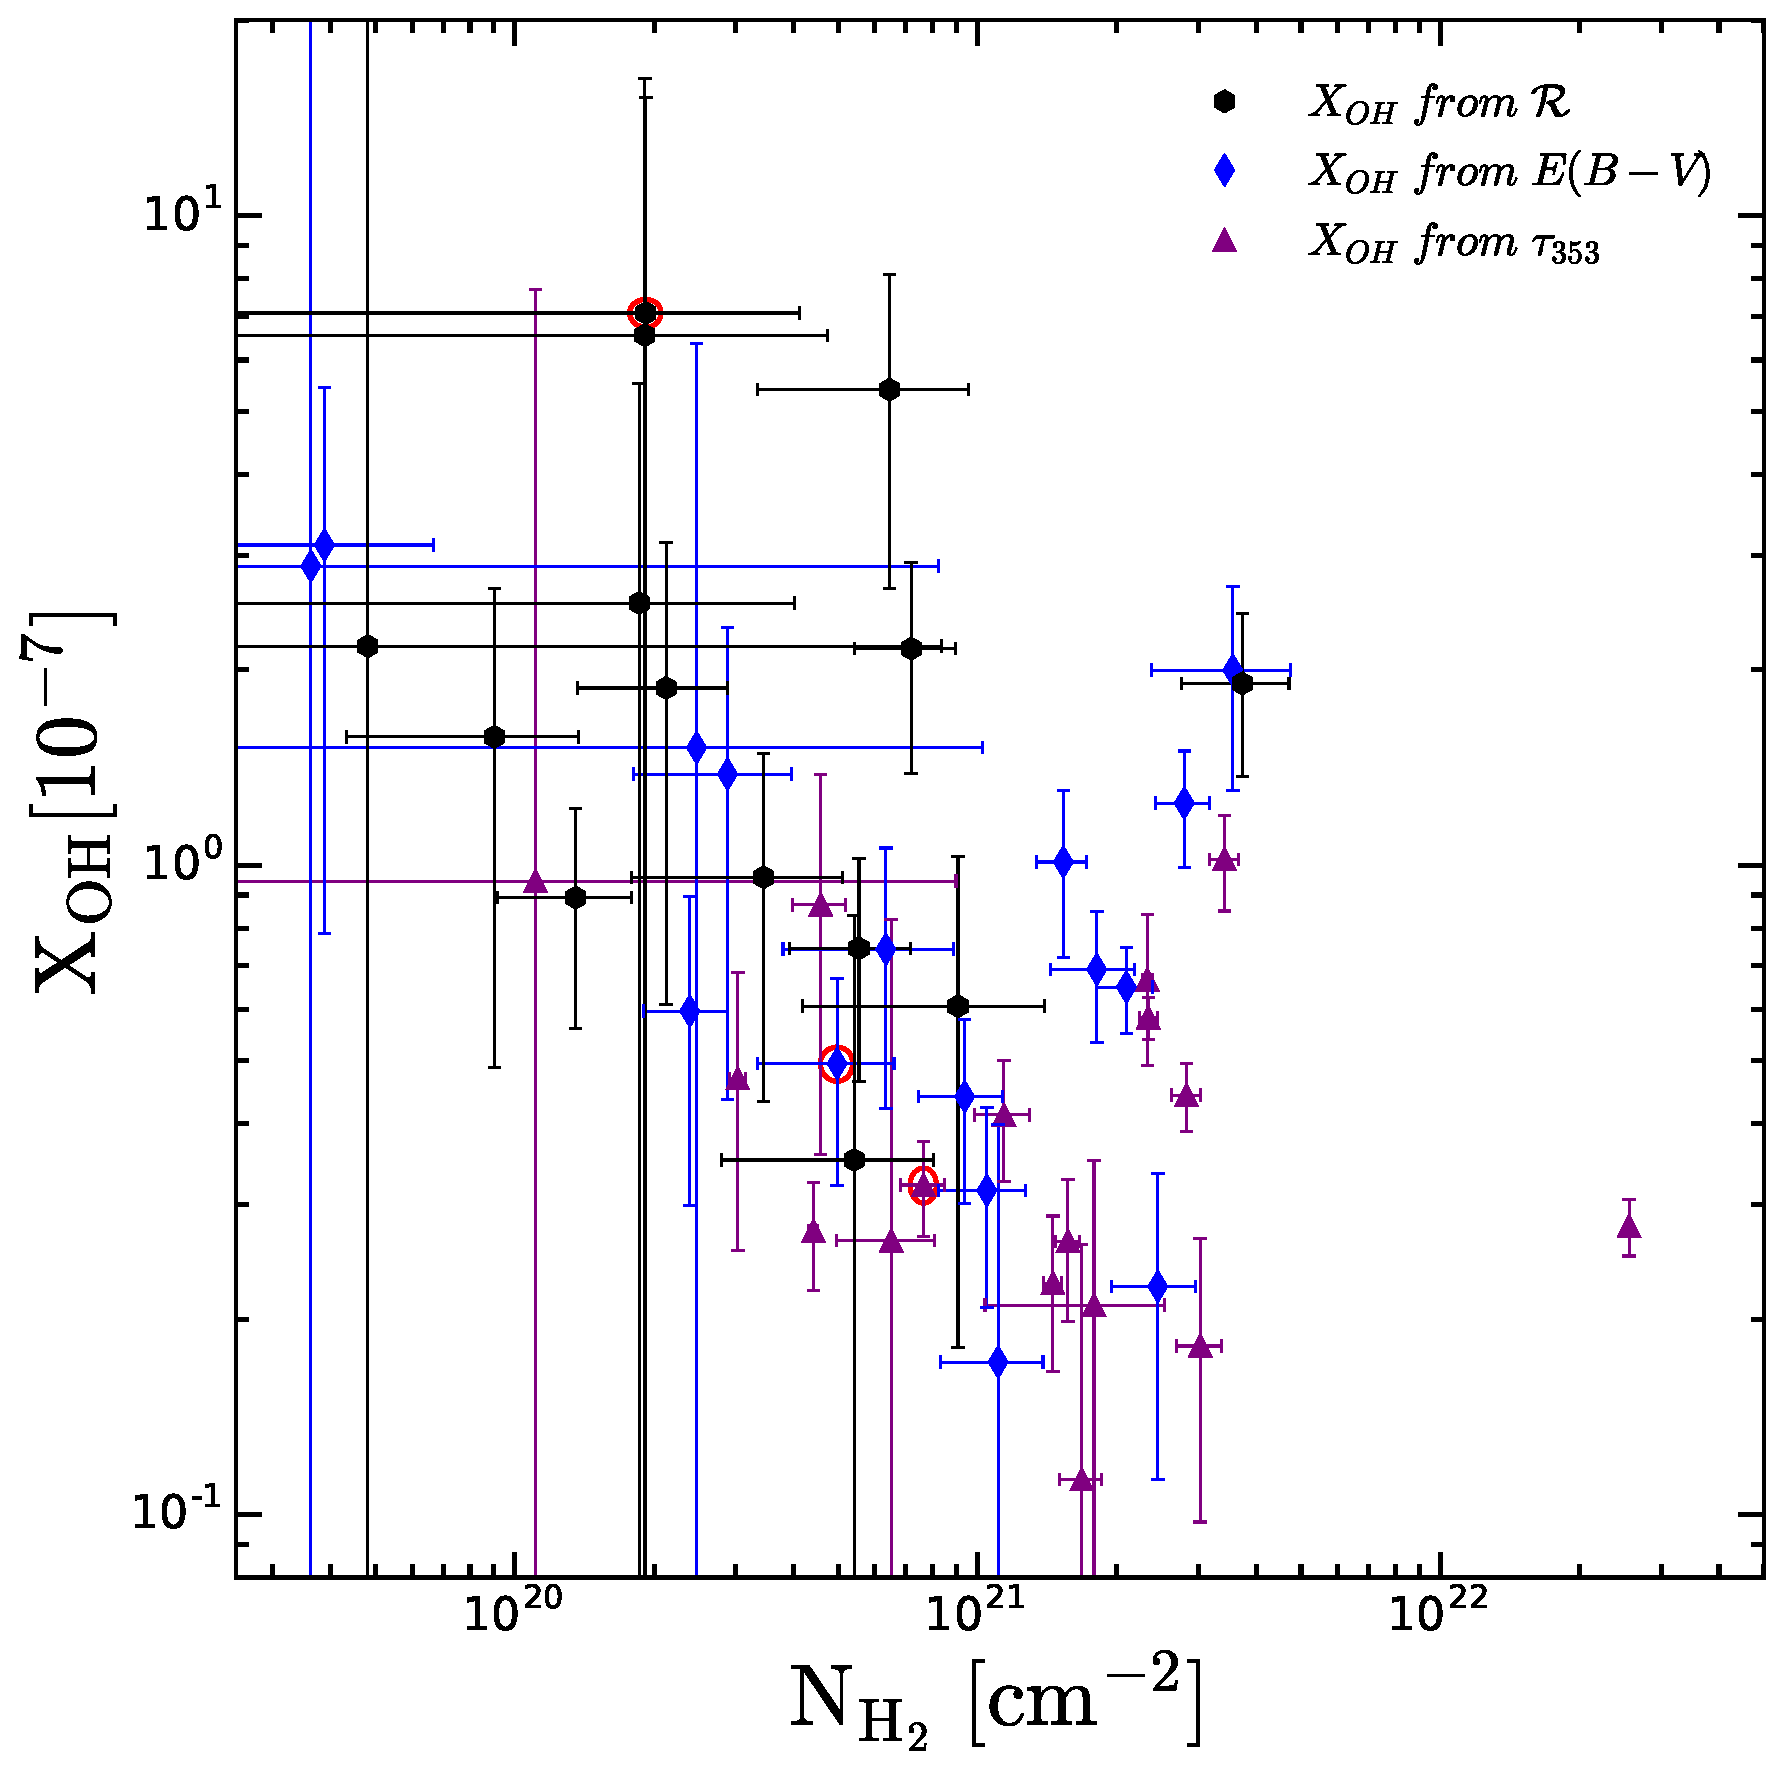
\includegraphics[width=1.0\linewidth]{fig/xoh_vs_nh2.eps}
\caption{\xoh\ derived from 3 proxies of \NH (\rad\ (black), \ebv (blue) and \t353 (red)) as the function of \NHm\ along sightlines having \NHm$>$0. OH is detected toward 3C132 (marked by red circles), but CO not detected.}
\label{fig:hist_xoh}
\end{figure}

\section{Conclusions}
\label{sec:conclusion}
The true \hi\ column densities along 94 sightlines obtained from Arecibo Millennium Survey and 21-SPONGE survey spread in a wide \sout{M.A:please quantify wide} range \NHI=(1$-$122)$\times10^{20}$cm$^{-2}$. When combining with thermal dust data from Planck collaboration and OH data also from Arecibo telescope, this gives us an excellent opportunity to reveal the possible presence of dark gas, to perceive the evolution of dust grains in different environment, as well as to estimate the OH/H$_{2}$ abundance ratio. We have the conclusions as follows:

1. Dust evolution from \s353.

2. Possible presence of Dark gas from \LH: $\sim$20\% of measured \hi\ in \av=(0.17$-$2.78) mag. \sout{M.A: can you quantify the fraction of $N_H$ in dark ?}

3. OH/\h2\ abundance ratios derived from 3 proxies for \NH\ (\t353, E(B-V) and \rad) are in general consistent, \xoh$\sim$10$^{-7}$.

\section*{Acknowledgments}
%HN was supported in this research by a Macquarie University iMQRTP graduate student scholarship. 
JRD is the recipient of an Australian Research Council DECRA Fellowship (project number DE170101086).
%This research was supported by the Macquarie University and CSIRO Astronomy and Space Science in Sydney, Australia. 
The authors are thankful to [???] for sharing their knowledge of [something]. We are also indebted with [???] for providing us with [something]. Finally, we thank anonymous referees for comments and criticisms [? later!] which allowed us to improve the paper. %H.N acknowledges [grant?].
[Any required acknowledgements for use of archival data.]


%\begin{thebibliography}{}
% \bibliographystyle{abbrvnat} % or try abbrvnat or unsrtnat or plainnat
\bibliographystyle{apj}
\bibliography{references}
%\end{thebibliography}
\clearpage

\section*{Appendix: Locations of sightlines}

\begin{figure*}[h!]
\centering     
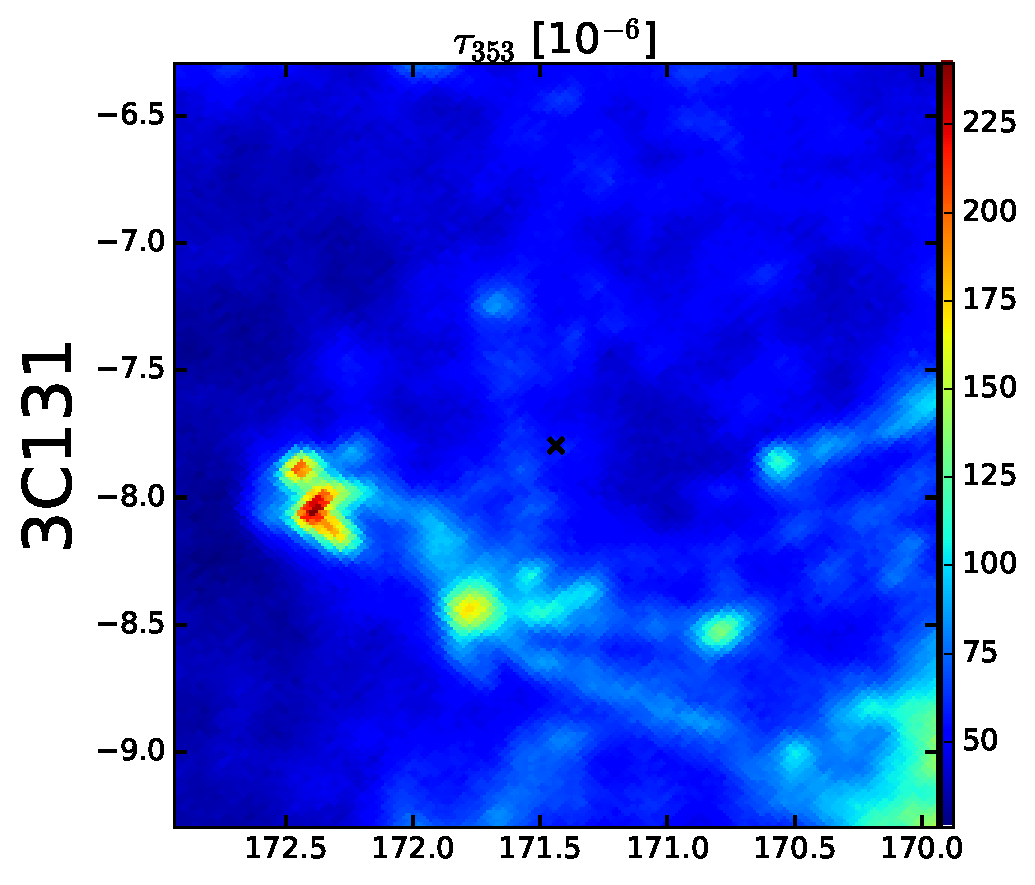
\includegraphics[scale=0.23]{fig/src_eg_apd0_r0c0.eps}
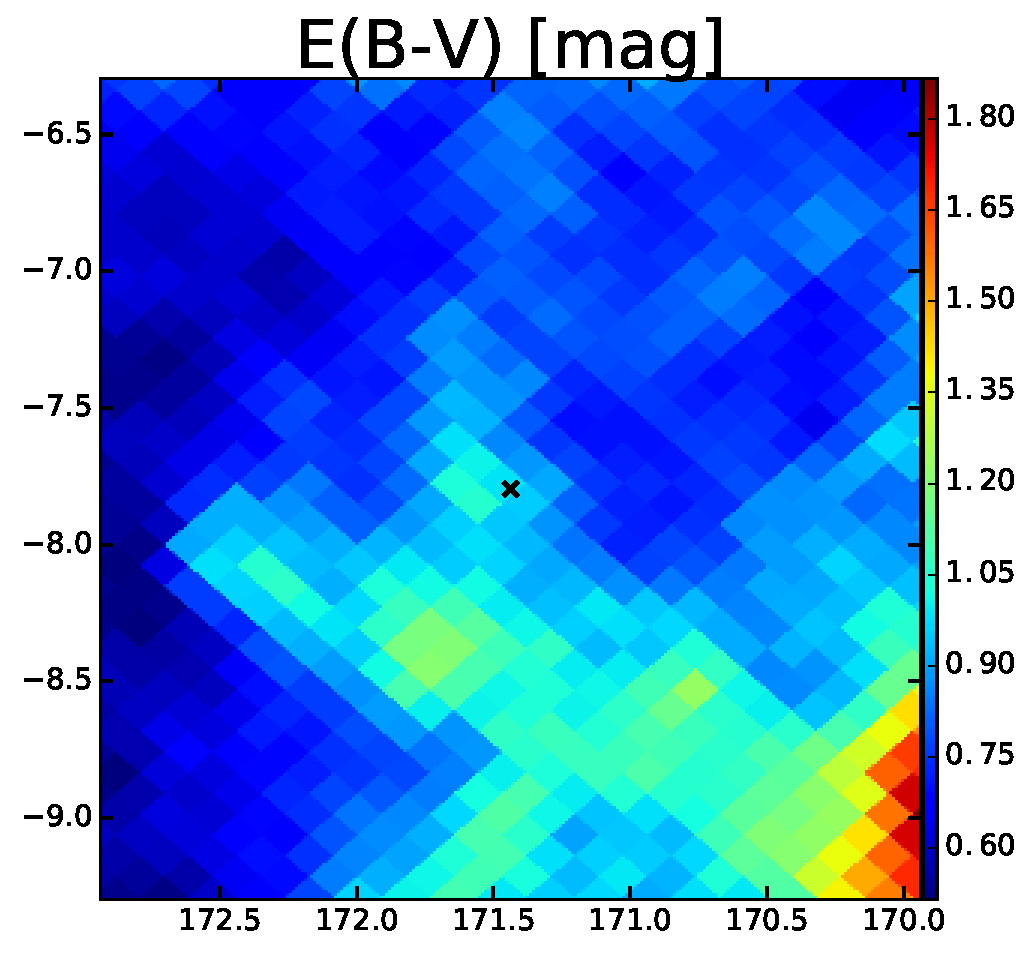
\includegraphics[scale=0.21]{fig/src_eg_apd0_r0c1.eps}
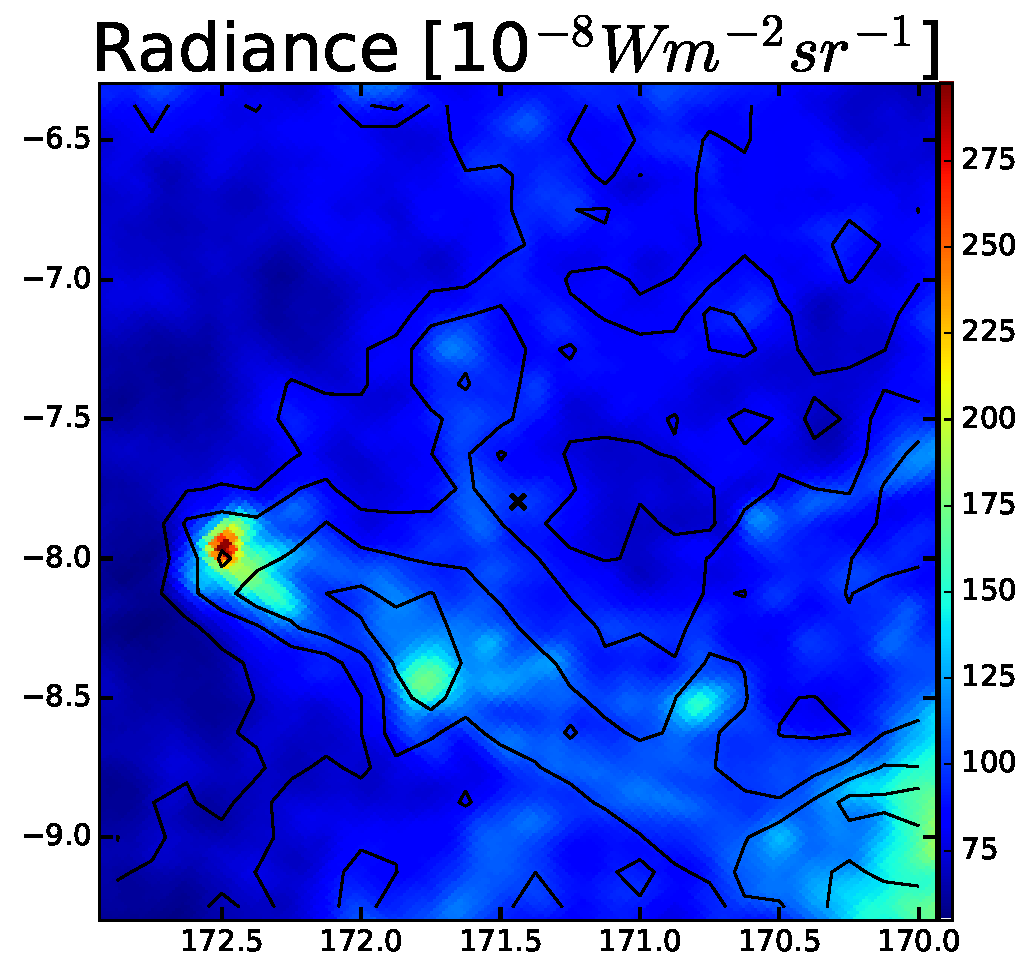
\includegraphics[scale=0.21]{fig/src_eg_apd0_r0c2.eps}
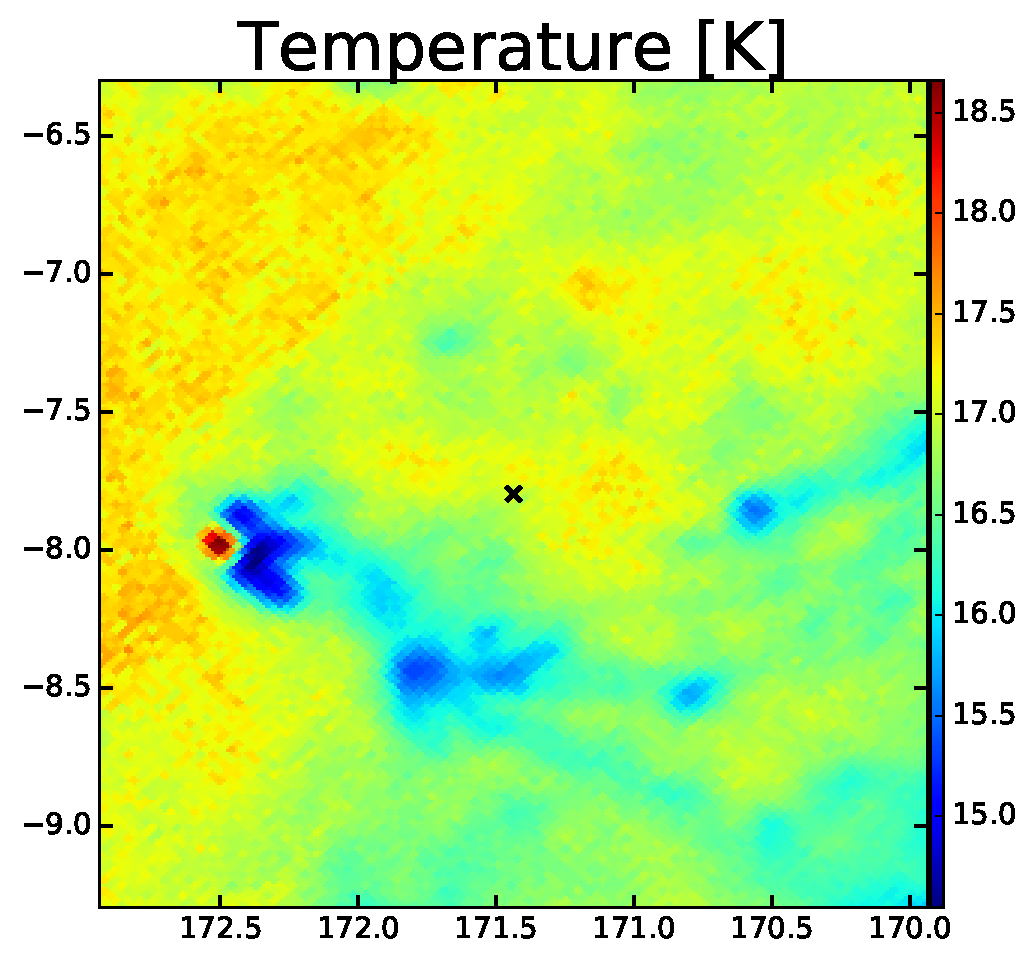
\includegraphics[scale=0.21]{fig/src_eg_apd0_r0c3.eps}
%

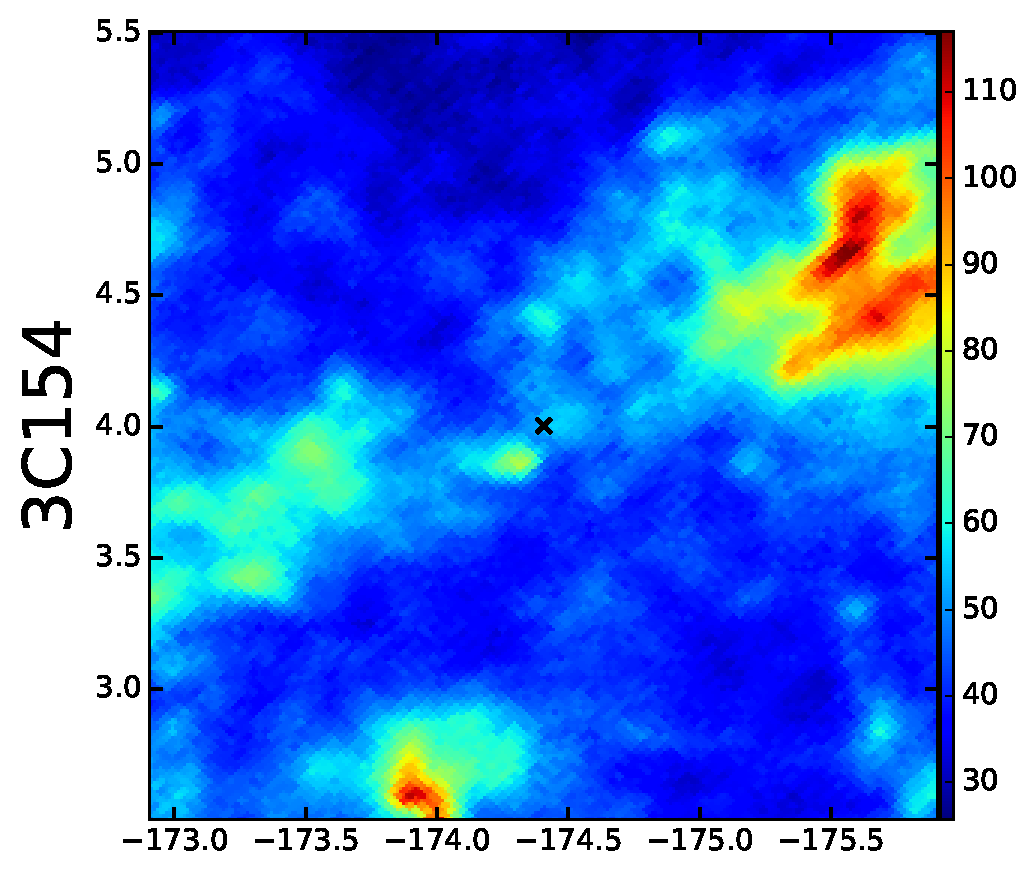
\includegraphics[scale=0.23]{fig/src_eg_apd0_r1c0.eps}
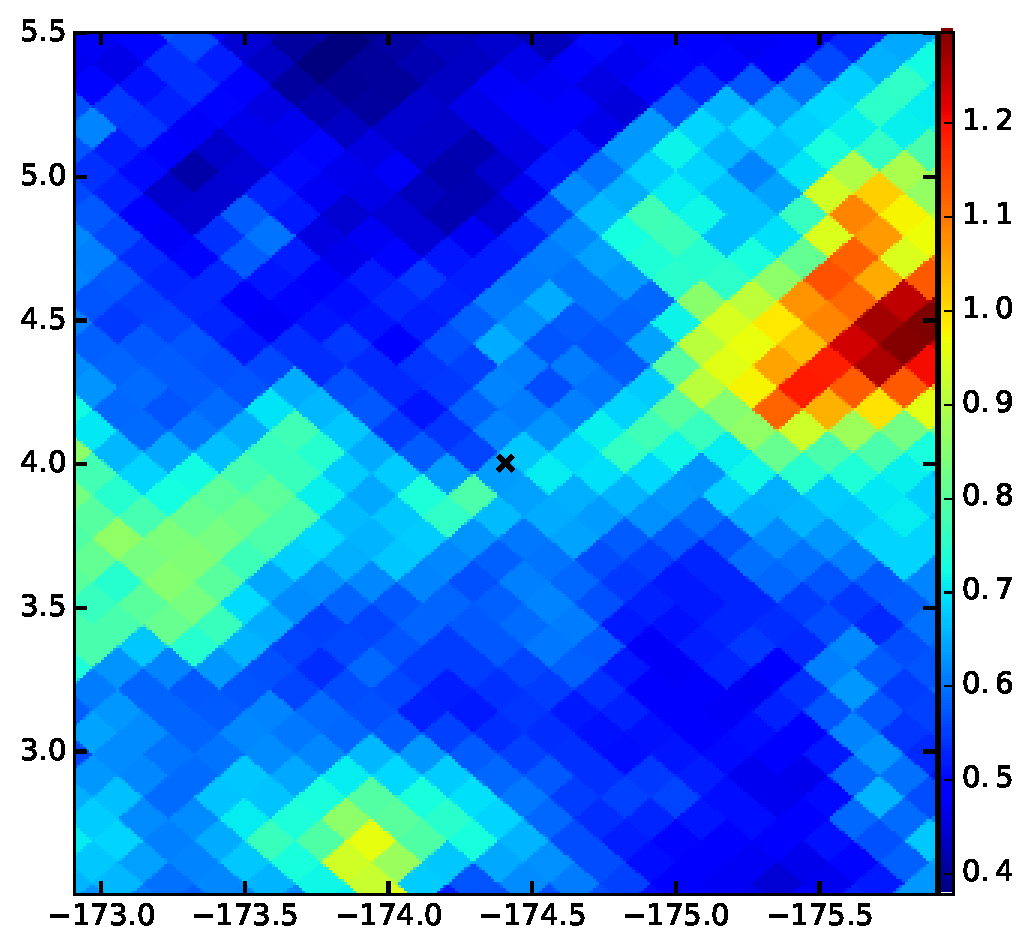
\includegraphics[scale=0.21]{fig/src_eg_apd0_r1c1.eps}
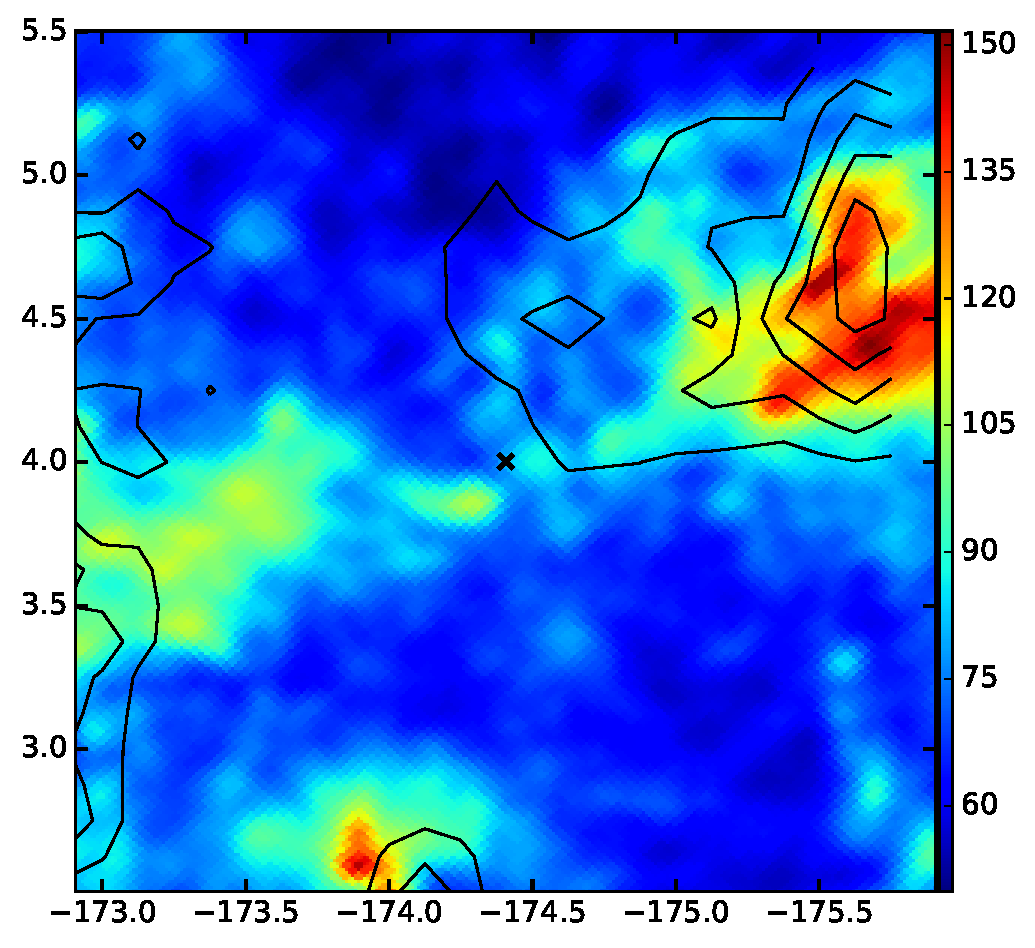
\includegraphics[scale=0.21]{fig/src_eg_apd0_r1c2.eps}
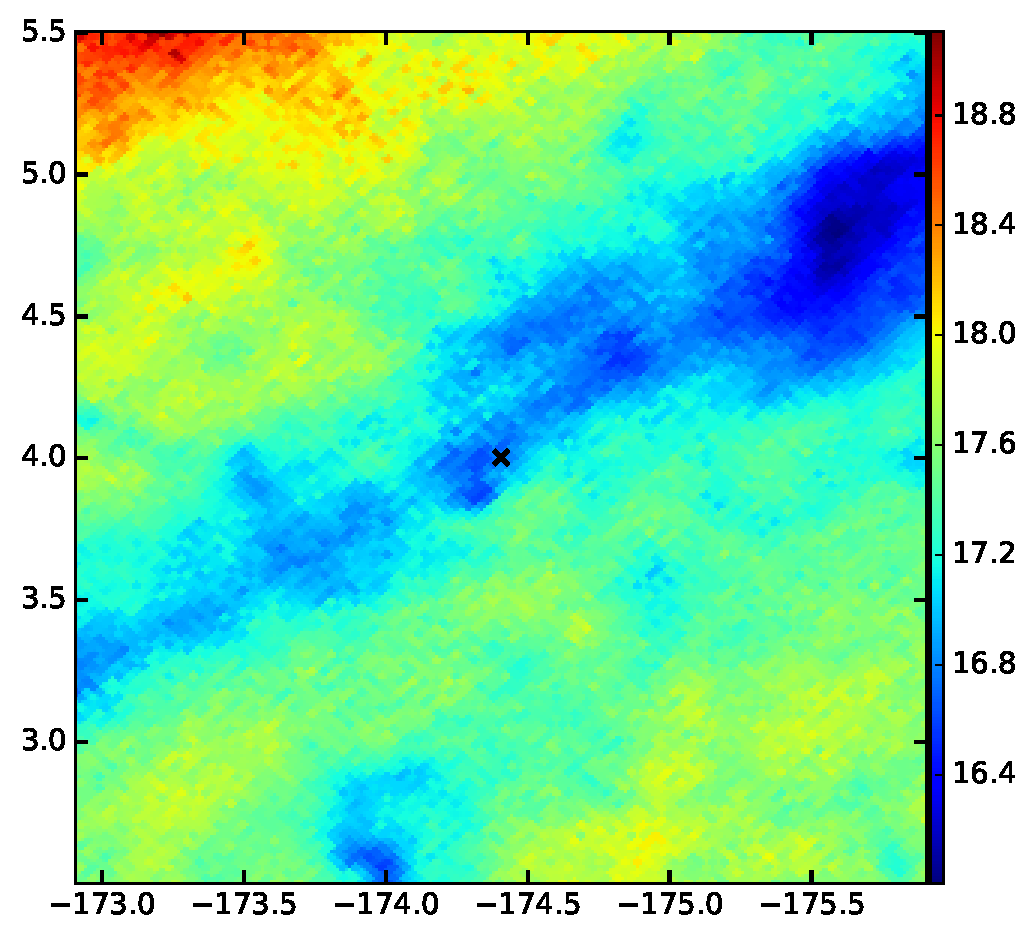
\includegraphics[scale=0.21]{fig/src_eg_apd0_r1c3.eps}
%

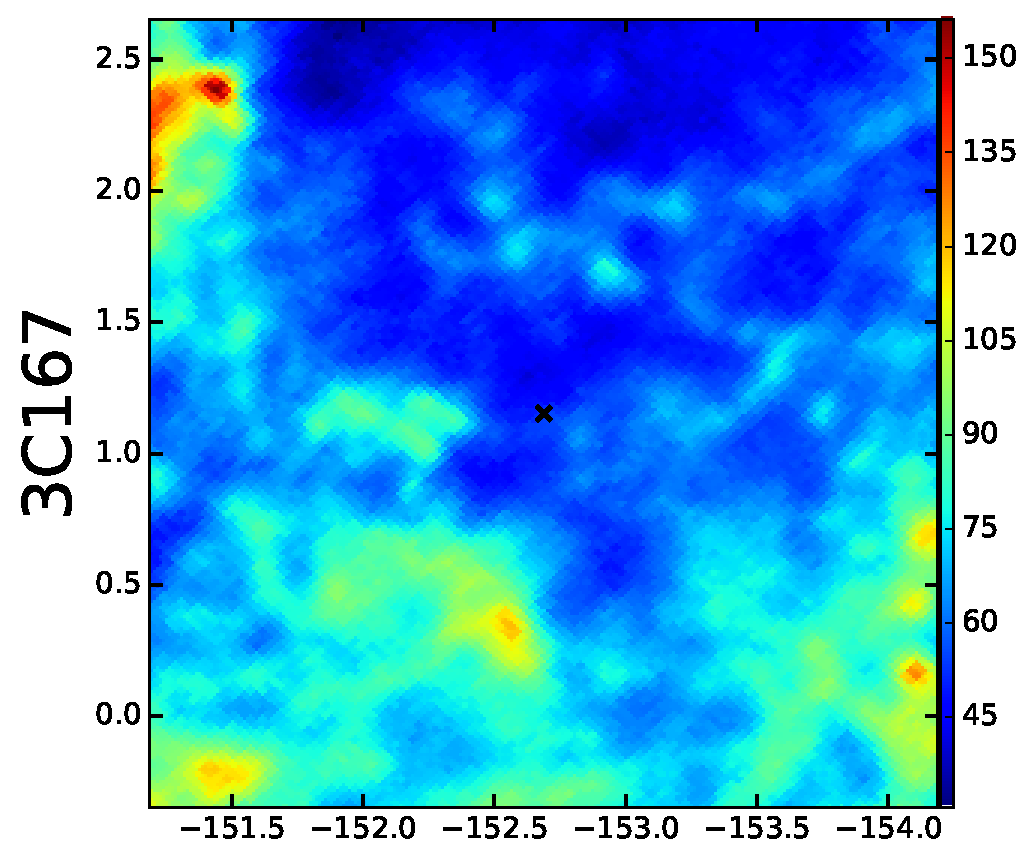
\includegraphics[scale=0.23]{fig/src_eg_apd0_r2c0.eps}
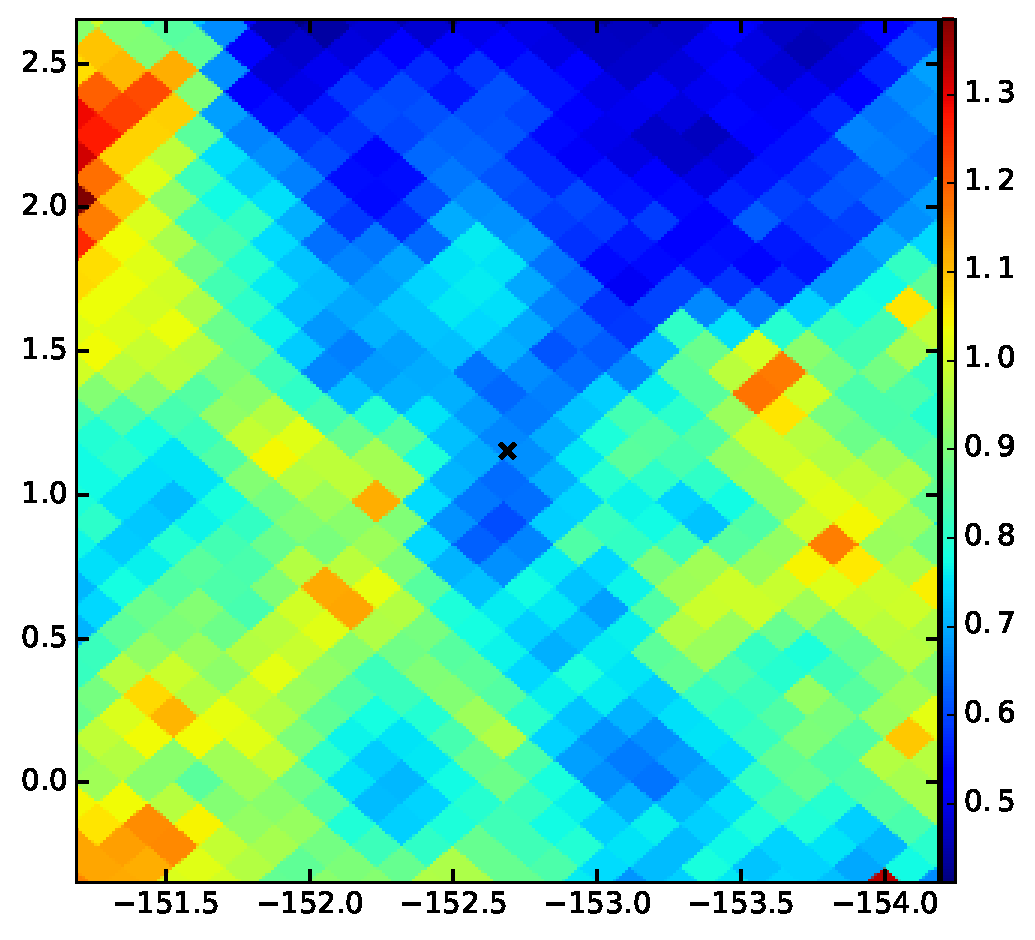
\includegraphics[scale=0.21]{fig/src_eg_apd0_r2c1.eps}
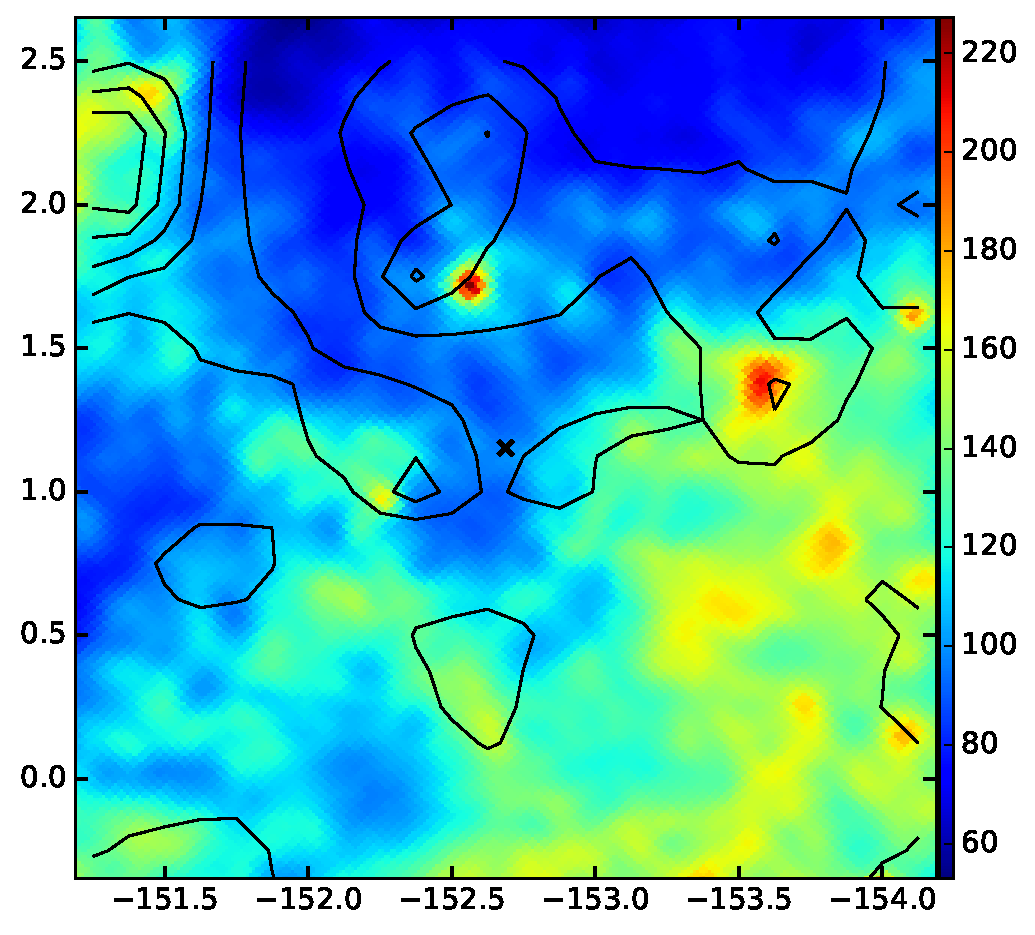
\includegraphics[scale=0.21]{fig/src_eg_apd0_r2c2.eps}
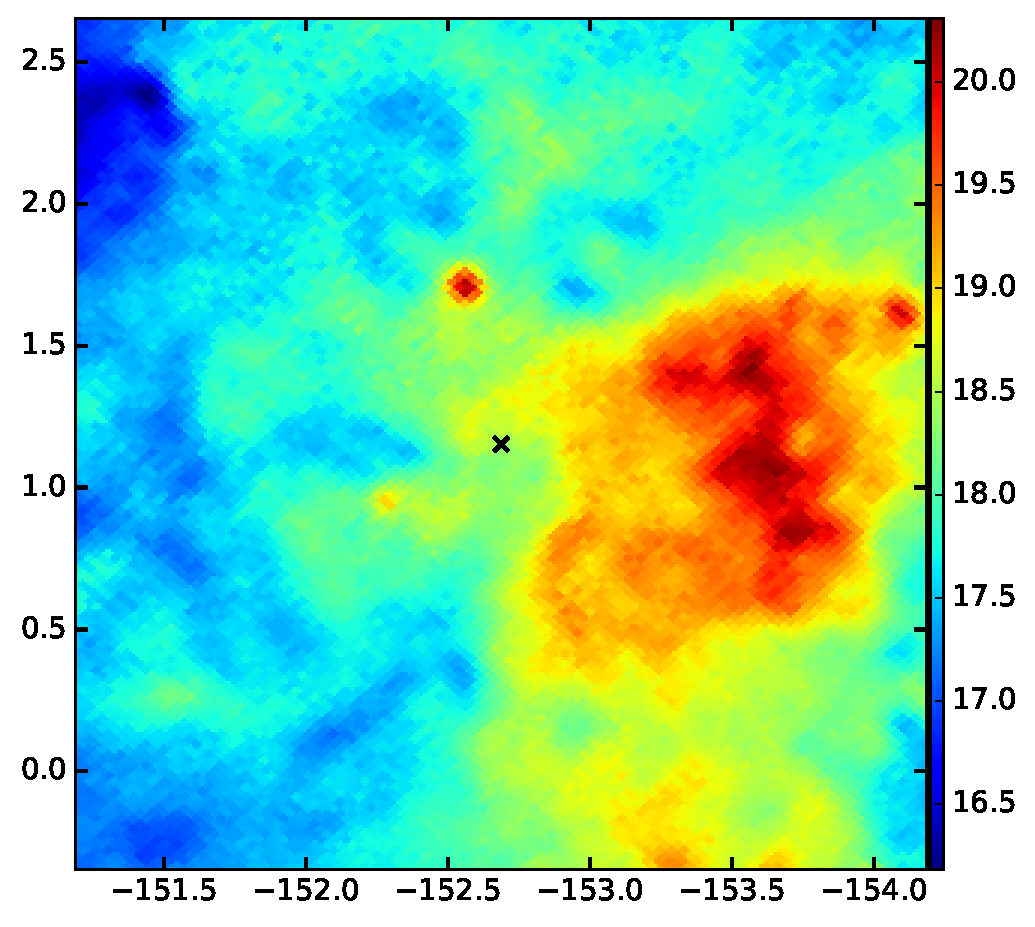
\includegraphics[scale=0.21]{fig/src_eg_apd0_r2c3.eps}
%
\caption{Examples of 3 sighlines towards radio sources in 4 different dust maps (3$\times$3 degrees in Galactic coordinates) adopted from Planck collaboration 2014 ($\tau_{353}$, radiance and temperature, Nside = 1024) and Schlafly et. al. 2011 (E(B-V), Nside = 512). The 'X' markers at centers show the locations of the sources. The contours represent the W$_{CO(1-0)}$ from Dame et al. 2001.}
\label{fig:apd0}
\end{figure*}

\begin{figure*}
\centering     
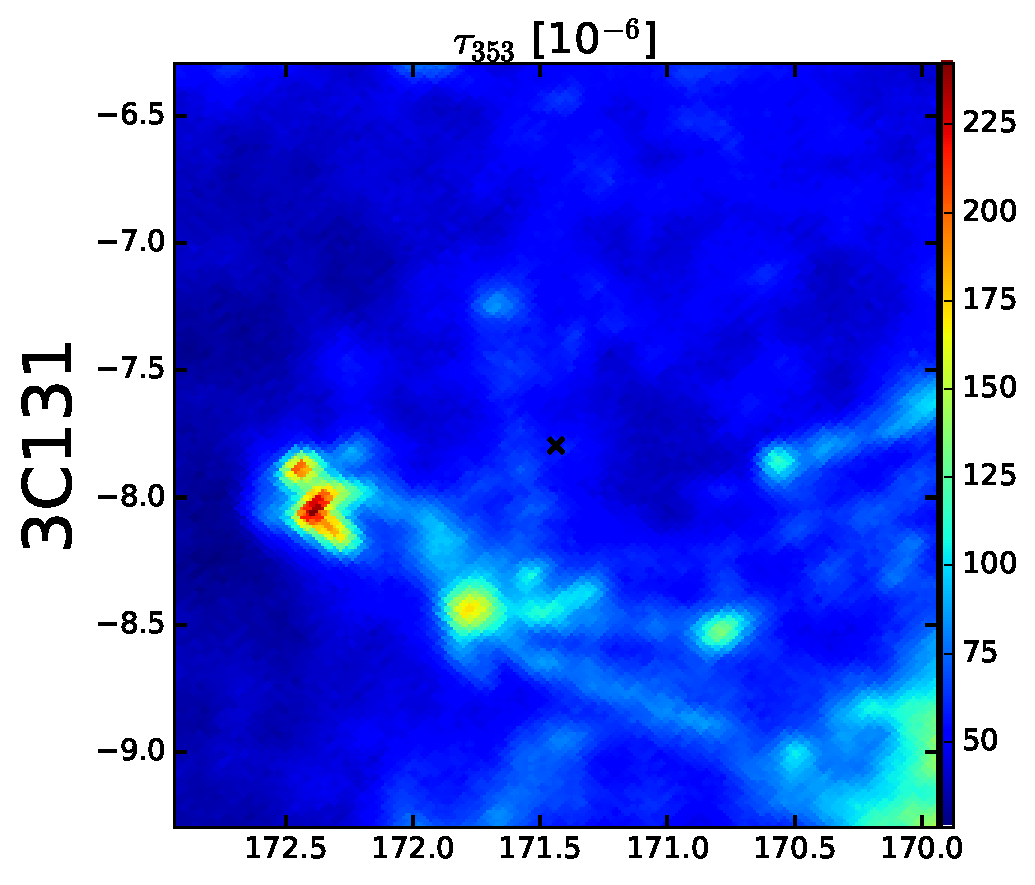
\includegraphics[scale=0.23]{fig/src_eg_apd0_r0c0.eps}
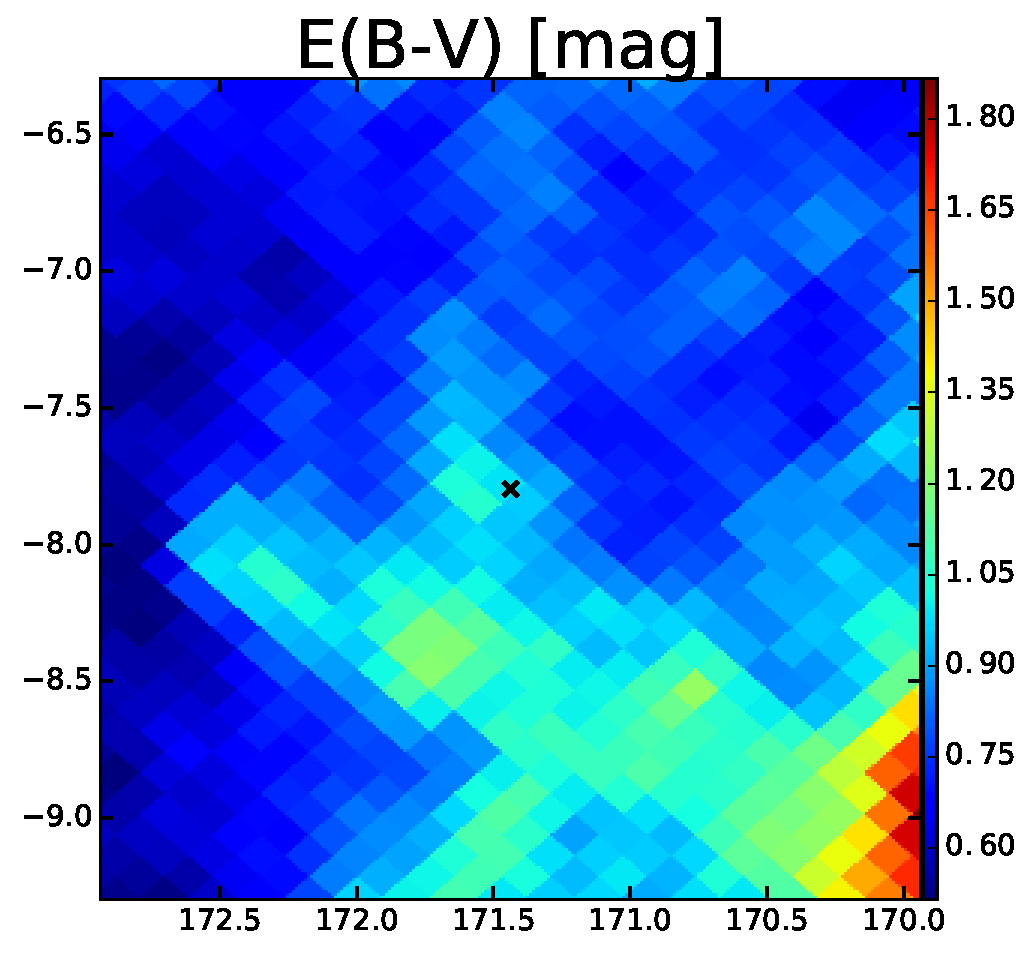
\includegraphics[scale=0.21]{fig/src_eg_apd0_r0c1.eps}
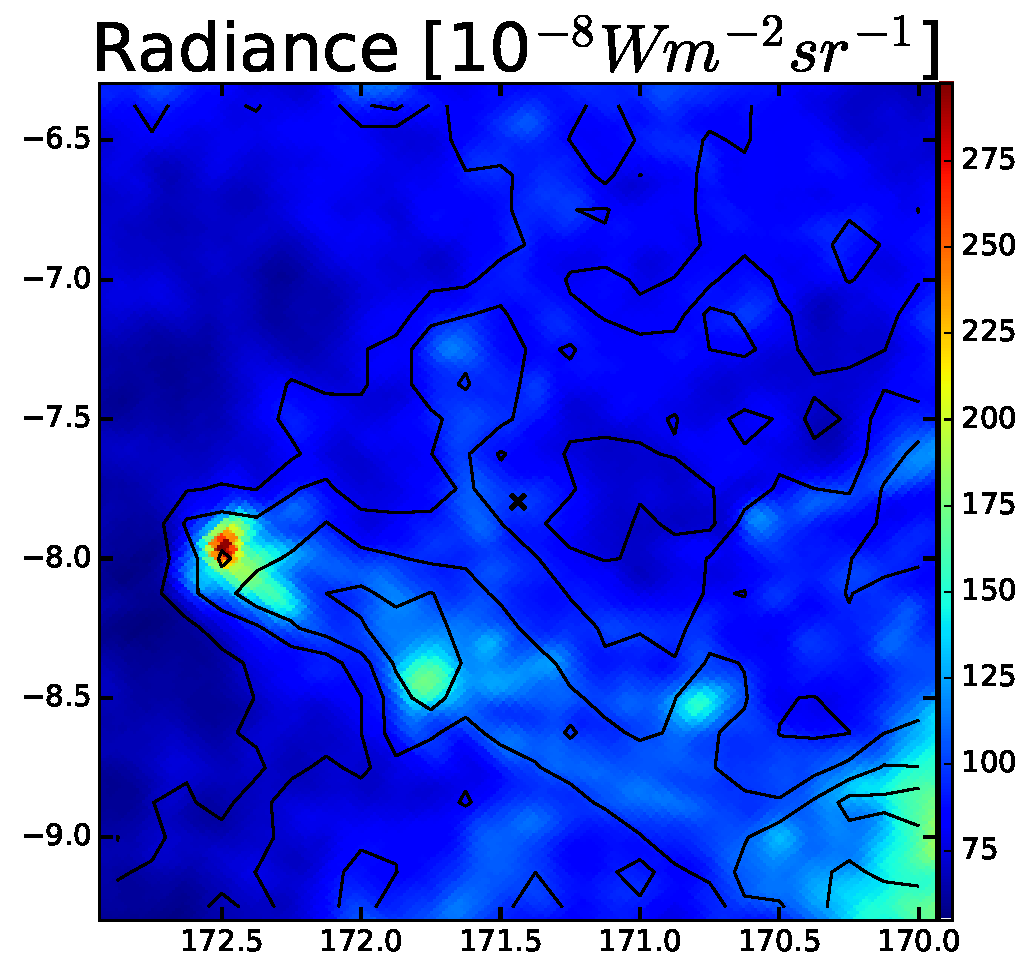
\includegraphics[scale=0.21]{fig/src_eg_apd0_r0c2.eps}
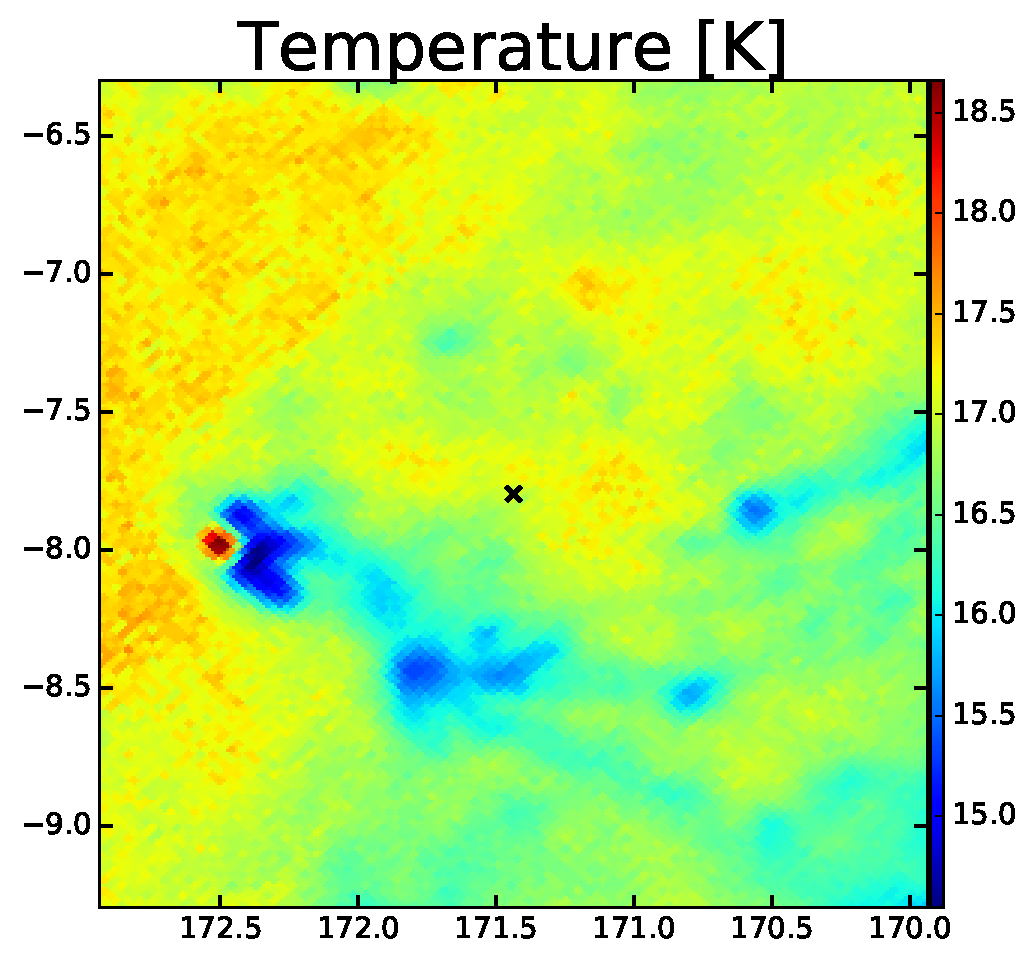
\includegraphics[scale=0.21]{fig/src_eg_apd0_r0c3.eps}
%

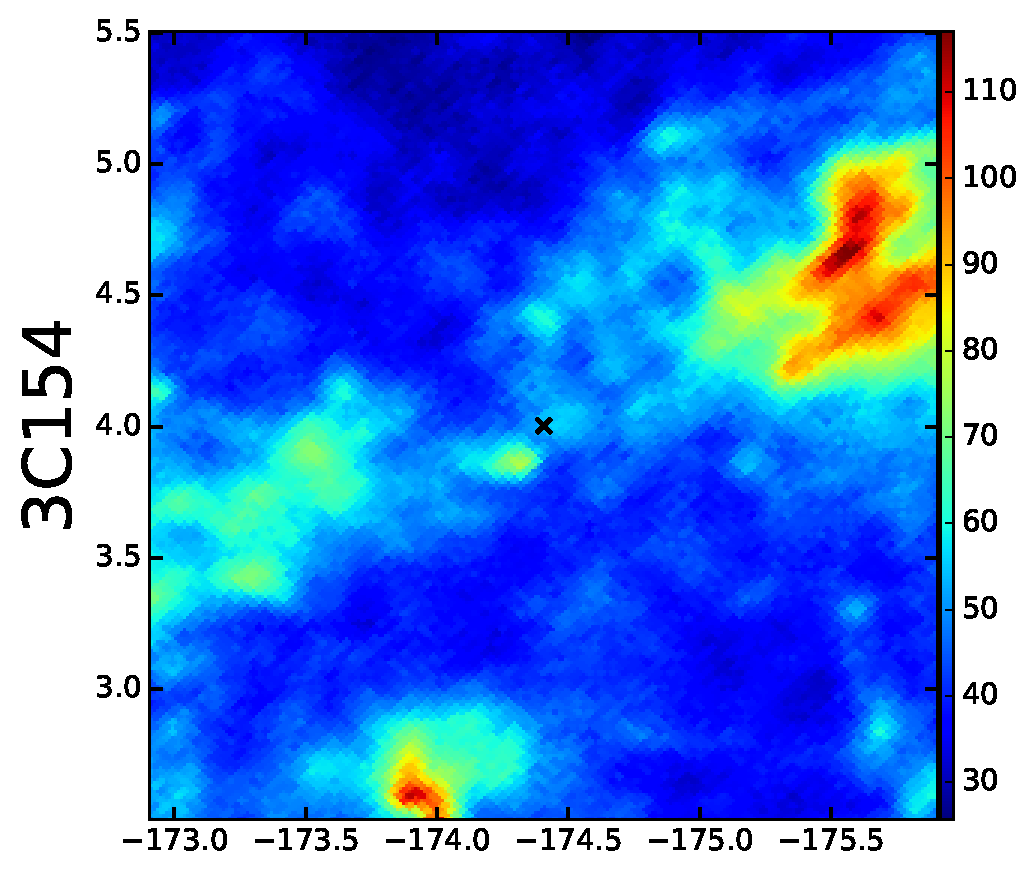
\includegraphics[scale=0.23]{fig/src_eg_apd0_r1c0.eps}
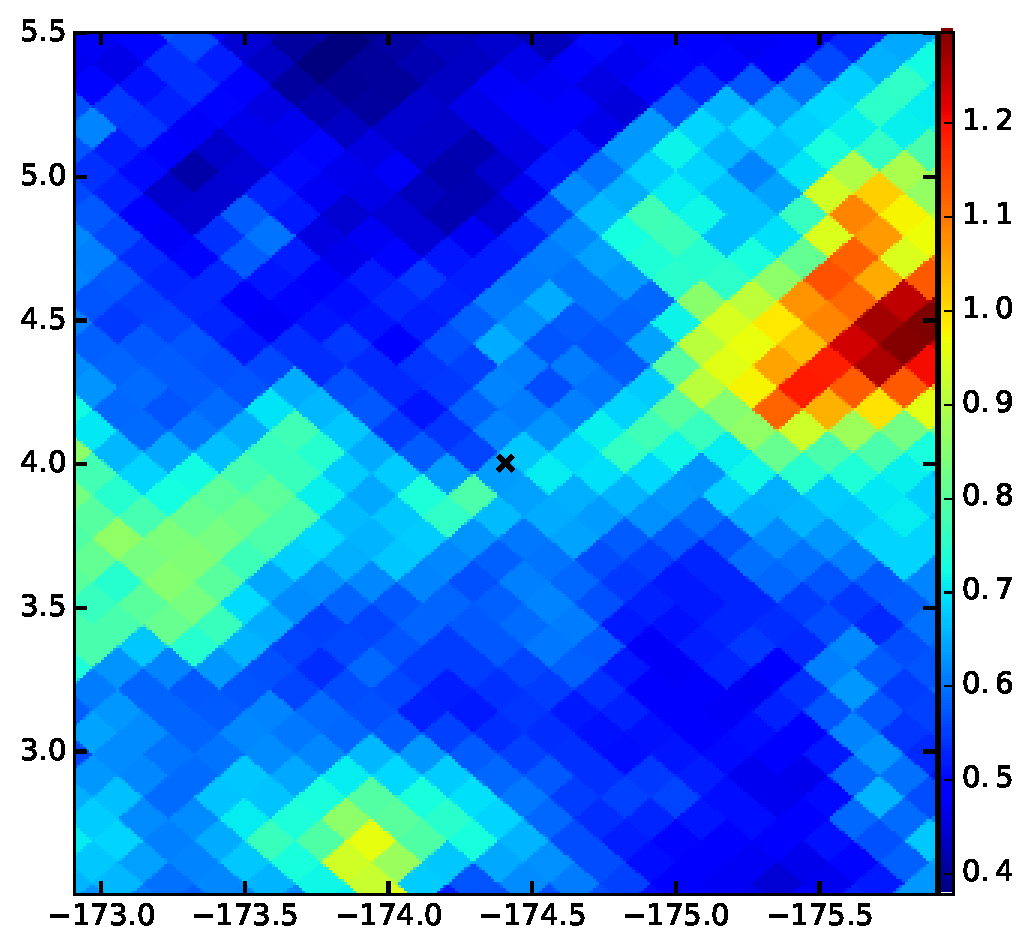
\includegraphics[scale=0.21]{fig/src_eg_apd0_r1c1.eps}
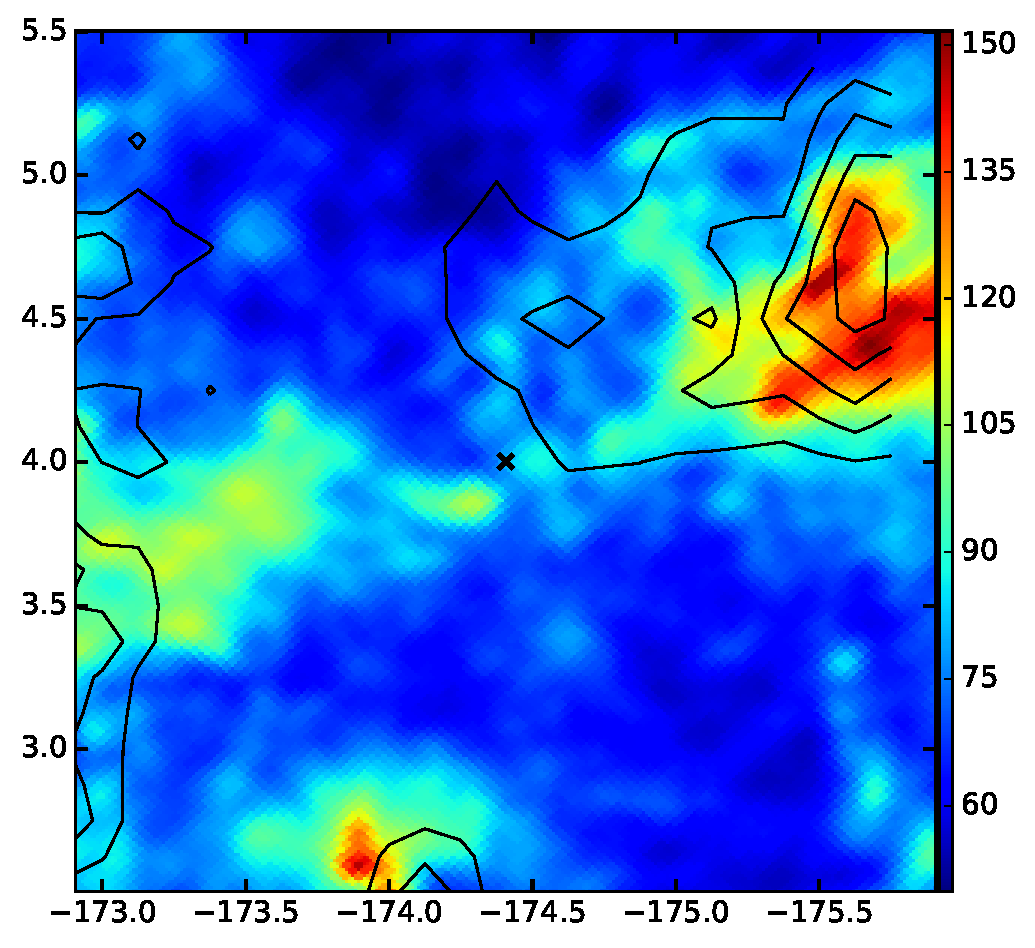
\includegraphics[scale=0.21]{fig/src_eg_apd0_r1c2.eps}
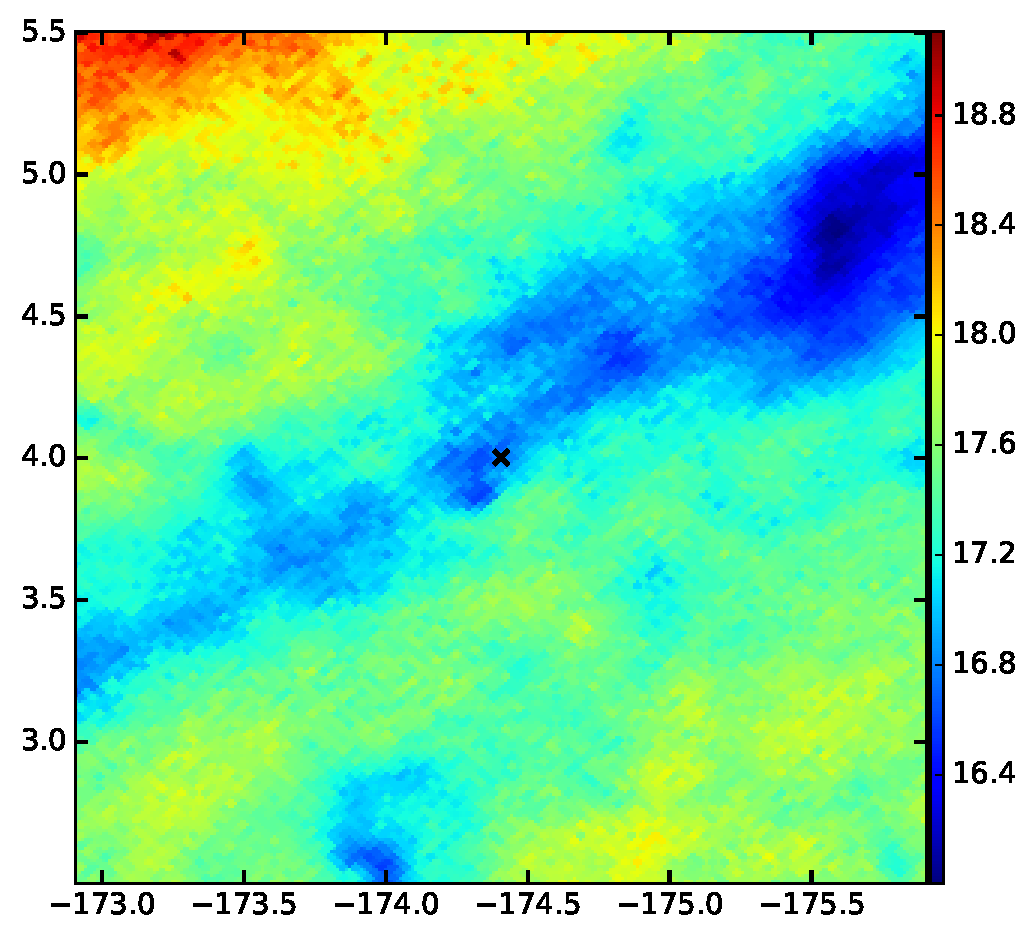
\includegraphics[scale=0.21]{fig/src_eg_apd0_r1c3.eps}
%

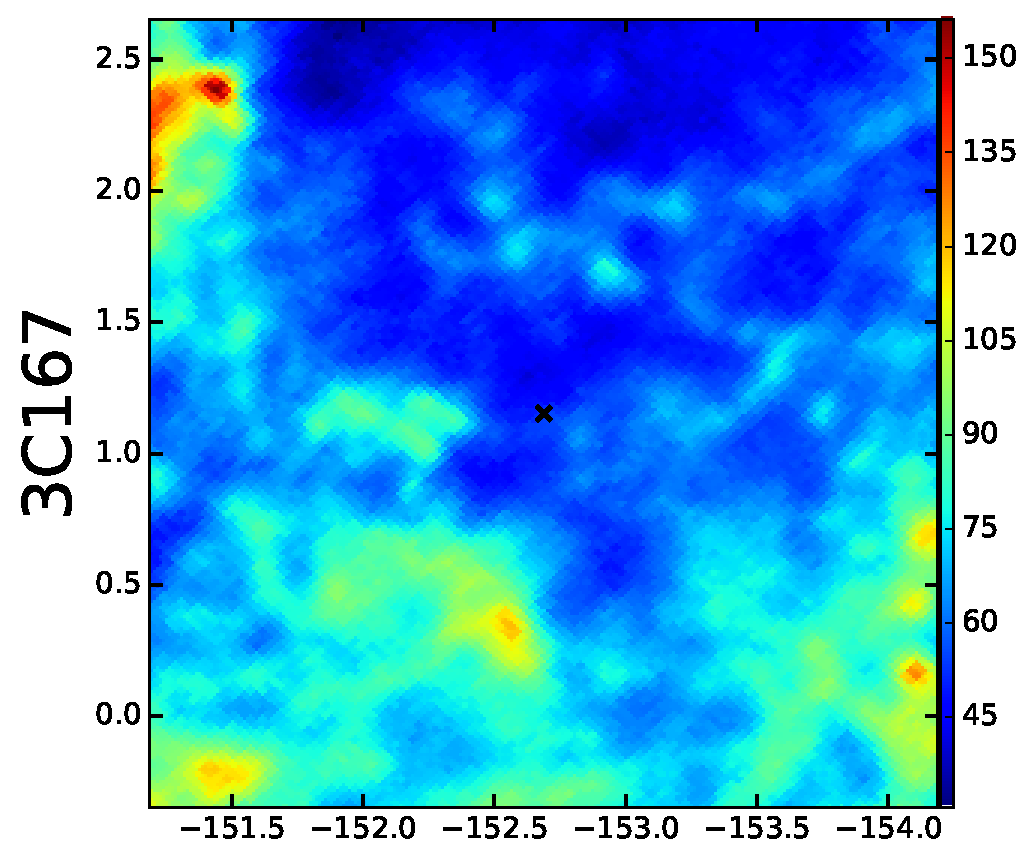
\includegraphics[scale=0.23]{fig/src_eg_apd0_r2c0.eps}
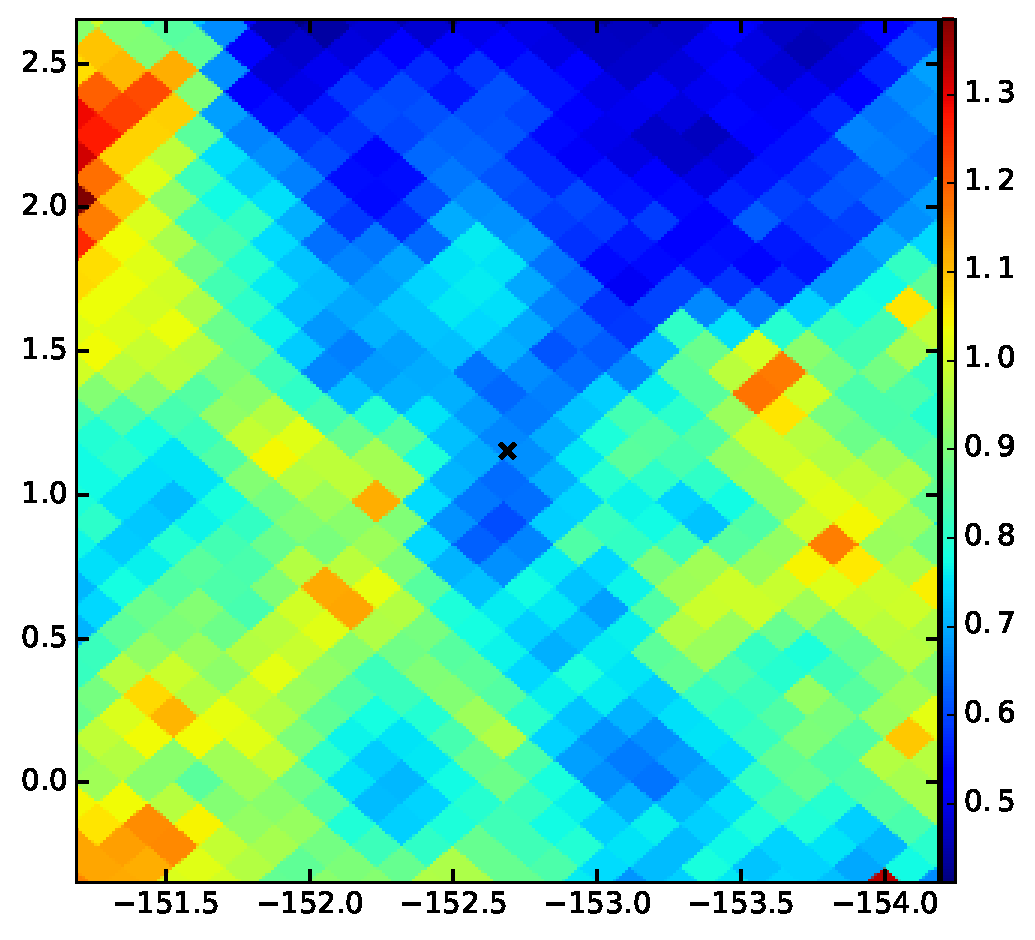
\includegraphics[scale=0.21]{fig/src_eg_apd0_r2c1.eps}
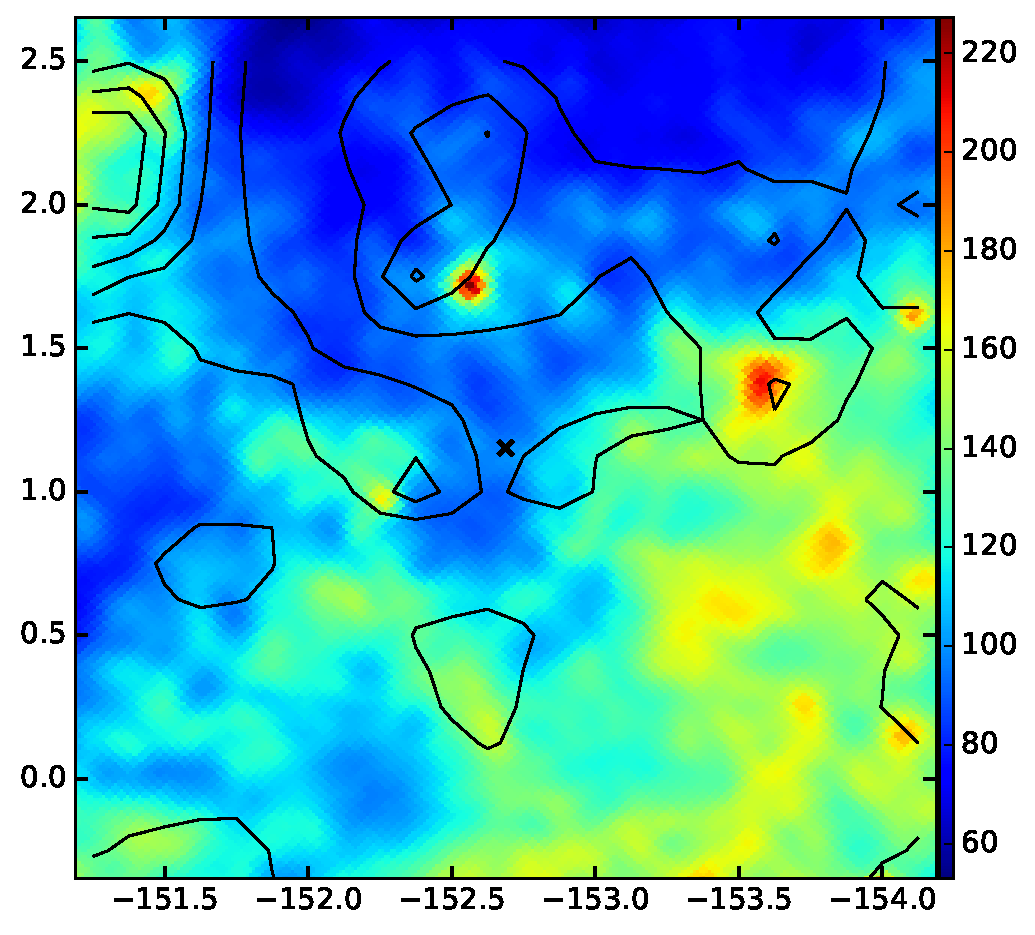
\includegraphics[scale=0.21]{fig/src_eg_apd0_r2c2.eps}
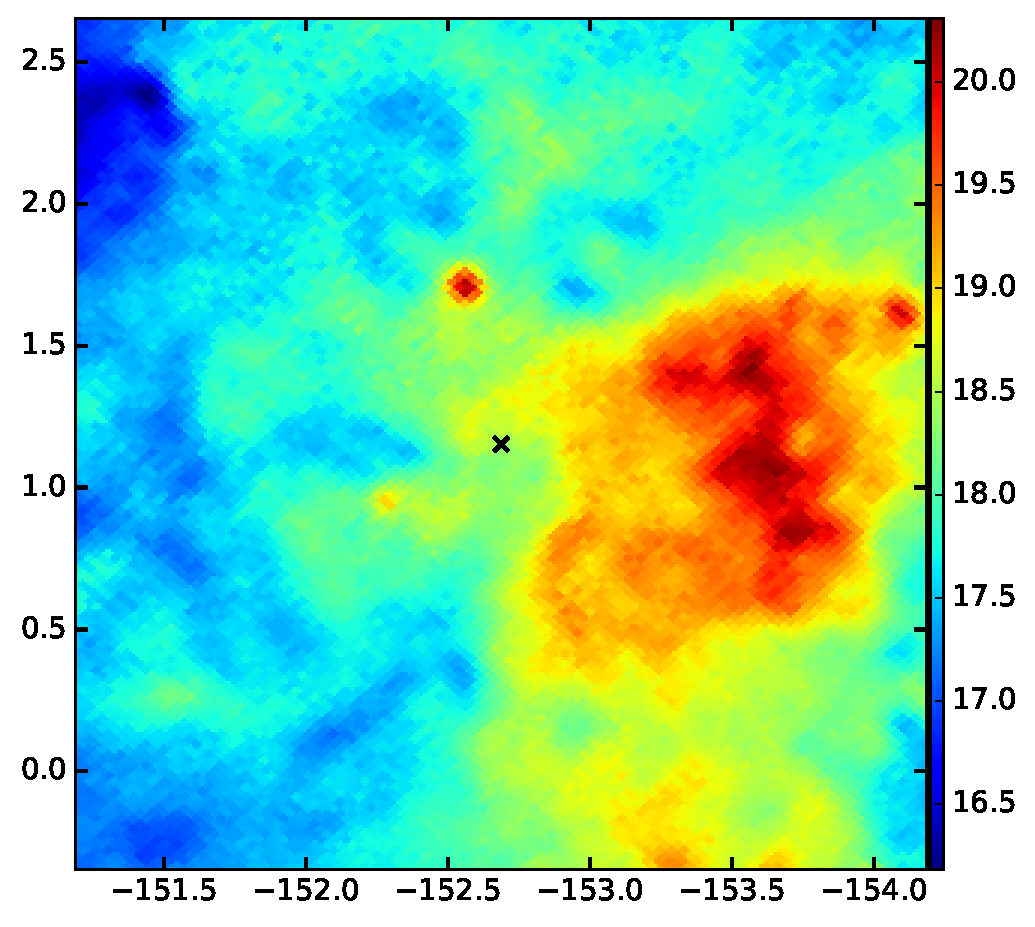
\includegraphics[scale=0.21]{fig/src_eg_apd0_r2c3.eps}
%
\caption{See Figure \ref{fig:apd0} for details.}
\label{fig:apd1}
\end{figure*}


\begin{figure*}
\centering     
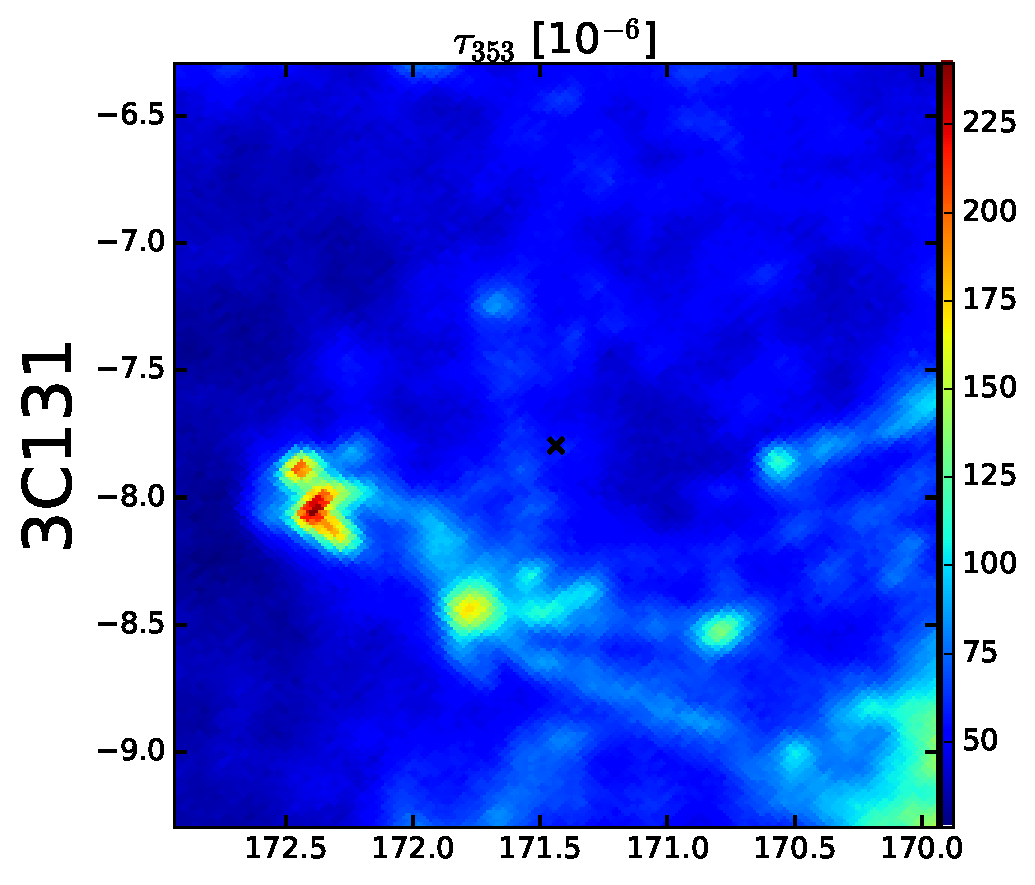
\includegraphics[scale=0.23]{fig/src_eg_apd0_r0c0.eps}
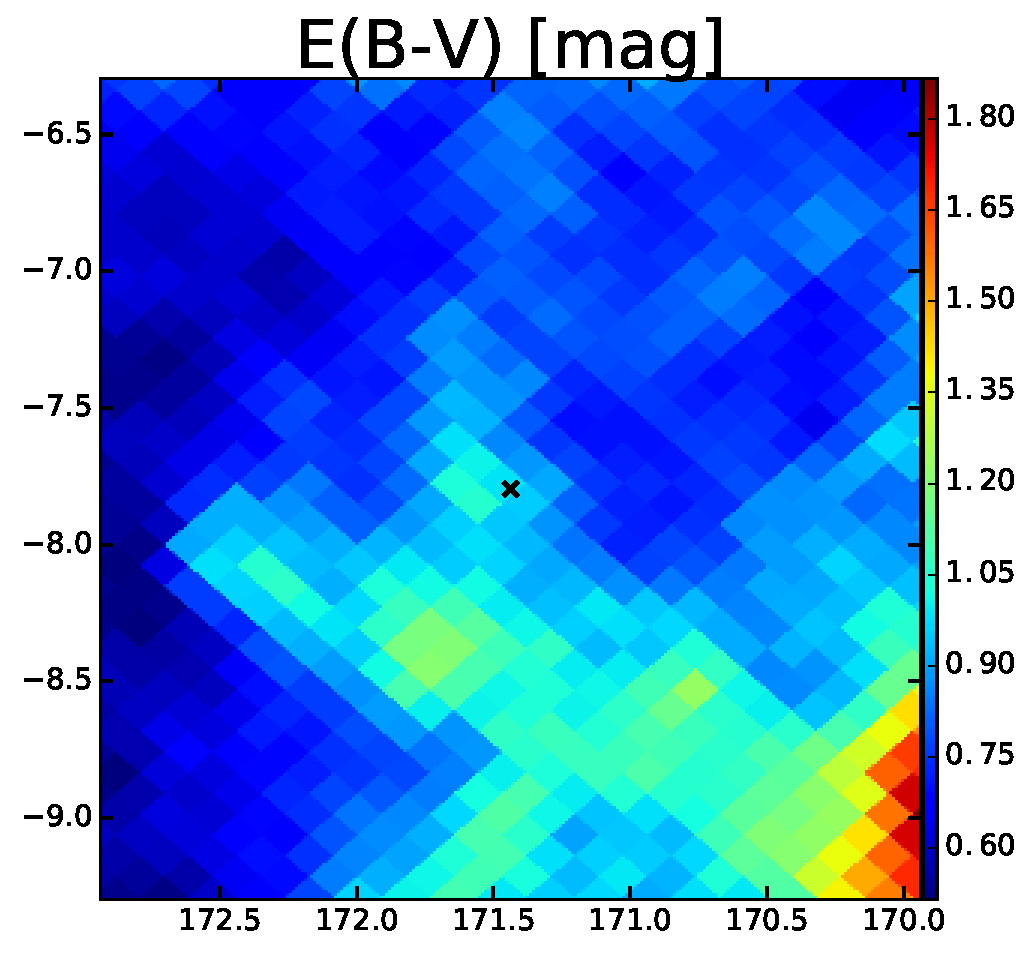
\includegraphics[scale=0.21]{fig/src_eg_apd0_r0c1.eps}
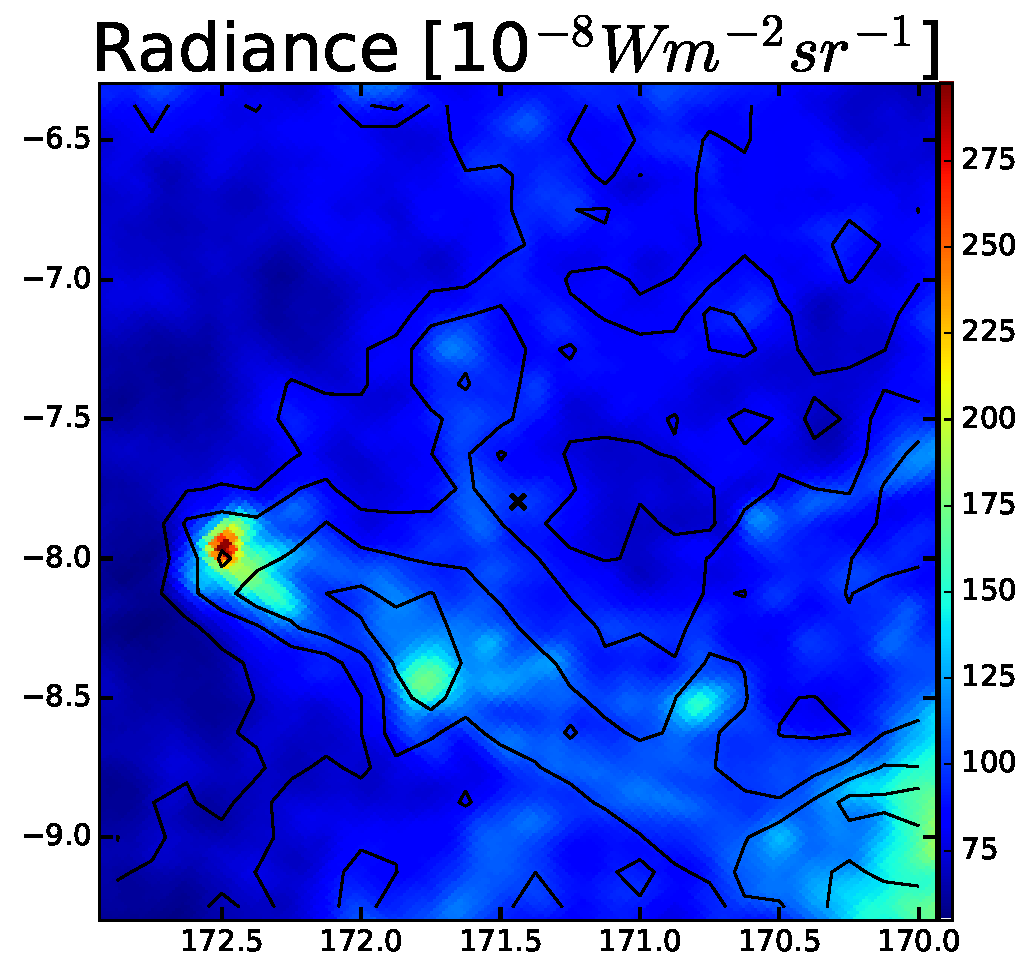
\includegraphics[scale=0.21]{fig/src_eg_apd0_r0c2.eps}
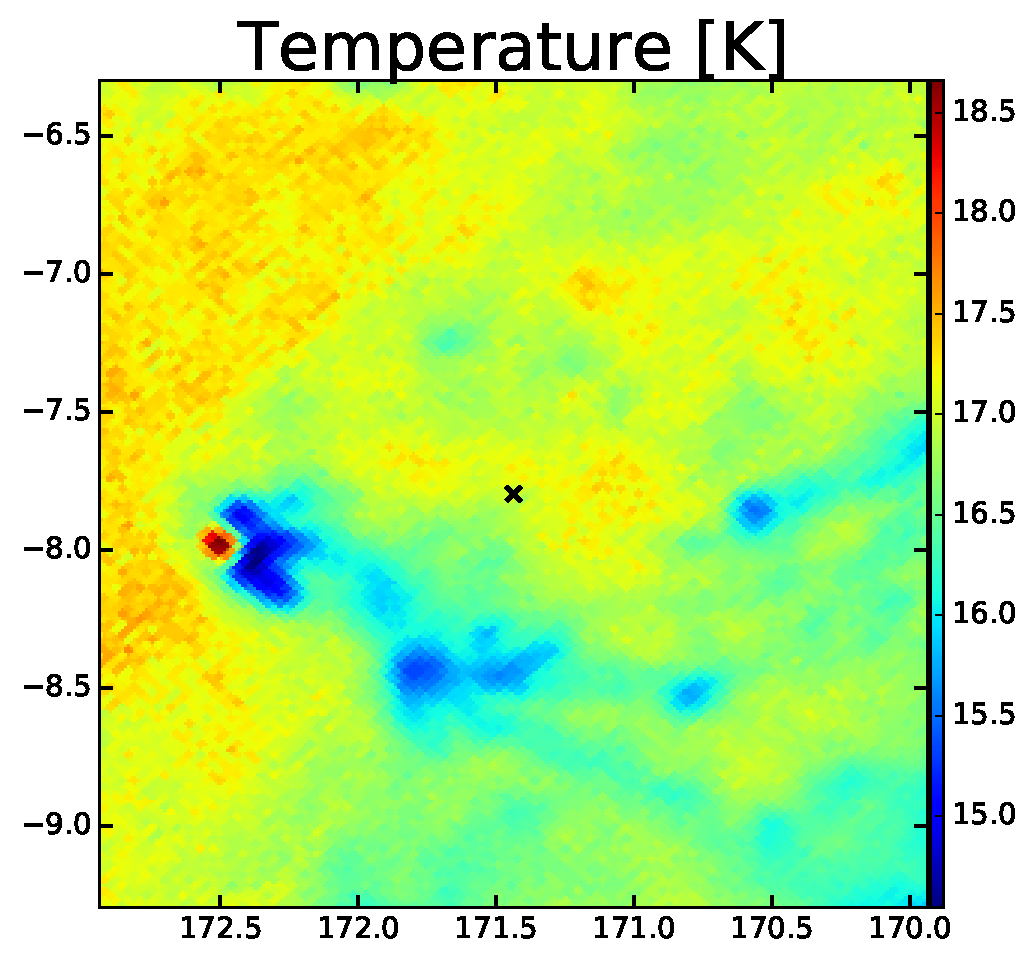
\includegraphics[scale=0.21]{fig/src_eg_apd0_r0c3.eps}
%

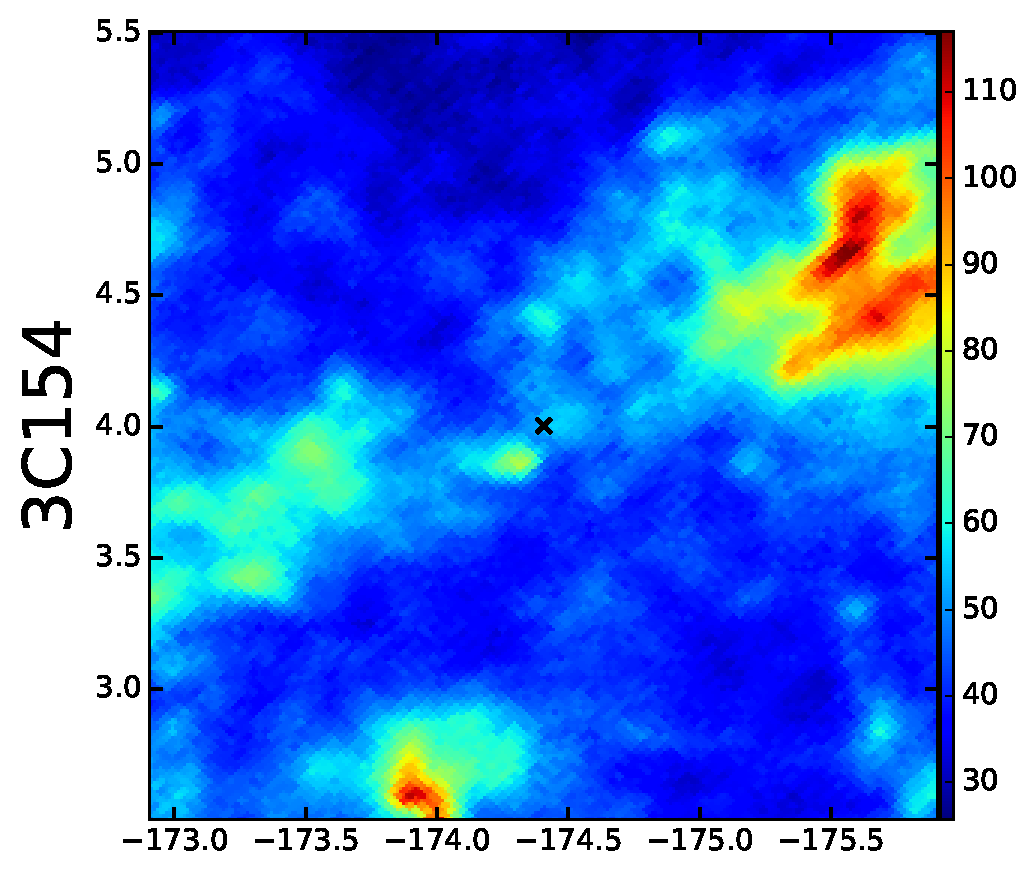
\includegraphics[scale=0.23]{fig/src_eg_apd0_r1c0.eps}
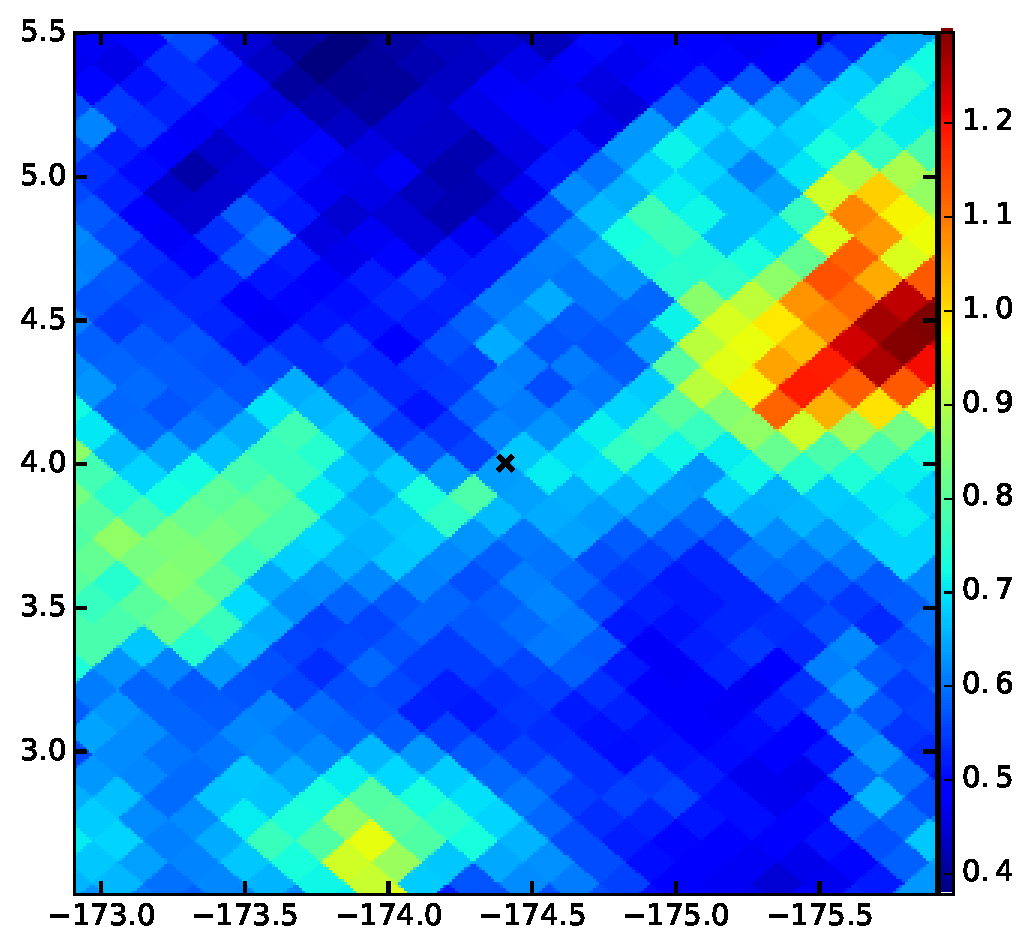
\includegraphics[scale=0.21]{fig/src_eg_apd0_r1c1.eps}
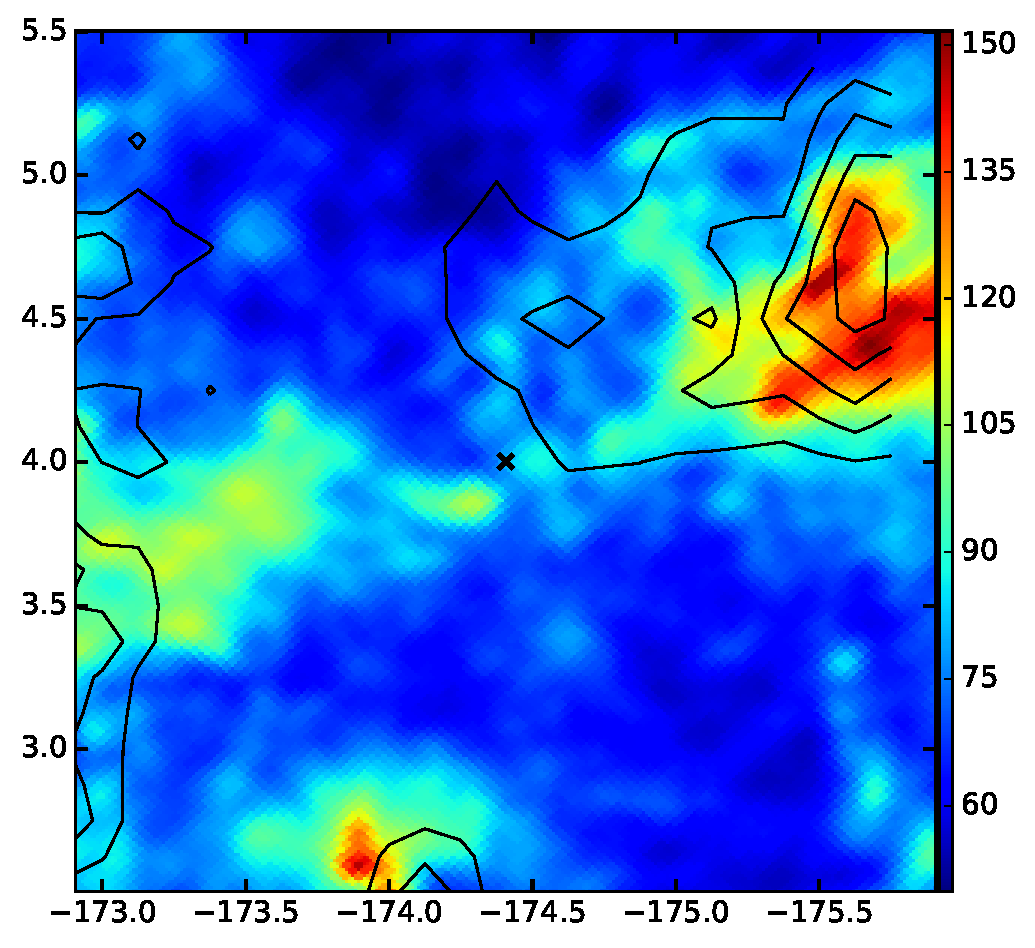
\includegraphics[scale=0.21]{fig/src_eg_apd0_r1c2.eps}
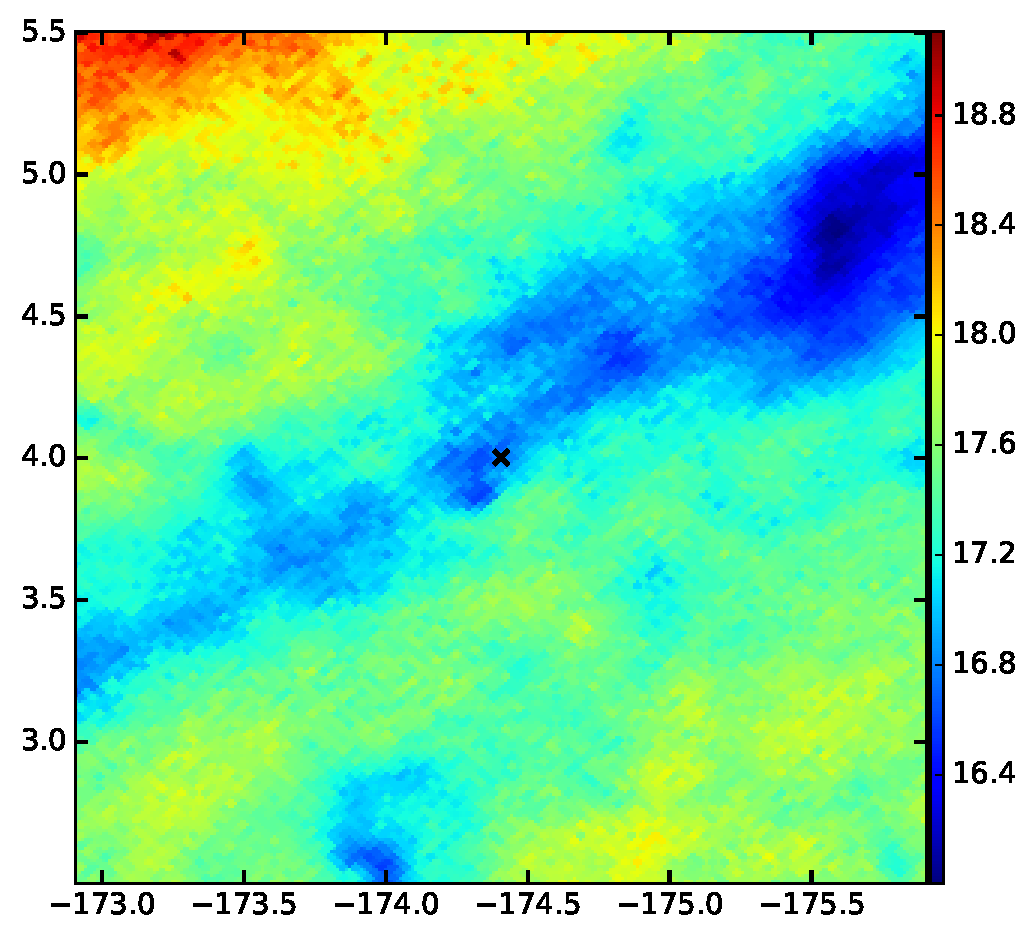
\includegraphics[scale=0.21]{fig/src_eg_apd0_r1c3.eps}
%

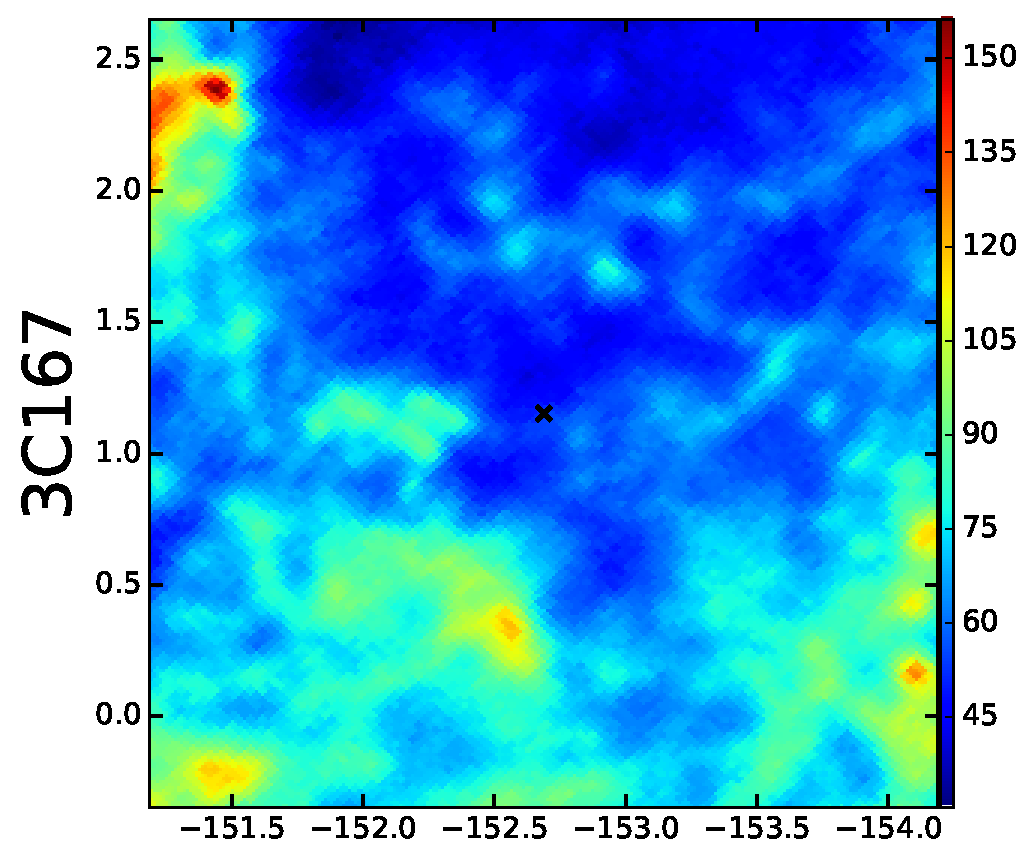
\includegraphics[scale=0.23]{fig/src_eg_apd0_r2c0.eps}
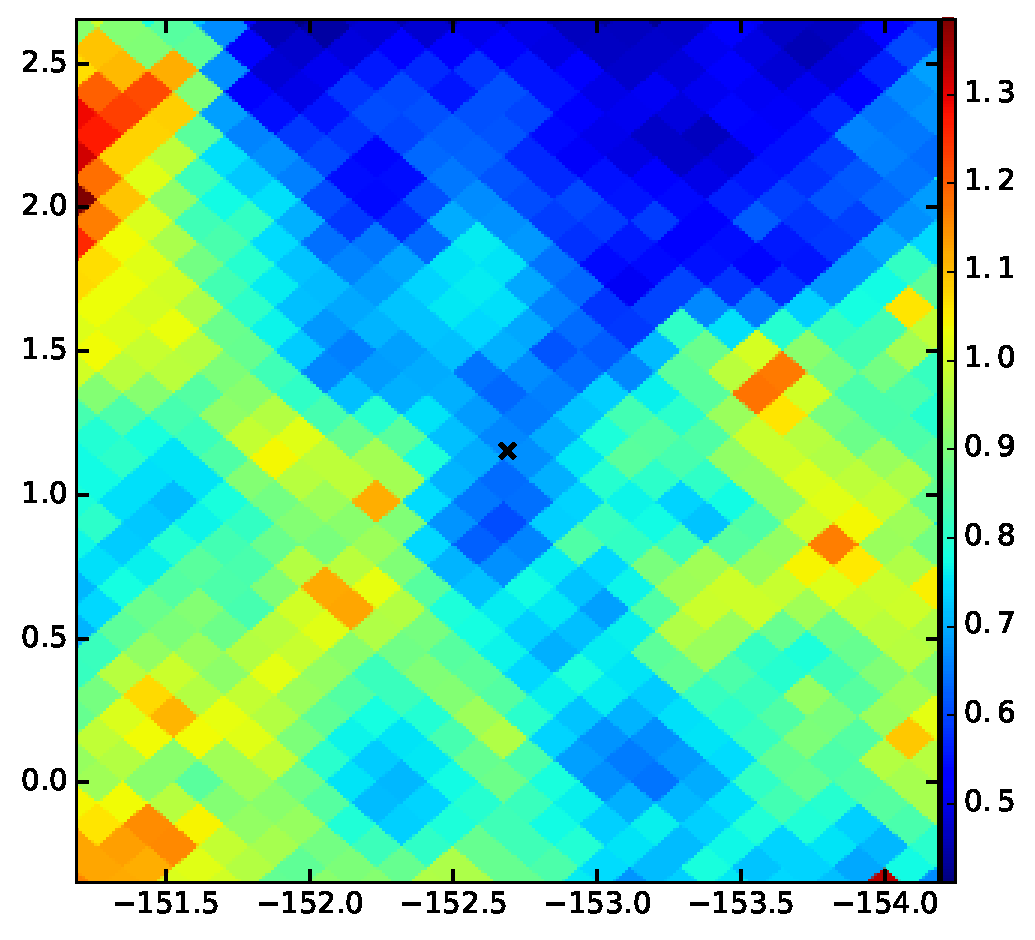
\includegraphics[scale=0.21]{fig/src_eg_apd0_r2c1.eps}
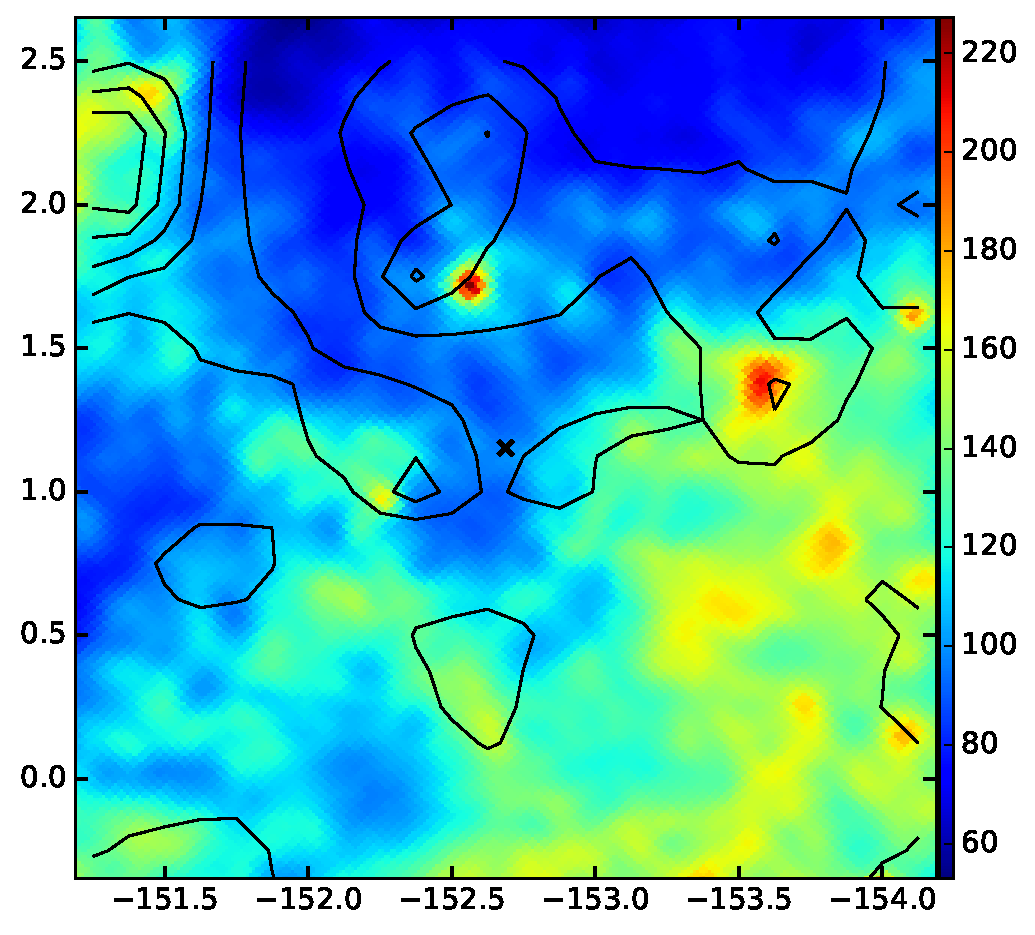
\includegraphics[scale=0.21]{fig/src_eg_apd0_r2c2.eps}
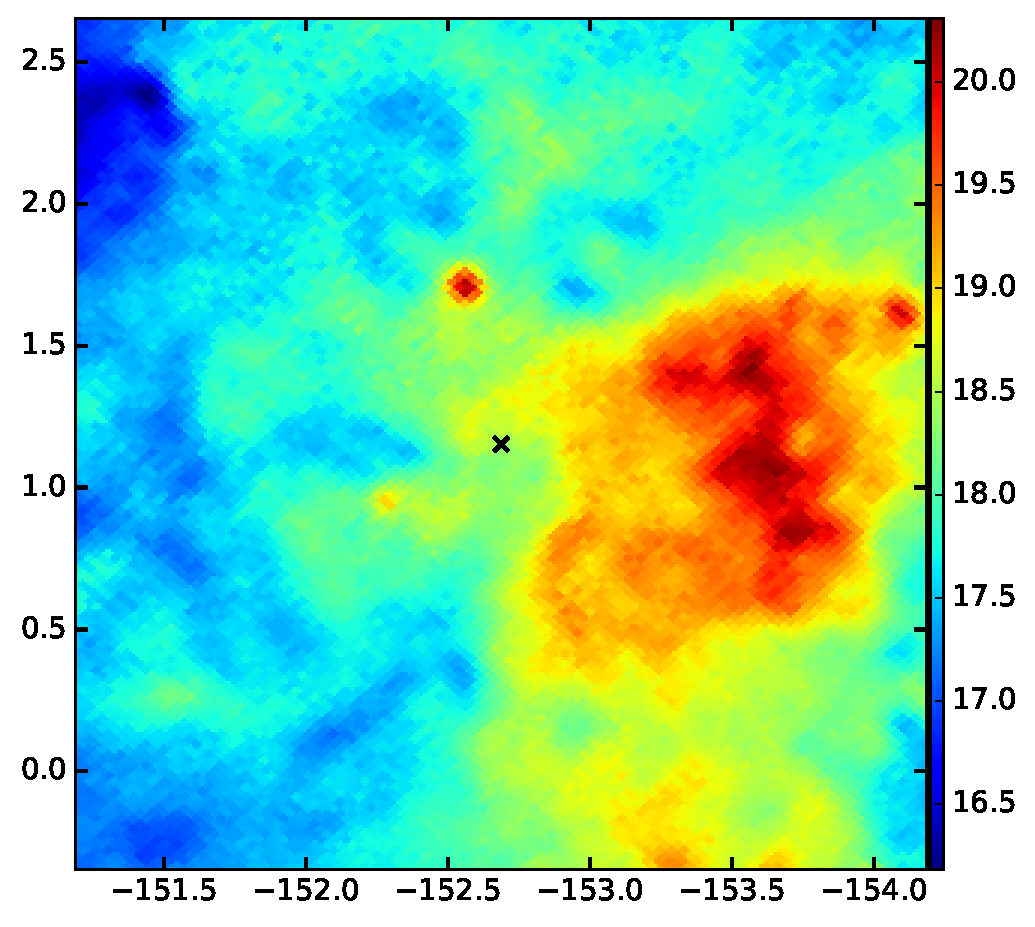
\includegraphics[scale=0.21]{fig/src_eg_apd0_r2c3.eps}
%
\caption{See Figure \ref{fig:apd0} for details.}
\label{fig:apd2}
\end{figure*}

\begin{figure*}
\centering     
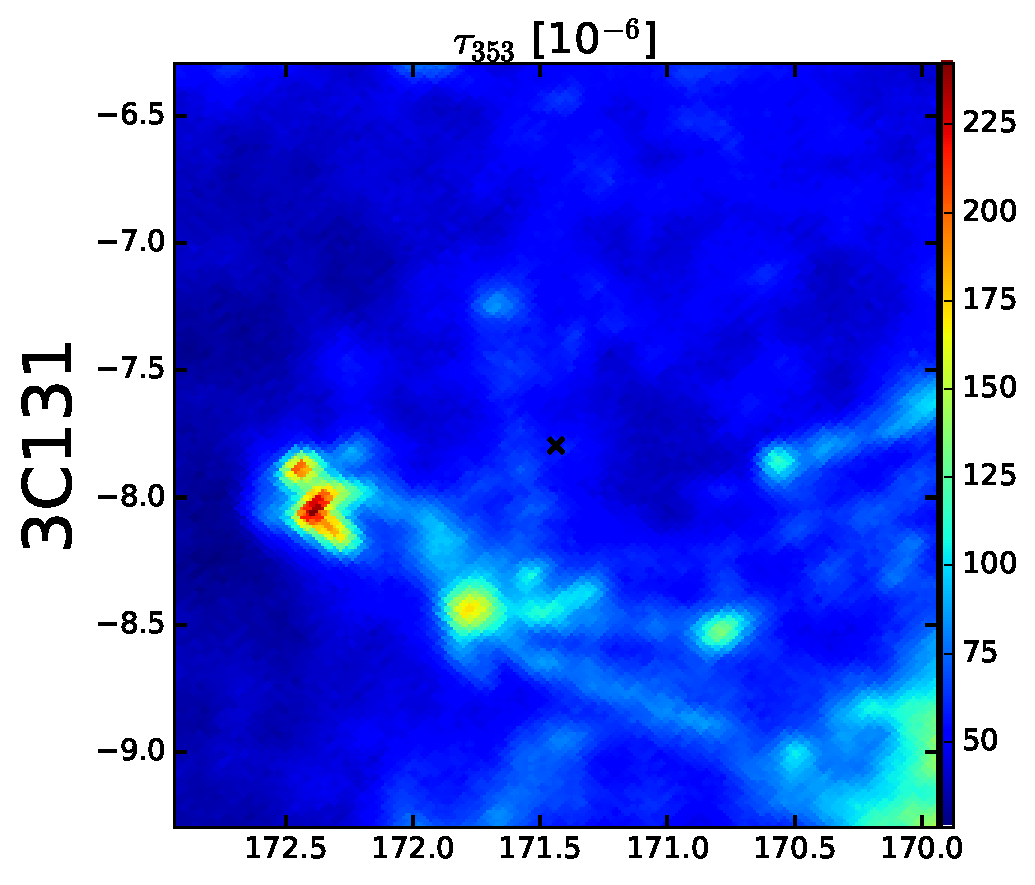
\includegraphics[scale=0.23]{fig/src_eg_apd0_r0c0.eps}
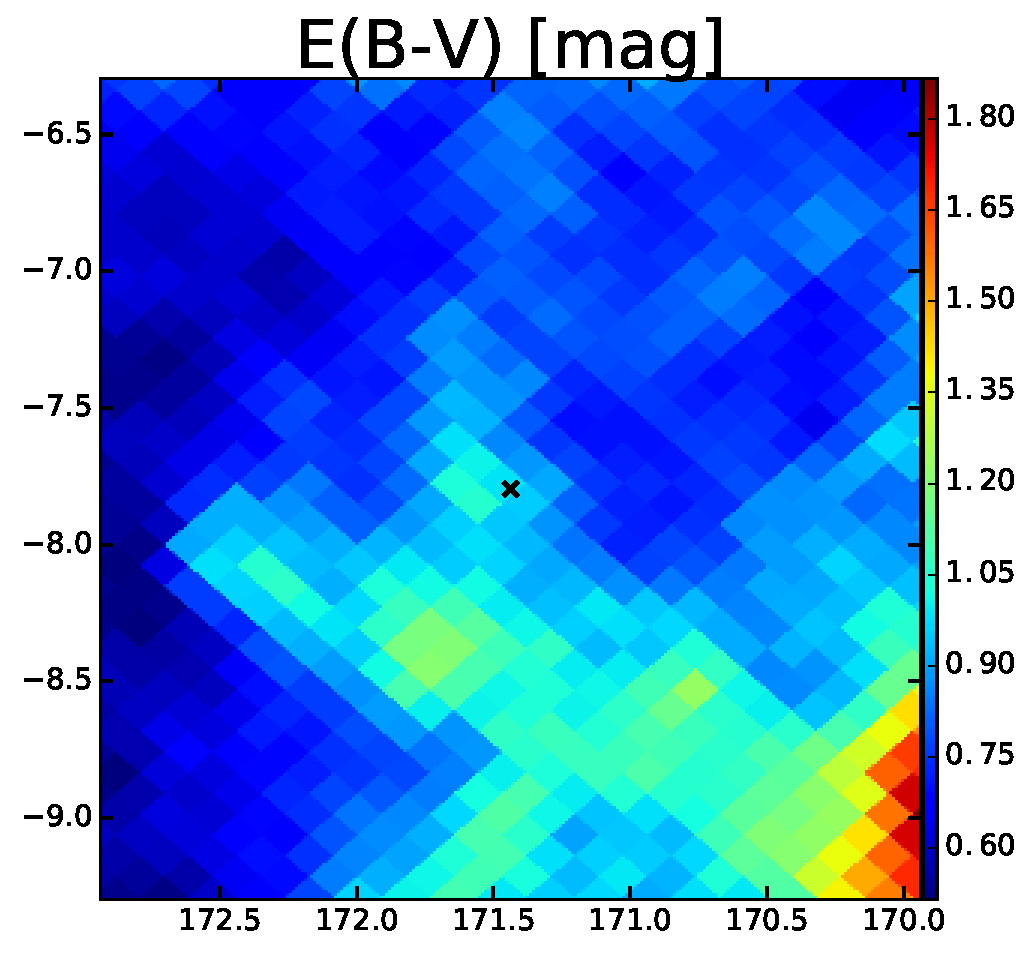
\includegraphics[scale=0.21]{fig/src_eg_apd0_r0c1.eps}
\includegraphics[scale=0.21]{fig/src_eg_apd0_r0c2.eps}
\includegraphics[scale=0.21]{fig/src_eg_apd0_r0c3.eps}
%

\includegraphics[scale=0.23]{fig/src_eg_apd0_r1c0.eps}
\includegraphics[scale=0.21]{fig/src_eg_apd0_r1c1.eps}
\includegraphics[scale=0.21]{fig/src_eg_apd0_r1c2.eps}
\includegraphics[scale=0.21]{fig/src_eg_apd0_r1c3.eps}
%

\includegraphics[scale=0.23]{fig/src_eg_apd0_r2c0.eps}
\includegraphics[scale=0.21]{fig/src_eg_apd0_r2c1.eps}
\includegraphics[scale=0.21]{fig/src_eg_apd0_r2c2.eps}
\includegraphics[scale=0.21]{fig/src_eg_apd0_r2c3.eps}
%
\caption{See Figure \ref{fig:apd0} for details.}
\label{fig:apd3}
\end{figure*}

\begin{figure*}
\centering     
\includegraphics[scale=0.23]{fig/src_eg_apd0_r0c0.eps}
\includegraphics[scale=0.21]{fig/src_eg_apd0_r0c1.eps}
\includegraphics[scale=0.21]{fig/src_eg_apd0_r0c2.eps}
\includegraphics[scale=0.21]{fig/src_eg_apd0_r0c3.eps}
%

\includegraphics[scale=0.23]{fig/src_eg_apd0_r1c0.eps}
\includegraphics[scale=0.21]{fig/src_eg_apd0_r1c1.eps}
\includegraphics[scale=0.21]{fig/src_eg_apd0_r1c2.eps}
\includegraphics[scale=0.21]{fig/src_eg_apd0_r1c3.eps}
%

\includegraphics[scale=0.23]{fig/src_eg_apd0_r2c0.eps}
\includegraphics[scale=0.21]{fig/src_eg_apd0_r2c1.eps}
\includegraphics[scale=0.21]{fig/src_eg_apd0_r2c2.eps}
\includegraphics[scale=0.21]{fig/src_eg_apd0_r2c3.eps}
%
\caption{See Figure \ref{fig:apd0} for details.}
\label{fig:apd4}
\end{figure*}




\begin{sidewaystable}[h!]
\fontsize{7}{6}\selectfont
\centering
\caption{Table of Parameters for OH main lines}
\label{table:OH-parameters}
\renewcommand{\arraystretch}{1.5}
\begin{tabular}{ lllllllclllll  }
 \hline
 \hline
\multirow{2}{*}{$Source$} & \multicolumn{1}{c}{\multirow{2}{*}{$l/b$}} & \multicolumn{6}{c}{OH(1665)} & \multicolumn{5}{c}{OH(1667)}\\
\cline{3-7}
\cline{9-13}
 & & \multicolumn{1}{c}{$\tau$} & \multicolumn{1}{c}{$V_{lsr}$} & \multicolumn{1}{c}{$\Delta V$} & \multicolumn{1}{c}{$T_{ex}$} & \multicolumn{1}{c}{$N(OH)$} & & \multicolumn{1}{c}{$\tau$} & \multicolumn{1}{c}{$V_{lsr}$} & \multicolumn{1}{c}{$\Delta V$} & \multicolumn{1}{c}{$T_{ex}$} & \multicolumn{1}{c}{$N(OH)$} \\
 
(Name) & \multicolumn{1}{c}{$(^{o})$} & \multicolumn{1}{c}{$\ $} & \multicolumn{1}{c}{$(km s^{-1})$} & \multicolumn{1}{c}{$(km s^{-1})$} & \multicolumn{1}{c}{$(K)$} & \multicolumn{1}{c}{$(10^{14}cm^{-2})$} & & \multicolumn{1}{c}{$\ $} & \multicolumn{1}{c}{$(km s^{-1})$} & \multicolumn{1}{c}{$(km s^{-1})$} & \multicolumn{1}{c}{$(K)$} & \multicolumn{1}{c}{$(10^{14}cm^{-2})$} \\ 
\hline


3C105 & 187.6/-33.6 & 0.0156 $\pm$ 0.0003 & 8.14 $\pm$ 0.01 & 0.95 $\pm$ 0.03 & 4.65 $\pm$ 1.86 & 0.29 $\pm$ 0.12 & &  0.0265 $\pm$ 0.0004 & 8.17 $\pm$ 0.01 & 0.94 $\pm$ 0.02 & 3.95 $\pm$ 0.95 & 0.23 $\pm$ 0.06 \\
3C105 & 187.6/-33.6 & 0.0062 $\pm$ 0.0003 & 10.22 $\pm$ 0.02 & 0.93 $\pm$ 0.06 & 8.5 $\pm$ 4.89 & 0.21 $\pm$ 0.12 & &  0.0104 $\pm$ 0.0004 & 10.25 $\pm$ 0.02 & 0.96 $\pm$ 0.04 & 7.66 $\pm$ 3.41 & 0.18 $\pm$ 0.08 \\
3C109 & 181.8/-27.8 & 0.0023 $\pm$ 0.0003 & 9.15 $\pm$ 0.11 & 1.03 $\pm$ 0.26 & 18.28 $\pm$ 27.06 & 0.18 $\pm$ 0.27 & &  0.0036 $\pm$ 0.0004 & 9.24 $\pm$ 0.05 & 0.75 $\pm$ 0.12 & 24.58 $\pm$ 8.7 & 0.16 $\pm$ 0.06 \\
3C109 & 181.8/-27.8 & 0.0036 $\pm$ 0.0003 & 10.45 $\pm$ 0.07 & 0.98 $\pm$ 0.15 & 13.97 $\pm$ 5.41 & 0.21 $\pm$ 0.09 & &  0.0053 $\pm$ 0.0004 & 10.55 $\pm$ 0.04 & 1.02 $\pm$ 0.1 & 13.63 $\pm$ 4.48 & 0.18 $\pm$ 0.06 \\
3C123 & 170.6/-11.7 & 0.0191 $\pm$ 0.0007 & 3.65 $\pm$ 0.06 & 1.19 $\pm$ 0.11 & 10.92 $\pm$ 3.26 & 1.05 $\pm$ 0.33 & &  0.0348 $\pm$ 0.0009 & 3.71 $\pm$ 0.04 & 1.22 $\pm$ 0.07 & 10.92 $\pm$ 2.69 & 1.1 $\pm$ 0.28 \\
3C123 & 170.6/-11.7 & 0.0431 $\pm$ 0.0023 & 4.43 $\pm$ 0.01 & 0.53 $\pm$ 0.03 & 8.06 $\pm$ 0.78 & 0.78 $\pm$ 0.09 & &  0.0919 $\pm$ 0.0029 & 4.46 $\pm$ 0.0 & 0.53 $\pm$ 0.01 & 7.7 $\pm$ 0.65 & 0.89 $\pm$ 0.08 \\
3C123 & 170.6/-11.7 & 0.0337 $\pm$ 0.0008 & 5.37 $\pm$ 0.01 & 0.91 $\pm$ 0.03 & 11.59 $\pm$ 4.3 & 1.53 $\pm$ 0.57 & &  0.0784 $\pm$ 0.0009 & 5.47 $\pm$ 0.01 & 0.92 $\pm$ 0.01 & 8.79 $\pm$ 2.57 & 1.5 $\pm$ 0.44 \\
3C131 & 171.4/-7.8 & 0.0065 $\pm$ 0.0005 & 4.55 $\pm$ 0.02 & 0.56 $\pm$ 0.05 & 12.52 $\pm$ 3.59 & 0.19 $\pm$ 0.06 & &  0.0117 $\pm$ 0.0004 & 4.64 $\pm$ 0.01 & 0.78 $\pm$ 0.04 & 6.96 $\pm$ 1.98 & 0.15 $\pm$ 0.04 \\
3C131 & 171.4/-7.8 & 0.0073 $\pm$ 0.0006 & 6.81 $\pm$ 0.06 & 2.91 $\pm$ 0.23 & 8.94 $\pm$ 4.54 & 0.82 $\pm$ 0.42 & &  0.0089 $\pm$ 0.0005 & 5.84 $\pm$ 0.03 & 0.67 $\pm$ 0.08 & 11.04 $\pm$ 2.07 & 0.16 $\pm$ 0.04 \\
3C131 & 171.4/-7.8 & 0.0166 $\pm$ 0.0007 & 6.59 $\pm$ 0.01 & 0.42 $\pm$ 0.02 & 5.69 $\pm$ 0.85 & 0.17 $\pm$ 0.03 & &  0.0319 $\pm$ 0.0007 & 6.55 $\pm$ 0.01 & 0.45 $\pm$ 0.02 & 5.99 $\pm$ 0.84 & 0.2 $\pm$ 0.03 \\
3C131 & 171.4/-7.8 & 0.0521 $\pm$ 0.0007 & 7.23 $\pm$ 0.0 & 0.55 $\pm$ 0.01 & 5.91 $\pm$ 0.64 & 0.72 $\pm$ 0.08 & &  0.0927 $\pm$ 0.0005 & 7.22 $\pm$ 0.0 & 0.65 $\pm$ 0.01 & 5.98 $\pm$ 0.34 & 0.85 $\pm$ 0.05 \\
3C132 & 178.9/-12.5 & 0.0033 $\pm$ 0.0003 & 7.82 $\pm$ 0.04 & 0.9 $\pm$ 0.1 & 15.55 $\pm$ 6.23 & 0.19 $\pm$ 0.08 & &  0.0056 $\pm$ 0.0003 & 7.79 $\pm$ 0.02 & 0.79 $\pm$ 0.06 & 23.56 $\pm$ 2.17 & 0.25 $\pm$ 0.03 \\
3C133 & 177.7/-9.9 & 0.1008 $\pm$ 0.001 & 7.66 $\pm$ 0.0 & 0.53 $\pm$ 0.0 & 4.47 $\pm$ 0.44 & 1.01 $\pm$ 0.1 & &  0.2132 $\pm$ 0.0014 & 7.68 $\pm$ 0.0 & 0.52 $\pm$ 0.0 & 3.25 $\pm$ 0.27 & 0.85 $\pm$ 0.07 \\
3C133 & 177.7/-9.9 & 0.0149 $\pm$ 0.001 & 7.94 $\pm$ 0.02 & 1.22 $\pm$ 0.04 & 7.08 $\pm$ 3.08 & 0.55 $\pm$ 0.24 & &  0.0333 $\pm$ 0.0013 & 7.96 $\pm$ 0.01 & 1.23 $\pm$ 0.02 & 4.17 $\pm$ 0.99 & 0.4 $\pm$ 0.1 \\
3C154 & 185.6/4.0 & 0.0266 $\pm$ 0.0006 & -2.32 $\pm$ 0.02 & 0.74 $\pm$ 0.03 & 2.69 $\pm$ 1.93 & 0.23 $\pm$ 0.16 & &  0.0429 $\pm$ 0.0006 & -2.34 $\pm$ 0.01 & 0.71 $\pm$ 0.02 & 2.57 $\pm$ 0.75 & 0.19 $\pm$ 0.05 \\
3C154 & 185.6/4.0 & 0.01 $\pm$ 0.0006 & -1.39 $\pm$ 0.04 & 0.83 $\pm$ 0.09 & 5.2 $\pm$ 5.28 & 0.18 $\pm$ 0.19 & &  0.0181 $\pm$ 0.0005 & -1.34 $\pm$ 0.02 & 0.94 $\pm$ 0.05 & 4.46 $\pm$ 1.79 & 0.18 $\pm$ 0.07 \\
3C154 & 185.6/4.0 & 0.0038 $\pm$ 0.0005 & 2.23 $\pm$ 0.07 & 1.14 $\pm$ 0.17 & 5.83 $\pm$ 6.56 & 0.11 $\pm$ 0.12 & &  0.0054 $\pm$ 0.0004 & 2.19 $\pm$ 0.05 & 1.57 $\pm$ 0.13 & 0.54 $\pm$ 8.69 & 0.01 $\pm$ 0.17 \\
3C167 & 207.3/1.2 & 0.0106 $\pm$ 0.0019 & 18.46 $\pm$ 0.12 & 1.49 $\pm$ 0.35 & 4.75 $\pm$ 17.95 & 0.32 $\pm$ 1.22 & &  0.009 $\pm$ 0.0018 & 17.77 $\pm$ 0.15 & 1.76 $\pm$ 0.49 & 4.59 $\pm$ 9.57 & 0.17 $\pm$ 0.36 \\
3C18 & 118.6/-52.7 & 0.0031 $\pm$ 0.0003 & -8.52 $\pm$ 0.11 & 2.64 $\pm$ 0.27 & 10.92 $\pm$ 14.88 & 0.38 $\pm$ 0.52 & &  0.006 $\pm$ 0.0003 & -8.34 $\pm$ 0.05 & 2.61 $\pm$ 0.14 & 9.2 $\pm$ 6.04 & 0.34 $\pm$ 0.23 \\
3C18 & 118.6/-52.7 & 0.0056 $\pm$ 0.0004 & -7.82 $\pm$ 0.02 & 0.67 $\pm$ 0.07 & 6.45 $\pm$ 3.7 & 0.1 $\pm$ 0.06 & &  0.0079 $\pm$ 0.0004 & -7.85 $\pm$ 0.01 & 0.6 $\pm$ 0.04 & 4.83 $\pm$ 1.6 & 0.05 $\pm$ 0.02 \\
3C207 & 213.0/30.1 & 0.015 $\pm$ 0.0002 & 4.55 $\pm$ 0.01 & 0.76 $\pm$ 0.01 & 2.94 $\pm$ 1.55 & 0.14 $\pm$ 0.08 & &  0.0266 $\pm$ 0.0002 & 4.55 $\pm$ 0.0 & 0.77 $\pm$ 0.01 & 2.48 $\pm$ 0.46 & 0.12 $\pm$ 0.02 \\
3C409 & 63.4/-6.1 & 0.0058 $\pm$ 0.0011 & 14.59 $\pm$ 0.27 & 1.68 $\pm$ 0.35 & 11.31 $\pm$ 8.53 & 0.47 $\pm$ 0.38 & &  0.0055 $\pm$ 0.0015 & 14.68 $\pm$ 0.33 & 1.52 $\pm$ 0.4 & 7.83 $\pm$ 11.73 & 0.16 $\pm$ 0.24 \\
3C409 & 63.4/-6.1 & 0.0204 $\pm$ 0.0025 & 15.4 $\pm$ 0.01 & 0.89 $\pm$ 0.05 & 3.18 $\pm$ 2.31 & 0.25 $\pm$ 0.18 & &  0.0275 $\pm$ 0.0032 & 15.42 $\pm$ 0.01 & 0.86 $\pm$ 0.04 & 0.62 $\pm$ 1.0 & 0.03 $\pm$ 0.06 \\
3C410 & 69.2/-3.8 & 0.0044 $\pm$ 0.0006 & 6.32 $\pm$ 0.04 & 1.89 $\pm$ 0.15 & 13.41 $\pm$ 11.22 & 0.47 $\pm$ 0.4 & &  0.0079 $\pm$ 0.0005 & 6.38 $\pm$ 0.02 & 2.32 $\pm$ 0.09 & 6.4 $\pm$ 5.25 & 0.28 $\pm$ 0.23 \\
3C410 & 69.2/-3.8 & 0.0089 $\pm$ 0.0006 & 6.21 $\pm$ 0.01 & 0.65 $\pm$ 0.04 & 8.46 $\pm$ 2.4 & 0.21 $\pm$ 0.06 & &  0.0193 $\pm$ 0.0005 & 6.26 $\pm$ 0.01 & 0.81 $\pm$ 0.02 & 3.81 $\pm$ 1.28 & 0.14 $\pm$ 0.05 \\
3C410 & 69.2/-3.8 & 0.0044 $\pm$ 0.0003 & 10.7 $\pm$ 0.03 & 0.71 $\pm$ 0.07 & 10.06 $\pm$ 5.89 & 0.13 $\pm$ 0.08 & &  0.0085 $\pm$ 0.0002 & 10.71 $\pm$ 0.02 & 0.81 $\pm$ 0.04 & 4.15 $\pm$ 3.09 & 0.07 $\pm$ 0.05 \\
3C410 & 69.2/-3.8 & 0.0054 $\pm$ 0.0002 & 11.67 $\pm$ 0.03 & 0.84 $\pm$ 0.07 & 4.83 $\pm$ 4.66 & 0.09 $\pm$ 0.09 & &  0.0115 $\pm$ 0.0002 & 11.68 $\pm$ 0.02 & 0.82 $\pm$ 0.03 & 2.93 $\pm$ 3.0 & 0.07 $\pm$ 0.07 \\
3C454.3 & 86.1/-38.2 & 0.0023 $\pm$ 0.0001 & -9.67 $\pm$ 0.03 & 1.6 $\pm$ 0.09 & 4.63 $\pm$ 12.36 & 0.07 $\pm$ 0.19 & &  0.0044 $\pm$ 0.0001 & -9.54 $\pm$ 0.01 & 1.25 $\pm$ 0.04 & 8.13 $\pm$ 6.06 & 0.1 $\pm$ 0.08 \\
3C75 & 170.3/-44.9 & 0.0071 $\pm$ 0.0005 & -10.36 $\pm$ 0.04 & 1.3 $\pm$ 0.12 & 3.45 $\pm$ 5.41 & 0.14 $\pm$ 0.21 & &  0.014 $\pm$ 0.0008 & -10.36 $\pm$ 0.03 & 1.22 $\pm$ 0.09 & 3.51 $\pm$ 1.56 & 0.14 $\pm$ 0.06 \\
4C13.67 & 43.5/9.2 & 0.0464 $\pm$ 0.0043 & 4.85 $\pm$ 0.05 & 1.1 $\pm$ 0.12 & 10.43 $\pm$ 2.77 & 2.28 $\pm$ 0.69 & &  0.0567 $\pm$ 0.0057 & 4.89 $\pm$ 0.05 & 1.12 $\pm$ 0.14 & 10.34 $\pm$ 2.13 & 1.55 $\pm$ 0.4 \\
4C22.12 & 188.1/0.0 & 0.0058 $\pm$ 0.001 & -2.84 $\pm$ 0.07 & 0.79 $\pm$ 0.19 & 6.54 $\pm$ 7.03 & 0.13 $\pm$ 0.14 & &  0.0102 $\pm$ 0.0011 & -2.73 $\pm$ 0.04 & 0.78 $\pm$ 0.12 & 6.72 $\pm$ 2.32 & 0.13 $\pm$ 0.05 \\
4C22.12 & 188.1/0.0 & 0.0172 $\pm$ 0.0012 & -1.78 $\pm$ 0.02 & 0.56 $\pm$ 0.05 & 5.07 $\pm$ 2.12 & 0.21 $\pm$ 0.09 & &  0.0354 $\pm$ 0.0013 & -1.78 $\pm$ 0.01 & 0.54 $\pm$ 0.03 & 3.78 $\pm$ 0.74 & 0.17 $\pm$ 0.03 \\
G196.6+0.2 & 196.6/0.2 & 0.0044 $\pm$ 0.0005 & 3.26 $\pm$ 0.11 & 1.94 $\pm$ 0.27 & 10.82 $\pm$ 12.22 & 0.4 $\pm$ 0.46 & &  0.0062 $\pm$ 0.0005 & 3.4 $\pm$ 0.09 & 2.38 $\pm$ 0.22 & 8.85 $\pm$ 8.6 & 0.31 $\pm$ 0.3 \\
G197.0+1.1 & 197.0/1.1 & 0.0126 $\pm$ 0.0005 & 4.83 $\pm$ 0.04 & 1.88 $\pm$ 0.09 & 6.94 $\pm$ 3.82 & 0.7 $\pm$ 0.39 & &  0.0191 $\pm$ 0.001 & 4.73 $\pm$ 0.04 & 1.65 $\pm$ 0.1 & 4.8 $\pm$ 2.17 & 0.36 $\pm$ 0.16 \\
G197.0+1.1 & 197.0/1.1 & 0.0059 $\pm$ 0.0009 & 7.46 $\pm$ 0.05 & 0.65 $\pm$ 0.11 & 0.31 $\pm$ 10.58 & 0.0 $\pm$ 0.17 & &  0.0078 $\pm$ 0.0015 & 7.34 $\pm$ 0.06 & 0.65 $\pm$ 0.14 & 1.61 $\pm$ 5.87 & 0.02 $\pm$ 0.07 \\
G197.0+1.1 & 197.0/1.1 & 0.0049 $\pm$ 0.0005 & 17.01 $\pm$ 0.12 & 2.47 $\pm$ 0.28 & 10.99 $\pm$ 9.9 & 0.57 $\pm$ 0.52 & &  0.0081 $\pm$ 0.0034 & 16.26 $\pm$ 0.17 & 0.91 $\pm$ 0.3 & 6.45 $\pm$ 2.95 & 0.11 $\pm$ 0.08 \\
G197.0+1.1 & 197.0/1.1 & 0.0052 $\pm$ 0.0015 & 17.59 $\pm$ 0.03 & 0.25 $\pm$ 0.08 & 9.87 $\pm$ 1.81 & 0.05 $\pm$ 0.03 & &  0.0127 $\pm$ 0.0013 & 17.38 $\pm$ 0.2 & 1.46 $\pm$ 0.35 & 5.46 $\pm$ 4.35 & 0.24 $\pm$ 0.2 \\
G197.0+1.1 & 197.0/1.1 & 0.0237 $\pm$ 0.001 & 32.01 $\pm$ 0.01 & 0.57 $\pm$ 0.03 & 4.75 $\pm$ 1.92 & 0.27 $\pm$ 0.11 & &  0.043 $\pm$ 0.0017 & 32.01 $\pm$ 0.01 & 0.54 $\pm$ 0.02 & 3.96 $\pm$ 1.04 & 0.22 $\pm$ 0.06 \\
P0428+20 & 176.8/-18.6 & 0.0014 $\pm$ 0.0002 & 3.6 $\pm$ 0.08 & 1.01 $\pm$ 0.19 & 13.48 $\pm$ 7.8 & 0.08 $\pm$ 0.05 & &  0.0029 $\pm$ 0.0003 & 3.54 $\pm$ 0.03 & 0.69 $\pm$ 0.08 & 4.45 $\pm$ 9.98 & 0.02 $\pm$ 0.05 \\
P0428+20 & 176.8/-18.6 & 0.0075 $\pm$ 0.0002 & 10.7 $\pm$ 0.02 & 1.09 $\pm$ 0.04 & 13.49 $\pm$ 3.45 & 0.47 $\pm$ 0.12 & &  0.0136 $\pm$ 0.0002 & 10.7 $\pm$ 0.01 & 1.1 $\pm$ 0.02 & 12.72 $\pm$ 1.62 & 0.45 $\pm$ 0.06 \\
T0526+24 & 181.4/-5.2 & 0.0172 $\pm$ 0.0073 & 7.55 $\pm$ 0.29 & 1.9 $\pm$ 1.13 & 13.7 $\pm$ 15.65 & 1.91 $\pm$ 2.59 & &  0.043 $\pm$ 0.0102 & 7.56 $\pm$ 0.14 & 2.43 $\pm$ 0.75 & 10.19 $\pm$ 7.5 & 2.52 $\pm$ 2.1 \\
T0629+10 & 201.5/0.5 & 0.0043 $\pm$ 0.0022 & 0.16 $\pm$ 0.0 & 0.65 $\pm$ 0.4 & 4.16 $\pm$ 2.97 & 0.05 $\pm$ 0.05 & &  0.0103 $\pm$ 0.0035 & 0.35 $\pm$ 0.0 & 1.18 $\pm$ 0.41 & 3.25 $\pm$ 1.93 & 0.09 $\pm$ 0.07 \\
T0629+10 & 201.5/0.5 & 0.0387 $\pm$ 0.0074 & 3.14 $\pm$ 0.13 & 1.1 $\pm$ 0.0 & 3.85 $\pm$ 0.47 & 0.7 $\pm$ 0.16 & &  0.0577 $\pm$ 0.0113 & 3.07 $\pm$ 0.14 & 1.1 $\pm$ 0.0 & 4.54 $\pm$ 0.55 & 0.68 $\pm$ 0.16 \\
T0629+10 & 201.5/0.5 & 0.0169 $\pm$ 0.0015 & 1.46 $\pm$ 0.07 & 1.39 $\pm$ 0.26 & 2.19 $\pm$ 2.11 & 0.22 $\pm$ 0.22 & &  0.0281 $\pm$ 0.0029 & 1.51 $\pm$ 0.08 & 1.23 $\pm$ 0.25 & 2.9 $\pm$ 0.91 & 0.24 $\pm$ 0.09 \\
T0629+10 & 201.5/0.5 & 0.1607 $\pm$ 0.0104 & 3.6 $\pm$ 0.01 & 0.61 $\pm$ 0.02 & 3.83 $\pm$ 0.35 & 1.59 $\pm$ 0.19 & &  0.2536 $\pm$ 0.0154 & 3.6 $\pm$ 0.01 & 0.65 $\pm$ 0.03 & 4.72 $\pm$ 0.64 & 1.84 $\pm$ 0.29 \\
T0629+10 & 201.5/0.5 & 0.0811 $\pm$ 0.002 & 4.62 $\pm$ 0.01 & 0.76 $\pm$ 0.03 & 6.43 $\pm$ 0.97 & 1.68 $\pm$ 0.27 & &  0.1553 $\pm$ 0.0037 & 4.61 $\pm$ 0.01 & 0.67 $\pm$ 0.03 & 6.62 $\pm$ 1.01 & 1.63 $\pm$ 0.26 \\
T0629+10 & 201.5/0.5 & 0.0747 $\pm$ 0.0018 & 6.09 $\pm$ 0.02 & 1.06 $\pm$ 0.05 & 5.44 $\pm$ 1.58 & 1.84 $\pm$ 0.54 & &  0.1165 $\pm$ 0.003 & 6.06 $\pm$ 0.02 & 1.17 $\pm$ 0.07 & 6.52 $\pm$ 1.67 & 2.1 $\pm$ 0.55 \\
T0629+10 & 201.5/0.5 & 0.0367 $\pm$ 0.0031 & 7.0 $\pm$ 0.02 & 0.49 $\pm$ 0.06 & 4.36 $\pm$ 0.68 & 0.33 $\pm$ 0.07 & &  0.0631 $\pm$ 0.0056 & 7.0 $\pm$ 0.02 & 0.5 $\pm$ 0.06 & 4.2 $\pm$ 0.3 & 0.31 $\pm$ 0.05 \\
T0629+10 & 201.5/0.5 & 0.0174 $\pm$ 0.0018 & 7.9 $\pm$ 0.05 & 0.83 $\pm$ 0.13 & 3.44 $\pm$ 1.67 & 0.21 $\pm$ 0.11 & &  0.0307 $\pm$ 0.003 & 7.91 $\pm$ 0.05 & 0.82 $\pm$ 0.13 & 3.65 $\pm$ 1.21 & 0.22 $\pm$ 0.08 \\



\hline
\end{tabular}
\end{sidewaystable}


\end{document}

%%% THE END %%%



 - ..}